% Options for packages loaded elsewhere
% Options for packages loaded elsewhere
\PassOptionsToPackage{unicode}{hyperref}
\PassOptionsToPackage{hyphens}{url}
\PassOptionsToPackage{dvipsnames,svgnames,x11names}{xcolor}
%
\documentclass[
  letterpaper,
  DIV=11,
  numbers=noendperiod]{scrreprt}
\usepackage{xcolor}
\usepackage{amsmath,amssymb}
\setcounter{secnumdepth}{5}
\usepackage{iftex}
\ifPDFTeX
  \usepackage[T1]{fontenc}
  \usepackage[utf8]{inputenc}
  \usepackage{textcomp} % provide euro and other symbols
\else % if luatex or xetex
  \usepackage{unicode-math} % this also loads fontspec
  \defaultfontfeatures{Scale=MatchLowercase}
  \defaultfontfeatures[\rmfamily]{Ligatures=TeX,Scale=1}
\fi
\usepackage{lmodern}
\ifPDFTeX\else
  % xetex/luatex font selection
\fi
% Use upquote if available, for straight quotes in verbatim environments
\IfFileExists{upquote.sty}{\usepackage{upquote}}{}
\IfFileExists{microtype.sty}{% use microtype if available
  \usepackage[]{microtype}
  \UseMicrotypeSet[protrusion]{basicmath} % disable protrusion for tt fonts
}{}
\makeatletter
\@ifundefined{KOMAClassName}{% if non-KOMA class
  \IfFileExists{parskip.sty}{%
    \usepackage{parskip}
  }{% else
    \setlength{\parindent}{0pt}
    \setlength{\parskip}{6pt plus 2pt minus 1pt}}
}{% if KOMA class
  \KOMAoptions{parskip=half}}
\makeatother
% Make \paragraph and \subparagraph free-standing
\makeatletter
\ifx\paragraph\undefined\else
  \let\oldparagraph\paragraph
  \renewcommand{\paragraph}{
    \@ifstar
      \xxxParagraphStar
      \xxxParagraphNoStar
  }
  \newcommand{\xxxParagraphStar}[1]{\oldparagraph*{#1}\mbox{}}
  \newcommand{\xxxParagraphNoStar}[1]{\oldparagraph{#1}\mbox{}}
\fi
\ifx\subparagraph\undefined\else
  \let\oldsubparagraph\subparagraph
  \renewcommand{\subparagraph}{
    \@ifstar
      \xxxSubParagraphStar
      \xxxSubParagraphNoStar
  }
  \newcommand{\xxxSubParagraphStar}[1]{\oldsubparagraph*{#1}\mbox{}}
  \newcommand{\xxxSubParagraphNoStar}[1]{\oldsubparagraph{#1}\mbox{}}
\fi
\makeatother

\usepackage{color}
\usepackage{fancyvrb}
\newcommand{\VerbBar}{|}
\newcommand{\VERB}{\Verb[commandchars=\\\{\}]}
\DefineVerbatimEnvironment{Highlighting}{Verbatim}{commandchars=\\\{\}}
% Add ',fontsize=\small' for more characters per line
\usepackage{framed}
\definecolor{shadecolor}{RGB}{241,243,245}
\newenvironment{Shaded}{\begin{snugshade}}{\end{snugshade}}
\newcommand{\AlertTok}[1]{\textcolor[rgb]{0.68,0.00,0.00}{#1}}
\newcommand{\AnnotationTok}[1]{\textcolor[rgb]{0.37,0.37,0.37}{#1}}
\newcommand{\AttributeTok}[1]{\textcolor[rgb]{0.40,0.45,0.13}{#1}}
\newcommand{\BaseNTok}[1]{\textcolor[rgb]{0.68,0.00,0.00}{#1}}
\newcommand{\BuiltInTok}[1]{\textcolor[rgb]{0.00,0.23,0.31}{#1}}
\newcommand{\CharTok}[1]{\textcolor[rgb]{0.13,0.47,0.30}{#1}}
\newcommand{\CommentTok}[1]{\textcolor[rgb]{0.37,0.37,0.37}{#1}}
\newcommand{\CommentVarTok}[1]{\textcolor[rgb]{0.37,0.37,0.37}{\textit{#1}}}
\newcommand{\ConstantTok}[1]{\textcolor[rgb]{0.56,0.35,0.01}{#1}}
\newcommand{\ControlFlowTok}[1]{\textcolor[rgb]{0.00,0.23,0.31}{\textbf{#1}}}
\newcommand{\DataTypeTok}[1]{\textcolor[rgb]{0.68,0.00,0.00}{#1}}
\newcommand{\DecValTok}[1]{\textcolor[rgb]{0.68,0.00,0.00}{#1}}
\newcommand{\DocumentationTok}[1]{\textcolor[rgb]{0.37,0.37,0.37}{\textit{#1}}}
\newcommand{\ErrorTok}[1]{\textcolor[rgb]{0.68,0.00,0.00}{#1}}
\newcommand{\ExtensionTok}[1]{\textcolor[rgb]{0.00,0.23,0.31}{#1}}
\newcommand{\FloatTok}[1]{\textcolor[rgb]{0.68,0.00,0.00}{#1}}
\newcommand{\FunctionTok}[1]{\textcolor[rgb]{0.28,0.35,0.67}{#1}}
\newcommand{\ImportTok}[1]{\textcolor[rgb]{0.00,0.46,0.62}{#1}}
\newcommand{\InformationTok}[1]{\textcolor[rgb]{0.37,0.37,0.37}{#1}}
\newcommand{\KeywordTok}[1]{\textcolor[rgb]{0.00,0.23,0.31}{\textbf{#1}}}
\newcommand{\NormalTok}[1]{\textcolor[rgb]{0.00,0.23,0.31}{#1}}
\newcommand{\OperatorTok}[1]{\textcolor[rgb]{0.37,0.37,0.37}{#1}}
\newcommand{\OtherTok}[1]{\textcolor[rgb]{0.00,0.23,0.31}{#1}}
\newcommand{\PreprocessorTok}[1]{\textcolor[rgb]{0.68,0.00,0.00}{#1}}
\newcommand{\RegionMarkerTok}[1]{\textcolor[rgb]{0.00,0.23,0.31}{#1}}
\newcommand{\SpecialCharTok}[1]{\textcolor[rgb]{0.37,0.37,0.37}{#1}}
\newcommand{\SpecialStringTok}[1]{\textcolor[rgb]{0.13,0.47,0.30}{#1}}
\newcommand{\StringTok}[1]{\textcolor[rgb]{0.13,0.47,0.30}{#1}}
\newcommand{\VariableTok}[1]{\textcolor[rgb]{0.07,0.07,0.07}{#1}}
\newcommand{\VerbatimStringTok}[1]{\textcolor[rgb]{0.13,0.47,0.30}{#1}}
\newcommand{\WarningTok}[1]{\textcolor[rgb]{0.37,0.37,0.37}{\textit{#1}}}

\usepackage{longtable,booktabs,array}
\usepackage{calc} % for calculating minipage widths
% Correct order of tables after \paragraph or \subparagraph
\usepackage{etoolbox}
\makeatletter
\patchcmd\longtable{\par}{\if@noskipsec\mbox{}\fi\par}{}{}
\makeatother
% Allow footnotes in longtable head/foot
\IfFileExists{footnotehyper.sty}{\usepackage{footnotehyper}}{\usepackage{footnote}}
\makesavenoteenv{longtable}
\usepackage{graphicx}
\makeatletter
\newsavebox\pandoc@box
\newcommand*\pandocbounded[1]{% scales image to fit in text height/width
  \sbox\pandoc@box{#1}%
  \Gscale@div\@tempa{\textheight}{\dimexpr\ht\pandoc@box+\dp\pandoc@box\relax}%
  \Gscale@div\@tempb{\linewidth}{\wd\pandoc@box}%
  \ifdim\@tempb\p@<\@tempa\p@\let\@tempa\@tempb\fi% select the smaller of both
  \ifdim\@tempa\p@<\p@\scalebox{\@tempa}{\usebox\pandoc@box}%
  \else\usebox{\pandoc@box}%
  \fi%
}
% Set default figure placement to htbp
\def\fps@figure{htbp}
\makeatother





\setlength{\emergencystretch}{3em} % prevent overfull lines

\providecommand{\tightlist}{%
  \setlength{\itemsep}{0pt}\setlength{\parskip}{0pt}}



 


\KOMAoption{captions}{tableheading}
\makeatletter
\@ifpackageloaded{tcolorbox}{}{\usepackage[skins,breakable]{tcolorbox}}
\@ifpackageloaded{fontawesome5}{}{\usepackage{fontawesome5}}
\definecolor{quarto-callout-color}{HTML}{909090}
\definecolor{quarto-callout-note-color}{HTML}{0758E5}
\definecolor{quarto-callout-important-color}{HTML}{CC1914}
\definecolor{quarto-callout-warning-color}{HTML}{EB9113}
\definecolor{quarto-callout-tip-color}{HTML}{00A047}
\definecolor{quarto-callout-caution-color}{HTML}{FC5300}
\definecolor{quarto-callout-color-frame}{HTML}{acacac}
\definecolor{quarto-callout-note-color-frame}{HTML}{4582ec}
\definecolor{quarto-callout-important-color-frame}{HTML}{d9534f}
\definecolor{quarto-callout-warning-color-frame}{HTML}{f0ad4e}
\definecolor{quarto-callout-tip-color-frame}{HTML}{02b875}
\definecolor{quarto-callout-caution-color-frame}{HTML}{fd7e14}
\makeatother
\makeatletter
\@ifpackageloaded{bookmark}{}{\usepackage{bookmark}}
\makeatother
\makeatletter
\@ifpackageloaded{caption}{}{\usepackage{caption}}
\AtBeginDocument{%
\ifdefined\contentsname
  \renewcommand*\contentsname{Table of contents}
\else
  \newcommand\contentsname{Table of contents}
\fi
\ifdefined\listfigurename
  \renewcommand*\listfigurename{List of Figures}
\else
  \newcommand\listfigurename{List of Figures}
\fi
\ifdefined\listtablename
  \renewcommand*\listtablename{List of Tables}
\else
  \newcommand\listtablename{List of Tables}
\fi
\ifdefined\figurename
  \renewcommand*\figurename{Figure}
\else
  \newcommand\figurename{Figure}
\fi
\ifdefined\tablename
  \renewcommand*\tablename{Table}
\else
  \newcommand\tablename{Table}
\fi
}
\@ifpackageloaded{float}{}{\usepackage{float}}
\floatstyle{ruled}
\@ifundefined{c@chapter}{\newfloat{codelisting}{h}{lop}}{\newfloat{codelisting}{h}{lop}[chapter]}
\floatname{codelisting}{Listing}
\newcommand*\listoflistings{\listof{codelisting}{List of Listings}}
\makeatother
\makeatletter
\makeatother
\makeatletter
\@ifpackageloaded{caption}{}{\usepackage{caption}}
\@ifpackageloaded{subcaption}{}{\usepackage{subcaption}}
\makeatother
\usepackage{bookmark}
\IfFileExists{xurl.sty}{\usepackage{xurl}}{} % add URL line breaks if available
\urlstyle{same}
\hypersetup{
  pdftitle={Information Visualization and the Humanities: Course Book},
  pdfauthor={Yann Ryan},
  colorlinks=true,
  linkcolor={blue},
  filecolor={Maroon},
  citecolor={Blue},
  urlcolor={Blue},
  pdfcreator={LaTeX via pandoc}}


\title{Information Visualization and the Humanities: Course Book}
\author{Yann Ryan}
\date{2024-09-01}
\begin{document}
\maketitle

\renewcommand*\contentsname{Table of contents}
{
\hypersetup{linkcolor=}
\setcounter{tocdepth}{2}
\tableofcontents
}

\bookmarksetup{startatroot}

\chapter*{Course Overview}\label{course-overview}
\addcontentsline{toc}{chapter}{Course Overview}

\markboth{Course Overview}{Course Overview}

Welcome! You're probably here because you are taking the course
\emph{Information Visualization and the Humanities,} taking place in
Semester 1, 2025-2026, at Leiden University. It's part of the minor in
Digital Humanities. The course instructor is Dr.~Yann Ryan.

This e-book will serve as the course website. The menu on the left side
lists the chapters, one for each week of the course. More will appear as
the course progresses. The menu on the right contains the table of
contents for this particular chapter, so you can skip to different
sections. There's a search function just below the title on the left,
which students have found very useful when they want to find some code
we've discussed and use it later on in an assignment.

You'll also need to familiarise yourself with the course
\href{https://brightspace.universiteitleiden.nl/d2l/home/402636}{Brightspace
area}, where I'll put further information and you'll submit assignments.

\section*{What do we mean by `information
visualisation'?}\label{what-do-we-mean-by-information-visualisation}
\addcontentsline{toc}{section}{What do we mean by `information
visualisation'?}

\markright{What do we mean by `information visualisation'?}

Information visualization (or data visualization, which I'll use
interchangeablely) could be defined as \textbf{\emph{the graphical
representation of information and data}}.

Data visualization is often used to convey or communicate messages about
complex or large-scale data. It has been around in its present
form---charts, graphs and so forth---since at least the eighteenth
century. One form of data visualisation---maps---have been around for
even longer. Today, we come across data visualizations in our daily
lives: in everything from scientific articles to news media, and in
advertisements.

In the humanities, the data we use might be, for example, historical
statistics or networks, or the text (or data derived from it) found in
literary works. It might be something totally different such as audio,
images, or spatial data.

\section*{Course Aims and Objectives}\label{course-aims-and-objectives}
\addcontentsline{toc}{section}{Course Aims and Objectives}

\markright{Course Aims and Objectives}

\begin{itemize}
\item
  At the end of this course, you will:

  \begin{itemize}
  \item
    Be able to construct data visualisations from scratch using the
    coding language R.
  \item
    Use online publication formats such as Markdown to make
    professional-standard visual essays containing code, visualisations,
    and explanatory text.
  \item
    Understand how a FAIR (Findable, Accessible, Interoperable, and
    Reusable) approach to data is important for your work and that of
    others.
  \item
    Be able to critically reflect on a range of visualizations, with a
    specific focus on network and spatial data.
  \item
    Know where to find some of the inspiring visualizations, thinkers,
    and designers in this field.
  \item
    Be able to discuss your views on information visualization with
    peers as well as give and receive feedback.
  \end{itemize}
\end{itemize}

In terms of concrete skills, by the end of this course, you should be
able to use humanities-focused data to make informative,
highly-customised visualisations such as this:

\begin{Shaded}
\begin{Highlighting}[]
\FunctionTok{library}\NormalTok{(tidyverse)}
\FunctionTok{library}\NormalTok{(ggthemes)}

\FunctionTok{options}\NormalTok{(}\AttributeTok{scipen =} \DecValTok{999999}\NormalTok{)}

\NormalTok{df }\OtherTok{=}\NormalTok{ data.table}\SpecialCharTok{::}\FunctionTok{fread}\NormalTok{(}\StringTok{\textquotesingle{}box\_office.csv\textquotesingle{}}\NormalTok{)}

\NormalTok{df }\OtherTok{=}\NormalTok{ df }\SpecialCharTok{\%\textgreater{}\%} 
  \FunctionTok{mutate}\NormalTok{(}\AttributeTok{billions =}\NormalTok{total\_inflation\_adjusted\_box\_office}\SpecialCharTok{/}\DecValTok{1000000000}\NormalTok{ )}

\FunctionTok{ggplot}\NormalTok{() }\SpecialCharTok{+} 
  \FunctionTok{geom\_point}\NormalTok{(}\AttributeTok{data =}\NormalTok{ df, }\FunctionTok{aes}\NormalTok{(year, }\FunctionTok{as.numeric}\NormalTok{(billions)), }\AttributeTok{size=} \DecValTok{1}\NormalTok{, }\AttributeTok{alpha =}\NormalTok{ .}\DecValTok{5}\NormalTok{) }\SpecialCharTok{+}
  \FunctionTok{geom\_smooth}\NormalTok{(}\AttributeTok{data =}\NormalTok{ df, }\FunctionTok{aes}\NormalTok{(year, }\FunctionTok{as.numeric}\NormalTok{(billions)), }\AttributeTok{method =} \StringTok{"lm"}\NormalTok{,}
              \AttributeTok{formula =}\NormalTok{ y }\SpecialCharTok{\textasciitilde{}} \FunctionTok{poly}\NormalTok{(x, }\DecValTok{23}\NormalTok{), }\AttributeTok{se =} \ConstantTok{FALSE}\NormalTok{, }\AttributeTok{color =} \StringTok{\textquotesingle{}black\textquotesingle{}}\NormalTok{, }\AttributeTok{alpha =}\NormalTok{ .}\DecValTok{75}\NormalTok{) }\SpecialCharTok{+} 
  \FunctionTok{scale\_y\_continuous}\NormalTok{(}\AttributeTok{limits =} \FunctionTok{c}\NormalTok{(}\DecValTok{0}\NormalTok{, }\DecValTok{15}\NormalTok{)) }\SpecialCharTok{+} 
  \FunctionTok{labs}\NormalTok{(}\AttributeTok{title =} \StringTok{\textquotesingle{}Domestic Yearly Box Office, 1995 to 2023\textquotesingle{}}\NormalTok{, }
       \AttributeTok{subtitle =} \StringTok{"In billion US dollars, adjusted for inflation"}\NormalTok{, }
       \AttributeTok{x =} \ConstantTok{NULL}\NormalTok{, }
       \AttributeTok{y =} \StringTok{"Box office in billions US (inflation adjusted)"}\NormalTok{)  }\SpecialCharTok{+}
  \FunctionTok{geom\_vline}\NormalTok{(}\AttributeTok{xintercept=}\DecValTok{2020}\NormalTok{, }\AttributeTok{color =} \StringTok{\textquotesingle{}red\textquotesingle{}}\NormalTok{, }\AttributeTok{alpha =}\NormalTok{ .}\DecValTok{6}\NormalTok{, }\AttributeTok{size =} \DecValTok{2}\NormalTok{) }\SpecialCharTok{+}
  \FunctionTok{annotate}\NormalTok{(}\StringTok{"text"}\NormalTok{, }\AttributeTok{x=}\DecValTok{2019}\NormalTok{, }\AttributeTok{y=}\DecValTok{5}\NormalTok{, }\AttributeTok{label=}\StringTok{"First Pandemic Year"}\NormalTok{, }\AttributeTok{angle=}\DecValTok{90}\NormalTok{) }\SpecialCharTok{+} 
  \FunctionTok{theme\_economist}\NormalTok{()}
\end{Highlighting}
\end{Shaded}

\pandocbounded{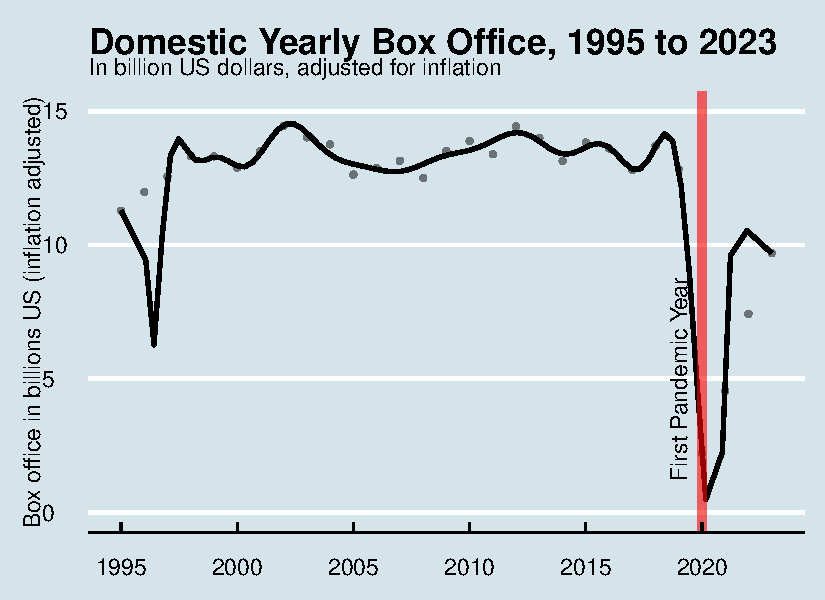
\includegraphics[keepaspectratio]{index_files/figure-pdf/unnamed-chunk-1-1.pdf}}

or this:

\begin{Shaded}
\begin{Highlighting}[]
\FunctionTok{library}\NormalTok{(ggrepel)}

\NormalTok{df2 }\OtherTok{=}\NormalTok{ data.table}\SpecialCharTok{::}\FunctionTok{fread}\NormalTok{(}\StringTok{"top\_movie.csv"}\NormalTok{)}

\NormalTok{df2 }\OtherTok{=}\NormalTok{ df2 }\SpecialCharTok{\%\textgreater{}\%}
  \FunctionTok{mutate}\NormalTok{(}\AttributeTok{billions =}\NormalTok{total\_in\_2022\_dollars}\SpecialCharTok{/}\DecValTok{1000}\NormalTok{)}

\NormalTok{top\_data }\OtherTok{=}\NormalTok{ df2 }\SpecialCharTok{\%\textgreater{}\%} 
  \FunctionTok{slice\_max}\NormalTok{(}\AttributeTok{order\_by =}\NormalTok{ total\_in\_2022\_dollars, }\AttributeTok{n =} \DecValTok{5}\NormalTok{)}

\NormalTok{   p }\OtherTok{=}  \FunctionTok{ggplot}\NormalTok{() }\SpecialCharTok{+} 
      \FunctionTok{geom\_point}\NormalTok{(}\AttributeTok{data =}\NormalTok{ df2,(}\FunctionTok{aes}\NormalTok{(}\AttributeTok{x =}\NormalTok{ year, }
                                 \AttributeTok{y =}\NormalTok{ billions, }
                                 \AttributeTok{size =}\NormalTok{ billions, }
                                 \AttributeTok{fill =}\NormalTok{ distributor)), }
                 \AttributeTok{pch =} \DecValTok{21}\NormalTok{, }\AttributeTok{color =} \StringTok{\textquotesingle{}black\textquotesingle{}}\NormalTok{, }\AttributeTok{alpha =}\NormalTok{ .}\DecValTok{6}\NormalTok{, }\AttributeTok{stroke=}\NormalTok{ .}\DecValTok{5}\NormalTok{) }\SpecialCharTok{+} 
      \FunctionTok{geom\_label\_repel}\NormalTok{(}\AttributeTok{data =}\NormalTok{ top\_data, }\FunctionTok{aes}\NormalTok{(}\AttributeTok{x =}\NormalTok{ year, }
                                            \AttributeTok{y =}\NormalTok{ billions, }
                                            \AttributeTok{label =}\NormalTok{ movie, }
                                            \AttributeTok{fill =}\NormalTok{ distributor), }
                       \AttributeTok{alpha =}\NormalTok{ .}\DecValTok{6}\NormalTok{,}\AttributeTok{show.legend=}\ConstantTok{FALSE}\NormalTok{) }\SpecialCharTok{+} 
      \FunctionTok{scale\_size\_area}\NormalTok{(}\AttributeTok{max\_size =} \DecValTok{6}\NormalTok{) }\SpecialCharTok{+} 
      \FunctionTok{labs}\NormalTok{(}\AttributeTok{title =} \StringTok{"The Rise and Rise of Disney"}\NormalTok{, }
           \AttributeTok{subtitle =} \StringTok{"Nearly 1/3 of the highest{-}grossing movies (in the US) of the last 30 years}\SpecialCharTok{\textbackslash{}n}\StringTok{have been made by the Disney Company"}\NormalTok{) }\SpecialCharTok{+} 
      \FunctionTok{theme\_fivethirtyeight}\NormalTok{() }\SpecialCharTok{+} 
      \FunctionTok{labs}\NormalTok{(}\AttributeTok{y =} \StringTok{"Box office in billions US (inflation adjusted)"}\NormalTok{, }
           \AttributeTok{size =} \StringTok{"Takings (Billions): "}\NormalTok{, }\AttributeTok{fill =} \StringTok{\textquotesingle{}Distributor: \textquotesingle{}}\NormalTok{) }\SpecialCharTok{+} 
      \FunctionTok{theme}\NormalTok{(}\AttributeTok{legend.position =} \StringTok{\textquotesingle{}bottom\textquotesingle{}}\NormalTok{, }
            \AttributeTok{legend.box=}\StringTok{"vertical"}\NormalTok{, }
            \AttributeTok{legend.margin=}\FunctionTok{margin}\NormalTok{())}

                
\NormalTok{p}
\end{Highlighting}
\end{Shaded}

\pandocbounded{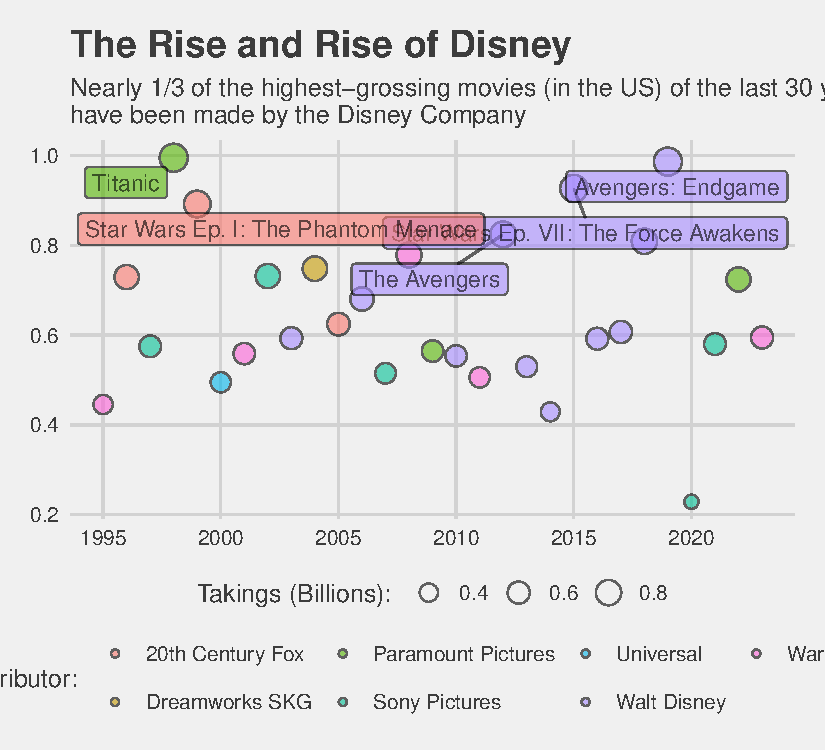
\includegraphics[keepaspectratio]{index_files/figure-pdf/unnamed-chunk-2-1.pdf}}

Perhaps most importantly, you will have total control over every aspect
of the visualisation, from the colours, to the titles, labels, and
scales. Use the `show the code' button above the visualisation to see
the code it was made from.

Your final and most important piece of work will be a \emph{Markdown
report:} a publishable document containing code, text, and data
visualisations. This report will show off all the skills you have
learned during the course.

\subsection*{Information
Visualisation\ldots{}}\label{information-visualisation}
\addcontentsline{toc}{subsection}{Information Visualisation\ldots{}}

Most importantly, you'll learn the basic principles of information
visualization, and put them into practice using a platform called R
(more on that below). R is widely used by, for example, data journalists
at the BBC, and in publications like \emph{The Economist} and the
\emph{Financial Times.}

Using a language like R or python instead of Excel or a simple
application for visualising data has many advantages. For one, it's much
easier to work with large datasets. You want to analyse huge datasets of
movies like \href{https://datasets.imdbws.com/}{these ones}, with 11
millions rows of data? It'll take a split second in R. A second
advantage is that everything you make can be reproducible, meaning your
visualisations and analyses can be scientifically checked and verified.

The visualisations above were made with a few lines of the R language.
If you click the `Show the code' button above them, you'll see the code
I used to create them. It might look a little complicated now, but if
you follow the course, you should be able to make similar (and hopefully
much nicer) ones by the end of the twelve weeks.

In your final project, you'll combine text, data and visual outputs to
make a \emph{report} on a topic you're interested in. You'll make a
document like this. For this course, it's more than enough to stick to
the basic charts like the above. But if you're interested, you can
explore fancier things such as interactive maps and charts, 3D-rendered
visualisations, and more.

\subsection*{\ldots and the Humanities}\label{and-the-humanities}
\addcontentsline{toc}{subsection}{\ldots and the Humanities}

This is not to say the course will be an exhaustive `how to' for
scientific data visualisations. One of your superpowers as a humanities
student is that you learn to to move beyond the surface level and
consider the subtexts, biases, and so forth in cultural objects. In this
course, we'll put those skills to good use, and you'll use your own
expertise and interests to tell compelling and truthful stories about
humanities subjects, using data.

Just as importantly, you'll learn how to critique data visualisations
and design. As a group we'll ask: what makes them good or bad,
scientific or unethical? Can we trust the intentions behind commercial
or political data visualisations? Can we spot when they are being
misleading, and describe exactly \emph{how}? What are the negative and
positive connotations around certain graphical representations, and why
do we use them? How can we make better, more ethical data
visualisations? How can we make visualisations which properly consider
those with accessibility needs?

\section*{Doing not reading.. mostly}\label{doing-not-reading..-mostly}
\addcontentsline{toc}{section}{Doing not reading.. mostly}

\markright{Doing not reading.. mostly}

This will be a `doing' course: you'll spend most of your self-study time
completing at-home exercises and assignments. There will be two
compulsory readings to get a background on some of the wider themes of
the course, which we will discuss in class. The two pieces we'll read
are:

\begin{itemize}
\item
  D'Ignazio, C., \& Klein, L. (2020). 2. Collect, Analyze, Imagine,
  Teach. In Data Feminism. Retrieved from
  https://data-feminism.mitpress.mit.edu/pub/ei7cogfn
\item
  D'Ignazio, C., \& Klein, L. (2020). 3. On Rational, Scientific,
  Objective Viewpoints from Mythical, Imaginary, Impossible Standpoints.
  In Data Feminism. Retrieved from
  https://data-feminism.mitpress.mit.edu/pub/5evfe9yd
\end{itemize}

There will also be some weekly recommended reading if you would like to
dig deeper into topics on your own time. You can find it near the end of
this page.

\section*{Schedule}\label{schedule}
\addcontentsline{toc}{section}{Schedule}

\markright{Schedule}

Below is the course schedule. In the first couple of weeks, you'll learn
how to do the very basics using the coding language R. This will be
followed by three weeks focusing on data analysis, then two blocks of
three: first, data visualisation, and second, digital mapping. We'll
wrap things up with a week on creating polished, publishable data
visualisations, and how to make your charts and maps interactive.

\begin{longtable}[]{@{}
  >{\raggedright\arraybackslash}p{(\linewidth - 8\tabcolsep) * \real{0.0400}}
  >{\raggedright\arraybackslash}p{(\linewidth - 8\tabcolsep) * \real{0.1100}}
  >{\raggedright\arraybackslash}p{(\linewidth - 8\tabcolsep) * \real{0.2800}}
  >{\raggedright\arraybackslash}p{(\linewidth - 8\tabcolsep) * \real{0.2800}}
  >{\raggedright\arraybackslash}p{(\linewidth - 8\tabcolsep) * \real{0.2800}}@{}}
\caption{Course Schedule}\tabularnewline
\toprule\noalign{}
\endfirsthead
\endhead
\bottomrule\noalign{}
\endlastfoot
\textbf{Week} & \textbf{Date} & \textbf{Topic} & \textbf{Topic} &
\textbf{Assignment} \\
1 & 2025-09-08 & Introductions & Tour of the course book & \\
2 & 2025-09-15 & Introduction to R & How to use R and Posit cloud & \\
3 & 2025-09-22 & Data analysis 1 & Working with dataframes. Selecting
and subsetting data. & Discussion of reading 1. \\
4 & 2025-09-29 & Data analysis 2 & Filtering and changing data & \\
5 & 2025-10-06 & Data analysis 3 & Summarising and grouping data & \\
6 & 2025-10-13 & Data visualisation 1 & Getting started with R and
ggplot2. & \\
7 & 2025-10-20 & Data visualisation 2 & Scales and legends & \\
8 & 2025-11-03 & Data visualisation 3 & Annotations and themes & \\
9 & 2025-11-10 & Data visualisation 4 & Ethics, reproducibility, and
accessibility & Assignment 1 (create a datavis) due. Discussion of
reading 2. \\
10 & 2025-11-17 & Digital mapping 1 & Working with R as a GIS. Creating
base maps. & \\
11 & 2025-11-24 & Digital mapping 2 & Importing shapefiles and mapping
external data & \\
12 & 2025-12-01 & Digital mapping 3 & The tmap package & \\
13 & 2025-12-08 & Publication & R Markdown and Interactivity &
Assignment 2 (create a map visualisation) due. \\
& 2026-14-01 & & & Final project due \\
\end{longtable}

\section*{Data Visualisation}\label{data-visualisation}
\addcontentsline{toc}{section}{Data Visualisation}

\markright{Data Visualisation}

In practice, creating data visualisations involves mapping numerical
data of some sort to graphical representations - often called
geometries. A geometry might be the length of a line, the x and y
position on a graph, or the temperature of a colour on a map. A good
data visualisation will use this mapping to tell a story about the data,
while representing it faithfully.

\subsection*{What will I actually do on this
course?}\label{what-will-i-actually-do-on-this-course}
\addcontentsline{toc}{subsection}{What will I actually do on this
course?}

You'll put these skills into practice using a tool called R. R is a
coding language often used for data science - it's particularly good at
working with what are called `dataframes': structured data in the form
of rows and columns which we'll mostly be using on this course.

To begin with, you'll practice the basics using interactive code
snippets embedded directly in this book. Later, we have set up a
learning environment called `Posit cloud', where you can import data,
export visualisations, and code in a `real world' way.

Using a coding language like this allows us to have direct control over
every aspect of a visualisation - we can choose from many different
geometries depending on our data and what we want to show, adjust the
colours in precise ways, and pick the scale we want to use. We can also
use R to summarise data, or limit it to just the parts we want to work
with. This will complement the learning of Python you're doing in your
other course.

In this course, you'll learn these very practical skills. It might be
hard-going or frustrating at first, but it is very worthwhile. Skills in
R or any other programming language are very valuable to all sorts of
employers.

At the same time, there is one important thing to note:

\textbf{Your grade for any assessment will never be dependent on your
coding ability.}

This is not a coding course: some of you may pick it up straight away,
and others may stay at a basic level throughout the course. That is
completely fine. You are welcome to ask for help from me, your peers,
and online. In all your assessments, I'll take into account your
understanding of data science and visualisations on a more fundamental,
humanities-led level.

It's easy to get stuck or lost in assignments. When you're learning a
new skill like coding, you can spend many hours agonising over what
might turn out to be a simple problem when it's explained to you.

The key is to \textbf{\emph{stick strictly to the number of hours given
to each assignment}} - don't waste lots of time working out what might
turn out to be a small mistake. Set a timer and stop when it runs out -
make a note and we can discuss what went wrong in the next class.

\section*{Course Load}\label{course-load}
\addcontentsline{toc}{section}{Course Load}

\markright{Course Load}

Total course load 5 EC x 28 hours = 140 hours:

\begin{itemize}
\item
  Seminar: 13 x 2 (26 hours)
\item
  Course readings and coding practice (34 hours)
\item
  Assignment(s): (40 hours)
\item
  Final project/paper: (40 hours)
\end{itemize}

\section*{Grading}\label{grading}
\addcontentsline{toc}{section}{Grading}

\markright{Grading}

\begin{itemize}
\item
  Assignments: 40 percent

  \begin{itemize}
  \item
    Assignment 1 (data visualisation): 20\%
  \item
    Assignment 2 (digital map): 20\%
  \end{itemize}
\item
  Class Participation \& Peer Feedback: 20 percent

  \begin{itemize}
  \item
    General class participation: 10\%
  \item
    Weekly home exercises: 10\%
  \end{itemize}
\item
  Final project: 40 percent
\end{itemize}

\section*{(Mostly recommended)
Reading}\label{mostly-recommended-reading}
\addcontentsline{toc}{section}{(Mostly recommended) Reading}

\markright{(Mostly recommended) Reading}

This course will be very practical and your self-study time will be
mostly spent completing exercises or assignments. As such, most of the
reading is recommended rather than required. Some of the below will
relate directly to the class and others I just think are interesting if
you'd like to know more about the topic. Compulsory reading is marked in
bold.

\begin{longtable}[]{@{}
  >{\raggedright\arraybackslash}p{(\linewidth - 4\tabcolsep) * \real{0.1000}}
  >{\raggedright\arraybackslash}p{(\linewidth - 4\tabcolsep) * \real{0.2500}}
  >{\raggedright\arraybackslash}p{(\linewidth - 4\tabcolsep) * \real{0.6500}}@{}}
\caption{Weekly Reading Schedule}\tabularnewline
\toprule\noalign{}
\begin{minipage}[b]{\linewidth}\raggedright
Week
\end{minipage} & \begin{minipage}[b]{\linewidth}\raggedright
\textbf{Date}
\end{minipage} & \begin{minipage}[b]{\linewidth}\raggedright
\textbf{Reading}
\end{minipage} \\
\midrule\noalign{}
\endfirsthead
\toprule\noalign{}
\begin{minipage}[b]{\linewidth}\raggedright
Week
\end{minipage} & \begin{minipage}[b]{\linewidth}\raggedright
\textbf{Date}
\end{minipage} & \begin{minipage}[b]{\linewidth}\raggedright
\textbf{Reading}
\end{minipage} \\
\midrule\noalign{}
\endhead
\bottomrule\noalign{}
\endlastfoot
1 & 2024-09-09 & Isabel Mereilles, \emph{Design for Information,}
`Introduction'
(\href{https://catalogue.leidenuniv.nl/permalink/f/n95gpj/UBL_ALMA51257896950002711}{ebook
available through Library catalogue}) \\
2 & 2024-09-16 & Day, Shawn. (2023) `Visualising humanities data', in
O'Sullivan, J. (ed.) The Bloomsbury Handbook to the Digital Humanities.
London: Bloomsbury Publishing, pp.~211-219. (ebook available
\href{https://catalogue.leidenuniv.nl/permalink/31UKB_LEU/18s393l/alma9940180698402711}{through
the Library} or open access version available
\href{https://cora.ucc.ie/bitstreams/1cf13aee-b962-416f-88b5-b8edc0786e7f/download}{here})

Jeffrey Heer, Michael Bostock, and Vadim Ogievetsky:
\href{https://queue.acm.org/detail.cfm?id=1805128}{A Tour Through the
Visualization Zoo} \\
3 & 2024-09-23 &
\href{http://faculty.salisbury.edu/~jtanderson/teaching/cosc311/fa21/files/tufte.pdf}{Edward
Tufte, \emph{The Visual Display of Quantitative Information} (Cheshire:
2001)}: Chapter 1

\textbf{Chapter 3, `On Rational, Scientific, Objective Viewpoints from
Mythical, Imaginary, Impossible Standpoints', from the book \emph{Data
Feminism} (open access, available
\href{https://data-feminism.mitpress.mit.edu/pub/5evfe9yd/release/5}{here})} \\
& 2024-09-30 & Claus Wilke, \emph{Fundamentals of Data Visualization}
(available online). Chapters
\href{https://clauswilke.com/dataviz/aesthetic-mapping.html}{2},
\href{https://clauswilke.com/dataviz/coordinate-systems-axes.html}{3},
and \href{https://clauswilke.com/dataviz/color-basics.html}{4}. \\
& 2024-10-07 &
\href{https://view.e.economist.com/?qs=f4d0eecea29f1f91774da16cecf280cb31af5fbc06a5916a37f22c049437192916c8af311beed6f52e3ef7e985b7d44f421f783c3fa3272cc08649f97dca80cc14f33497c6a1b1f485f718837a4f7f5a}{Olivia
Vane and Rosamund Pearce, `How to Visualise Sensitive Topics'}

\href{https://view.e.economist.com/?qs=857a751c0e864d3ba45ac0e90aa6ef007db79f778e542dbf21c28f42244b8a3ffee2e8aae4c8a260eb93e716a66edfb0f42e240a6e188df9c5e1ac38c75fce8f91e421db50aa777e57e48fdab6644bed&utm_campaign=r.data-newsletter&utm_medium=email.internal-newsletter.np&utm_source=salesforce-marketing-cloud&utm_term=6/21/2022&utm_id=1209740}{Alex
Selby-Boothroyd, `Mapping Refugee Flows'}

https://it.wisc.edu/learn/accessible-content-tech/accessible-data-visualizations/ \\
4 & 2024-10-14 & Field Trip - No Reading \\
5 & 2024-11-21 & Isabel Mereilles, \emph{Design for Information,}
`Chapter 4 (Spatial Structures: Maps)'
(\href{https://catalogue.leidenuniv.nl/permalink/f/n95gpj/UBL_ALMA51257896950002711}{ebook
available through Library catalogue})

Jeppesen and Sartoretto,
\href{https://www.cogitatiopress.com/mediaandcommunication/article/view/6043}{Cartographies
of Resistance: Counter-Data Mapping as the New Frontier of Digital Media
Activism} \\
6 & 2024-11-04 & Claus Wilke, \emph{Fundamentals of Data Visualization}
(available online). Chapter
\href{https://clauswilke.com/dataviz/geospatial-data.html}{15}. \\
9 & 2024-11-11 & D'Ignazio, C. and Klein, L. (2020) `2. Collect,
Analyze, Imagine, Teach', in \emph{Data Feminism}. Available at:
https://data-feminism.mitpress.mit.edu/pub/ei7cogfn \\
10 & 2024-11-18 & Venturini, T., Jacomy, M., \& Jensen, P. (2021). What
do we see when we look at networks: Visual network analysis, relational
ambiguity, and force-directed layouts. \emph{Big Data \& Society},
\emph{8}(1). \url{https://doi.org/10.1177/20539517211018488} \\
11 & 2024-11-25 & \\
12 & 2024-12-02 & Read some style guides,
e.g.~\href{https://design-system.economist.com/documents/CHARTstyleguide_20170505.pdf}{the
Economist},
\href{http://urbaninstitute.github.io/graphics-styleguide/}{Urban
Institute}

https://blog.datawrapper.de/text-in-data-visualizations/ \\
13 & 2024-12-09 & \textbf{Drucker, J., 2011. Humanities Approaches to
Graphical Display. \emph{Digital Humanities Quarterly}, 005(1).
Available at
https://www.digitalhumanities.org/dhq/vol/5/1/000091/000091.html} \\
\end{longtable}

\section*{The Fine Print}\label{the-fine-print}
\addcontentsline{toc}{section}{The Fine Print}

\markright{The Fine Print}

\textbf{Attendance} is required. If you know you will need to miss a
class, please indicate this at least two weeks prior. If you know
beforehand you will have to miss three or more classes, you cannot take
this course. If you miss a class due to sickness or other unforeseen
circumstances, please notify me without delay.

Class \textbf{participation} is part of your final grade. Aside from
participation being part of your grade, I really \textbf{appreciate
your} \textbf{input}. If you think you have something to ask, please
speak up: there \emph{are} no stupid questions, but there are a lot of
lost opportunities for information exchange and learning. This field is
full of exciting new ideas and developments and it is impossible to be
aware of them all. So, if you can share information on an idea, article,
project, or tool that is of you value to you, please do!

If you need to speak to me, I'm happy to arrange a meeting to discuss
any issues or problems you encounter on the course. Ideally, send a
request a week in advance, via email.

\textbf{Plagiarism}: If you have not done so already, please inform
yourself on Leiden University's views and regulations on
\href{https://www.organisatiegids.universiteitleiden.nl/binaries/content/assets/ul2student/reglementen/gedragscode-plagiaat-universiteit-leiden-eng--cvb.docx}{plagiarism}.
This Leiden university library
\href{https://www.library.universiteitleiden.nl/students/citing}{portal}
has several accessible web courses on how to quote and cite right and
tips for bibliographic management. Note that plagiarism, copyright and
other information sharing or copying issues are often extra complex when
dealing with digital sources. If you are still in doubt whether (parts
of) any work for this course may constitute plagiarism, you need to
signal and verify this with me before you hand it in for grading.

\subsection*{Use of Chatbots for
assignments}\label{use-of-chatbots-for-assignments}
\addcontentsline{toc}{subsection}{Use of Chatbots for assignments}

Generative language models or chatbots are clearly very useful tools and
could probably provide code for most of this course with ease. You will
likely use them throughout your studies and career. However, they are of
little use if you don't understand the absolute fundamentals of
programming and computational thinking, which this course aims to teach.

Therefore, the use of chatbots for assignments on this course is
specifically forbidden. It is much better to attempt and fail rather
than submit something created by a chatbot which you don't understand.
Throughout the course, I will ask you to explain your submitted code
line by line. If it looks likely to have been created by a chatbot, the
chances of being asked will rise significantly!

\section*{}\label{section}
\addcontentsline{toc}{section}{}

\markright{}

\part{Introduction to R}

\chapter{Introduction to R}\label{introduction-to-r-1}

\section{Class Objectives}\label{class-objectives}

This week, we're going to get used to the environment we'll use for
creating the visualisations for this course. By the end of today, you
should be comfortable with the interface, and able to use R, load
packages, and do some basic manipulations of dataframes.

\subsection{Learning Objectives}\label{learning-objectives}

By the end of this section of the book, you should:

\begin{itemize}
\tightlist
\item
  Know what a variable is
\item
  Know what data types are
\item
  Know what a dataframe and a vector is
\item
  Practise making vectors
\item
  Know how to do basic arithmetic with R
\item
  Know how to check conditions:

  \begin{itemize}
  \tightlist
  \item
    Equals (numbers and text), greater than, less than, greater than or
    equal to
  \item
    Do the same but with vectors
  \end{itemize}
\item
  Know what data types are
\end{itemize}

\section{Working with this book.}\label{working-with-this-book.}

Each week we'll demonstrate and practise some basics by running code
directly in your browser, in this book. You can see the content and
structure of the book in the sidebar on the left-hand side. Each week
has a `part' (this week is `Introduction to R', and each part has a
number of chapters, which you can identify because they are numbered.
You can switch to a new part of the book by clicking in the sidebar, or
you can use the link at the bottom of each page to go to the next
chapter.

For the first few weeks, we'll learn the basics through live code cells
which are embedded in the book itself, and running in your browser.
Later, we'll switch to an IDE (Integrated Development Environment) which
will give us a `real world' system to practice in.

\begin{tcolorbox}[enhanced jigsaw, coltitle=black, bottomrule=.15mm, title=\textcolor{quarto-callout-warning-color}{\faExclamationTriangle}\hspace{0.5em}{Warning}, leftrule=.75mm, colframe=quarto-callout-warning-color-frame, breakable, toprule=.15mm, opacityback=0, bottomtitle=1mm, toptitle=1mm, colback=white, rightrule=.15mm, titlerule=0mm, left=2mm, arc=.35mm, opacitybacktitle=0.6, colbacktitle=quarto-callout-warning-color!10!white]

Code written in a browser like this will not be saved if you close or
refresh the page. Only use it for practising the basics!

\end{tcolorbox}

You can identify these `live' code cells as they look like this:

\begin{Shaded}
\begin{Highlighting}[]
\NormalTok{1 + 1}
\end{Highlighting}
\end{Shaded}

If you see the `Installing package\ldots{}' or `Loading package\ldots{}'
message, this means that the programming language is doing some work
behind the scenes to get everything working. When it's finished, it will
be replaced by a `Run Code' button.

\subsubsection{Features of the code
cell}\label{features-of-the-code-cell}

The code cell itself has a few features:

\begin{longtable}[]{@{}
  >{\raggedright\arraybackslash}p{(\linewidth - 4\tabcolsep) * \real{0.3333}}
  >{\raggedright\arraybackslash}p{(\linewidth - 4\tabcolsep) * \real{0.3333}}
  >{\raggedright\arraybackslash}p{(\linewidth - 4\tabcolsep) * \real{0.3333}}@{}}
\toprule\noalign{}
\begin{minipage}[b]{\linewidth}\raggedright
Feature
\end{minipage} & \begin{minipage}[b]{\linewidth}\raggedright
Image
\end{minipage} & \begin{minipage}[b]{\linewidth}\raggedright
Description
\end{minipage} \\
\midrule\noalign{}
\endhead
\bottomrule\noalign{}
\endlastfoot
Run Code button &
\pandocbounded{
\includegraphics[keepaspectratio]{images/Screenshot 2024-08-21 at 15.04.17.png}}
& Pressing this will run, or execute, the code in the cell. \\
The code input box &
\pandocbounded{
\includegraphics[keepaspectratio]{images/Screenshot 2024-08-26 at 17.07.20.png}}
& The main part of the code cell is where you will find (and type) code.
The number 1 here is a line identifier and is not part of the code.
Important to note is that you are free to edit the code cell to change
or delete the code. \\
Code option button &
\pandocbounded{
\includegraphics[keepaspectratio]{images/Screenshot 2024-08-21 at 15.06.03.png}}
& These two icons on the right-hand side will reset the code (if you
changed it), or allow you to copy the contents to the clipboard. \\
\end{longtable}

Lastly, a part you can't see here: the output. If there is any output
from the code cell (such as the result of a calculation), it will be
displayed directly below the code cell. If the code produces an error or
a warning, these will also be displayed here. This output will look
different depending on what the code in the cell is set to produce - it
could be a number, a dataframe, or a full visualisation.

\subsubsection{Running code}\label{running-code}

See what happens if you run the code cell above. This code cell contains
the code \texttt{1\ +\ 1}, which simply adds together these two numbers
and displays the answer as the output.

\textbf{Try it yourself:} Change the code in the cell above and run it
again - try and guess what other basic operations a coding language you
can do. If you get an error, you can always reset or refresh the page.

When you're finished, you can click the link underneath here and to the
right to go to the next chapter, or you can use the sidebar on the left.

\chapter{R Basics}\label{r-basics}

\section{R code}\label{r-code}

R code, as most programming languages, involves manipulating data. Data
is usually stored as \textbf{variables} and the manipulations are
usually done by applying these variables to \textbf{functions.} Often,
programmers will write their own functions, but in this course, we'll
exclusively use existing functions, from various packages.

\subsection{Basic R operations and data
types}\label{basic-r-operations-and-data-types}

\subsubsection{Numbers}\label{numbers}

The building blocks of most programming languages is basic arithmetic
and this is a good place to start. You can use \texttt{+}, \texttt{-},
\texttt{*} and \texttt{/} to add, subtract, multiple, and divide,
respectively. Here are some examples. Run the code and see if you get
the expected results.

\begin{Shaded}
\begin{Highlighting}[]
\NormalTok{28 + 32}
\end{Highlighting}
\end{Shaded}

\begin{Shaded}
\begin{Highlighting}[]
\NormalTok{25 {-} 10}
\end{Highlighting}
\end{Shaded}

\begin{Shaded}
\begin{Highlighting}[]
\NormalTok{11 * 9}
\end{Highlighting}
\end{Shaded}

\begin{Shaded}
\begin{Highlighting}[]
\NormalTok{100 / 8}
\end{Highlighting}
\end{Shaded}

You can also do multiple arithmetic actions in one line:

\begin{Shaded}
\begin{Highlighting}[]
\NormalTok{100 + 5 * 10}
\end{Highlighting}
\end{Shaded}

You can also write multiple lines of code in the same cell block, and
they will be evaluated and outputted separately:

\begin{Shaded}
\begin{Highlighting}[]
\NormalTok{100 * 5}

\NormalTok{50 * 4}
\end{Highlighting}
\end{Shaded}

If you try to write separate mathematical instructions (or any separate
code) on the same line, R will assume it is all part of the same
sequence, and will give an error:

\begin{Shaded}
\begin{Highlighting}[]

\NormalTok{100 * 5 50 * 4}

\end{Highlighting}
\end{Shaded}

\section{Errors, and Editing code}\label{errors-and-editing-code}

\subsection{Errors}\label{errors}

The code above is a good way to demonstrate two more features of coding
in R in the manner. First, instead of printing a result, the code above
printed some text in red directly below the code cell. This is an
indication that the code has not run and has instead given an
\textbf{error}. Red text can also mean \textbf{warnings} or
\textbf{messages}.

\begin{itemize}
\item
  Errors are the most severe; they indicate that there is no way for
  code to run.
\item
  Warnings fall somewhat in between errors and message, and typically
  indicate that something has gone wrong but the code has been able to
  at least partially recover.
\item
  Messages are the mildest; they are way of informing users that some
  action has been performed on their behalf.
\end{itemize}

Errors will be preceded by the text \texttt{Error:}, Warnings by the
text \texttt{Warning:}, and messages by nothing.

\subsection{Editing}\label{editing}

To fix this error, we'll need to edit the code in the cell. To do this,
simply treat it as text in a regular text-editing application such as
notepad. Place the cursor inside to type, you can put text on a new line
using the return key, and you can copy, cut, and paste in and out of the
cell.

\textbf{Try it yourself:} Copy and paste the code in the previous cell
to the empty one below. Insert the cursor between the two operations and
make a new line. Change the second multiplication sign to divide.

\begin{Shaded}
\begin{Highlighting}[]



\end{Highlighting}
\end{Shaded}

\begin{tcolorbox}[enhanced jigsaw, coltitle=black, bottomrule=.15mm, title=\textcolor{quarto-callout-note-color}{\faInfo}\hspace{0.5em}{More on the order of operations, if you're interested}, leftrule=.75mm, colframe=quarto-callout-note-color-frame, breakable, toprule=.15mm, opacityback=0, bottomtitle=1mm, toptitle=1mm, colback=white, rightrule=.15mm, titlerule=0mm, left=2mm, arc=.35mm, opacitybacktitle=0.6, colbacktitle=quarto-callout-note-color!10!white]

You'll notice in the last example that R first multiplies 5 * 10 and
then adds that to 100, to give 150. This is because R follows the same
order of operations you learned in high school:

\begin{itemize}
\item
  Parentheses: \texttt{(}, \texttt{)}
\item
  Exponents: \texttt{\^{}} or \texttt{**}
\item
  Multiply: \texttt{*}
\item
  Divide: \texttt{/}
\item
  Add: \texttt{+}
\item
  Subtract: \texttt{-}
\end{itemize}

If you want to force R to evaluate other parts of the code first, you
can do this by putting parts of the code in parentheses, like this:

\begin{Shaded}
\begin{Highlighting}[]
\NormalTok{(100 + 5) * 10}
\end{Highlighting}
\end{Shaded}

Run the code above and see how it differs!

\end{tcolorbox}

\subsection{Assigning variables}\label{assigning-variables}

A variable is simply a value stored in a programming language's memory,
which can be changed. A variable needs to have a name and a value. These
variables are often assigned or changed by a user.

To assign a variable in R, use the command \texttt{\textless{}-}. You
can also use \texttt{=}, but not in all situations, so it's better to
use \texttt{\textless{}-}.

To the left of this command, enter the variable name. On the right hand
side, enter the value.

The following code creates a variable called \texttt{x} and assigns it
the value \texttt{10}:

\begin{Shaded}
\begin{Highlighting}[]

\NormalTok{x \textless{}{-} 10}
\end{Highlighting}
\end{Shaded}

\begin{tcolorbox}[enhanced jigsaw, coltitle=black, bottomrule=.15mm, title=\textcolor{quarto-callout-warning-color}{\faExclamationTriangle}\hspace{0.5em}{Warning}, leftrule=.75mm, colframe=quarto-callout-warning-color-frame, breakable, toprule=.15mm, opacityback=0, bottomtitle=1mm, toptitle=1mm, colback=white, rightrule=.15mm, titlerule=0mm, left=2mm, arc=.35mm, opacitybacktitle=0.6, colbacktitle=quarto-callout-warning-color!10!white]

Don't forget to run the code! If you don't, the variable will not be
assigned and you won't be able to use it later!

\end{tcolorbox}

\textbf{Try it yourself:} In this next box, create a variable called
\texttt{y} with the value \texttt{5}. You need to run the code in order
for it to actually create the variable .

\begin{Shaded}
\begin{Highlighting}[]

\end{Highlighting}
\end{Shaded}

Now, instead of doing arithmetic directly on numbers, we can do it on
these named variables:

\begin{Shaded}
\begin{Highlighting}[]
\NormalTok{\#| eval: false}

\NormalTok{x * y}
\end{Highlighting}
\end{Shaded}

You can change the value of a variable by simpy assigning it to a new
value - it will be replaced in the memory with this new value.

The concept of assigning variables is important, because we will often
use it: as well as numbers, variables can also be vectors, strings, or
dataframes (which we'll learn about below).

\subsubsection{Exercises:}\label{exercises}

In the code block below, write code to do the following things:

\begin{itemize}
\item
  create a variable called \texttt{a} and assign it a value
\item
  assign the variable \texttt{y} to a new value
\item
  Do a mathematical operation using \texttt{a} and \texttt{y}.
\end{itemize}

\begin{Shaded}
\begin{Highlighting}[]

\end{Highlighting}
\end{Shaded}

\begin{tcolorbox}[enhanced jigsaw, coltitle=black, bottomrule=.15mm, title=\textcolor{quarto-callout-tip-color}{\faLightbulb}\hspace{0.5em}{Tip}, leftrule=.75mm, colframe=quarto-callout-tip-color-frame, breakable, toprule=.15mm, opacityback=0, bottomtitle=1mm, toptitle=1mm, colback=white, rightrule=.15mm, titlerule=0mm, left=2mm, arc=.35mm, opacitybacktitle=0.6, colbacktitle=quarto-callout-tip-color!10!white]

Remember you can do this all in one code block, but make sure to write
each instruction on a separate line!

\end{tcolorbox}

\subsection{Strings}\label{strings}

Strings are what programming languages call a series of characters, such
as a word or sentence. A string in R is placed within inverted commas.
The following code will create a variable called \texttt{album\_title},
and give it the value \texttt{"Dangerously\ in\ Love"}:

\begin{Shaded}
\begin{Highlighting}[]
\NormalTok{album\_title \textless{}{-} "Dangerously in Love"}
\end{Highlighting}
\end{Shaded}

Obviously you can't do arithmetic with strings, but you can do other
useful things. Later in the course we'll learn how to combined strings
together and detect, count or remove parts of a string based on pattern
matching.

For now we'll just stick with the absolute basics. You can print a
string as an output with the command \texttt{print()}:

\begin{Shaded}
\begin{Highlighting}[]
\NormalTok{print(album\_title)}
\end{Highlighting}
\end{Shaded}

You can calculate the number of characters of a string using
\texttt{nchar()}:

\begin{Shaded}
\begin{Highlighting}[]
\NormalTok{nchar(album\_title)}
\end{Highlighting}
\end{Shaded}

\subsubsection{Exercises:}\label{exercises-1}

\begin{itemize}
\item
  create a new string variable, called \texttt{song\_title}. Assign the
  string ``Crazy in Love'' to it.
\item
  Calculate the number of characters in the new variable.
\end{itemize}

\begin{Shaded}
\begin{Highlighting}[]

\end{Highlighting}
\end{Shaded}

\subsection{Vectors}\label{vectors}

Vectors are the building blocks of data in R. A vector is simply a
series, or set, of pieces of data such as a string, or numbers. Each
piece of data in a vector is called an `element'. In R, you can create a
vector by putting the set within \texttt{c()}, with each element
separated by a comma.

A vector of numbers looks like this:

\begin{Shaded}
\begin{Highlighting}[]

\NormalTok{number\_vector \textless{}{-} c(1,2,3,4,5)}

\end{Highlighting}
\end{Shaded}

A vector of strings. Don't forget they need to be in inverted commas!

\begin{Shaded}
\begin{Highlighting}[]
\NormalTok{song\_vector \textless{}{-} c("Crazy in Love", "Naughty Girl", "Baby Boy")}
\end{Highlighting}
\end{Shaded}

\textbf{Try it yourself:} in the code block below, create a vector
containing the names of the courses you are taking this semester. Give
it an appropriate name.

\begin{Shaded}
\begin{Highlighting}[]

\end{Highlighting}
\end{Shaded}

\begin{tcolorbox}[enhanced jigsaw, coltitle=black, bottomrule=.15mm, title=\textcolor{quarto-callout-warning-color}{\faExclamationTriangle}\hspace{0.5em}{Coercion}, leftrule=.75mm, colframe=quarto-callout-warning-color-frame, breakable, toprule=.15mm, opacityback=0, bottomtitle=1mm, toptitle=1mm, colback=white, rightrule=.15mm, titlerule=0mm, left=2mm, arc=.35mm, opacitybacktitle=0.6, colbacktitle=quarto-callout-warning-color!10!white]

Things get a bit more complicated when we try to combine together
different data types in the same vector. When this happens, R has to
choose which data type to use - it has to treat them all the same. R
does something called `coercion', meaning it coerces all the data to the
same type. This happens in a particular order - numbers are converted
into strings, because a number can always be treated like a string, but
not the other way around.

\begin{Shaded}
\begin{Highlighting}[]
\NormalTok{mixed\_vector \textless{}{-} c("element one", 50, "element three", 99)}

\NormalTok{print(mixed\_vector)}

\end{Highlighting}
\end{Shaded}

You see that when you print it, all the elements have quotation marks?
That means that R is treating them as strings.

Usually, this will happen accidentally and you'll need to look out for
it. For example, maybe you have a column of numerical data and one row
contains `unknown' or a typo including a letter. In this case, R will
treat the whole column as text data!

\end{tcolorbox}

\subsection{Comparisons}\label{comparisons}

You can compare numbers or variables using the following:

\begin{itemize}
\item
  \texttt{==} (equals),
\item
  \texttt{\textgreater{}} (greater than),
\item
  \texttt{\textless{}}, (less than)
\item
  \texttt{!=} (not equal to).
\end{itemize}

If you put something on the left and right of these comparisons, R will
check if the statement is correct and output either \texttt{TRUE} or
\texttt{FALSE}:

\begin{tcolorbox}[enhanced jigsaw, coltitle=black, bottomrule=.15mm, title=\textcolor{quarto-callout-warning-color}{\faExclamationTriangle}\hspace{0.5em}{Warning}, leftrule=.75mm, colframe=quarto-callout-warning-color-frame, breakable, toprule=.15mm, opacityback=0, bottomtitle=1mm, toptitle=1mm, colback=white, rightrule=.15mm, titlerule=0mm, left=2mm, arc=.35mm, opacitybacktitle=0.6, colbacktitle=quarto-callout-warning-color!10!white]

Note that in order to do an equals comparison, you use double equal
signs (\texttt{==}). This is because a single equal sign is used for
other purposes (to assign variables and to give additional instructions
in functions, as we'll learn later).

\end{tcolorbox}

\subsubsection{Comparisons with
numbers.}\label{comparisons-with-numbers.}

This checks if the value on the left is the same as the value on the
right.

\begin{Shaded}
\begin{Highlighting}[]

\NormalTok{5 == 5}

\end{Highlighting}
\end{Shaded}

This checks if the value on the left is greater than the value on the
right:

\begin{Shaded}
\begin{Highlighting}[]

\NormalTok{10 \textgreater{} 5}
\end{Highlighting}
\end{Shaded}

\subsubsection{Exercises:}\label{exercises-2}

\begin{itemize}
\tightlist
\item
  Write a statement to check if 15 is greater than 5.
\end{itemize}

\begin{Shaded}
\begin{Highlighting}[]

\end{Highlighting}
\end{Shaded}

\begin{itemize}
\tightlist
\item
  Comparisons can be more complicated than this: you can also use them
  to check arithmetic, for example. In the code block below, write a
  statement to check if 5 multiplied by 10 is equal to 25 multiplied by
  2.
\end{itemize}

\begin{Shaded}
\begin{Highlighting}[]


\end{Highlighting}
\end{Shaded}

\subsubsection{Comparisons with strings}\label{comparisons-with-strings}

You can do comparisons with strings too. Note that the comparison is
strict - the punctuation and capitalisation need to match exactly. Why
doesn't this return \texttt{TRUE}?

\begin{Shaded}
\begin{Highlighting}[]
\NormalTok{"Crazy in Love" == "Crazy In Love"}
\end{Highlighting}
\end{Shaded}

\subsubsection{Exercise}\label{exercise}

You can also compare variables directly. In the code block below, check
to see if the \texttt{album\_title} variable and the
\texttt{song\_title} variable are the same.

\begin{Shaded}
\begin{Highlighting}[]

\end{Highlighting}
\end{Shaded}

\subsubsection{Comparisons with Vectors}\label{comparisons-with-vectors}

You can also do comparisons using vectors. If you ask R to compare a
vector to something, it will compare each element, and return a new
vector consisting of either TRUE or FALSE, depending on the comparison.
For example, we can see if elements in a list are greater than a given
number:

\begin{Shaded}
\begin{Highlighting}[]
\NormalTok{v = c(1,5,4,6,7) \# create a vector of numbers}

\NormalTok{v \textgreater{} 3 \# check if the elements in the vector v are greater than 3.}
\end{Highlighting}
\end{Shaded}

In this example, the first element (1) is not greater than 3, hence
FALSE, and the rest are greater than 3, and so give TRUE.

We can do the same with strings:

\begin{Shaded}
\begin{Highlighting}[]

\NormalTok{song\_title == song\_vector}
\end{Highlighting}
\end{Shaded}

Here, we ask R to return either TRUE or FALSE, depending on whether each
element of the song\_vector is the same as the song\_title string.

\begin{tcolorbox}[enhanced jigsaw, coltitle=black, bottomrule=.15mm, title=\textcolor{quarto-callout-tip-color}{\faLightbulb}\hspace{0.5em}{Why do we need comparisons?}, leftrule=.75mm, colframe=quarto-callout-tip-color-frame, breakable, toprule=.15mm, opacityback=0, bottomtitle=1mm, toptitle=1mm, colback=white, rightrule=.15mm, titlerule=0mm, left=2mm, arc=.35mm, opacitybacktitle=0.6, colbacktitle=quarto-callout-tip-color!10!white]

Doing these comparisons might seem a bit abstract, but it's actually
something we'll use a lot when working on `real world' data and
problems. When we start to work with datasets later in the course, we'll
use these basic techniques to construct useful filters so we can subset
our data.

\end{tcolorbox}

\section{Learning Objectives}\label{learning-objectives-1}

Before moving on, take a look and see if you are confident with all of
the following learning objectives. If anything is unclear, try to go
back over the material, or make a note and ask in our next class!

(the checkboxes are just for your own use, they won't save if you leave
or refresh the page)

\begin{itemize}
\tightlist
\item[$\square$]
  Know what a variable is
\item[$\square$]
  Know what data types are
\item[$\square$]
  Know what a dataframe and a vector is
\item[$\square$]
  Practise making vectors
\item[$\square$]
  Know how to do basic arithmetic with R
\item[$\square$]
  Know how to check conditions:
\item[$\square$]
  Equals (numbers and text), greater than, less than, greater than or
  equal to
\item[$\square$]
  Do the same but with vectors
\item[$\square$]
  Know what data types are
\end{itemize}

\chapter{Practice the basics}\label{practice-the-basics}

\section{Arithmetic and Variables}\label{arithmetic-and-variables}

\begin{enumerate}
\def\labelenumi{\arabic{enumi}.}
\tightlist
\item
  Add together 100 and 150. Save this as a variable (choose your own
  name).
\end{enumerate}

\begin{Shaded}
\begin{Highlighting}[]

\end{Highlighting}
\end{Shaded}

\begin{enumerate}
\def\labelenumi{\arabic{enumi}.}
\setcounter{enumi}{1}
\tightlist
\item
  Subtract 50 from this variable. Save this as a new variable.
\end{enumerate}

\begin{Shaded}
\begin{Highlighting}[]

\end{Highlighting}
\end{Shaded}

\begin{enumerate}
\def\labelenumi{\arabic{enumi}.}
\setcounter{enumi}{2}
\tightlist
\item
  Print the value of the second variable:
\end{enumerate}

\begin{Shaded}
\begin{Highlighting}[]

\end{Highlighting}
\end{Shaded}

\begin{enumerate}
\def\labelenumi{\arabic{enumi}.}
\setcounter{enumi}{3}
\tightlist
\item
  In a single cell, multiply the second variable by the first one, and
  then divide it by 2:
\end{enumerate}

\begin{Shaded}
\begin{Highlighting}[]

\end{Highlighting}
\end{Shaded}

\begin{enumerate}
\def\labelenumi{\arabic{enumi}.}
\setcounter{enumi}{4}
\tightlist
\item
  Create a variable, called \texttt{x}, and set it to a numeric value:
\end{enumerate}

\begin{Shaded}
\begin{Highlighting}[]

\end{Highlighting}
\end{Shaded}

\begin{enumerate}
\def\labelenumi{\arabic{enumi}.}
\setcounter{enumi}{5}
\tightlist
\item
  Change the value of \texttt{x} to 500
\end{enumerate}

\begin{Shaded}
\begin{Highlighting}[]

\end{Highlighting}
\end{Shaded}

\begin{enumerate}
\def\labelenumi{\arabic{enumi}.}
\setcounter{enumi}{6}
\tightlist
\item
  Print the value of \texttt{x}:
\end{enumerate}

\begin{Shaded}
\begin{Highlighting}[]

\end{Highlighting}
\end{Shaded}

\section{Strings}\label{strings-1}

\begin{enumerate}
\def\labelenumi{\arabic{enumi}.}
\setcounter{enumi}{7}
\tightlist
\item
  Create a string (choose the name of the object yourself), containing
  the name of the student nearest to you.
\end{enumerate}

\begin{Shaded}
\begin{Highlighting}[]

\end{Highlighting}
\end{Shaded}

\begin{enumerate}
\def\labelenumi{\arabic{enumi}.}
\setcounter{enumi}{8}
\tightlist
\item
  Print this string:
\end{enumerate}

\begin{Shaded}
\begin{Highlighting}[]

\end{Highlighting}
\end{Shaded}

\begin{enumerate}
\def\labelenumi{\arabic{enumi}.}
\setcounter{enumi}{9}
\tightlist
\item
  Calculate how many characters are in this string:
\end{enumerate}

\begin{Shaded}
\begin{Highlighting}[]

\end{Highlighting}
\end{Shaded}

\section{Vectors}\label{vectors-1}

\begin{enumerate}
\def\labelenumi{\arabic{enumi}.}
\setcounter{enumi}{10}
\tightlist
\item
  In one cell, create two vectors: first, a character vector containing
  the first names of the three students closest to you. Second, a
  numeric vector containing the years of birth of these three students.
\end{enumerate}

\begin{Shaded}
\begin{Highlighting}[]

\end{Highlighting}
\end{Shaded}

\section{Comparisons}\label{comparisons-1}

\begin{enumerate}
\def\labelenumi{\arabic{enumi}.}
\setcounter{enumi}{11}
\tightlist
\item
  Check if 100 multiplied by 5 is equal to 50 multiplied by 10:
\end{enumerate}

\begin{Shaded}
\begin{Highlighting}[]

\end{Highlighting}
\end{Shaded}

\begin{enumerate}
\def\labelenumi{\arabic{enumi}.}
\setcounter{enumi}{12}
\tightlist
\item
  Using the vector of student names you created above, check if any of
  the elements in the vector are equal to the string \texttt{"Yann"}.
\end{enumerate}

\begin{Shaded}
\begin{Highlighting}[]

\end{Highlighting}
\end{Shaded}

\chapter{R-Studio and using R
Markdown}\label{r-studio-and-using-r-markdown}

\section{R and R-Studio}\label{r-and-r-studio}

Up until now, we have been using R in a very simplified manner, directly
in this book. For the at home exercises, and later on in the course,
we'll use something called R-Studio: an interface designed to make R
easier to work with (known as an IDE).

For this course, the data, files, and interface are all already set up
for you in a workspace on a service called `Posit cloud'. Later on, you
may want to install R and R-Studio on your local machine. See
\href{https://posit.co/download/rstudio-desktop/}{here} for instructions
on how to do this. The software is completely free and open-source.

\section{Learning Objectives}\label{learning-objectives-2}

\begin{itemize}
\item
  Here is what you should understand by the end of today:
\item
  Open a Posit account and create a new notebook
\item
  Understand what an IDE is and how to code in it
\item
  Know how to create a code cell and how to write plain text in your
  notebook
\item
  Write some basic markdown
\item
  Export (knit) a file and download it to your local machine.
\end{itemize}

\subsection{Logging into Posit Cloud and opening a
notebook.}\label{logging-into-posit-cloud-and-opening-a-notebook.}

The first step is the create an account with Posit cloud. This is a
service which will allow you to load R remotely, so you can complete
this practical sessions for this course (you can also use R and R studio
on your local machine if you use it already).

\pandocbounded{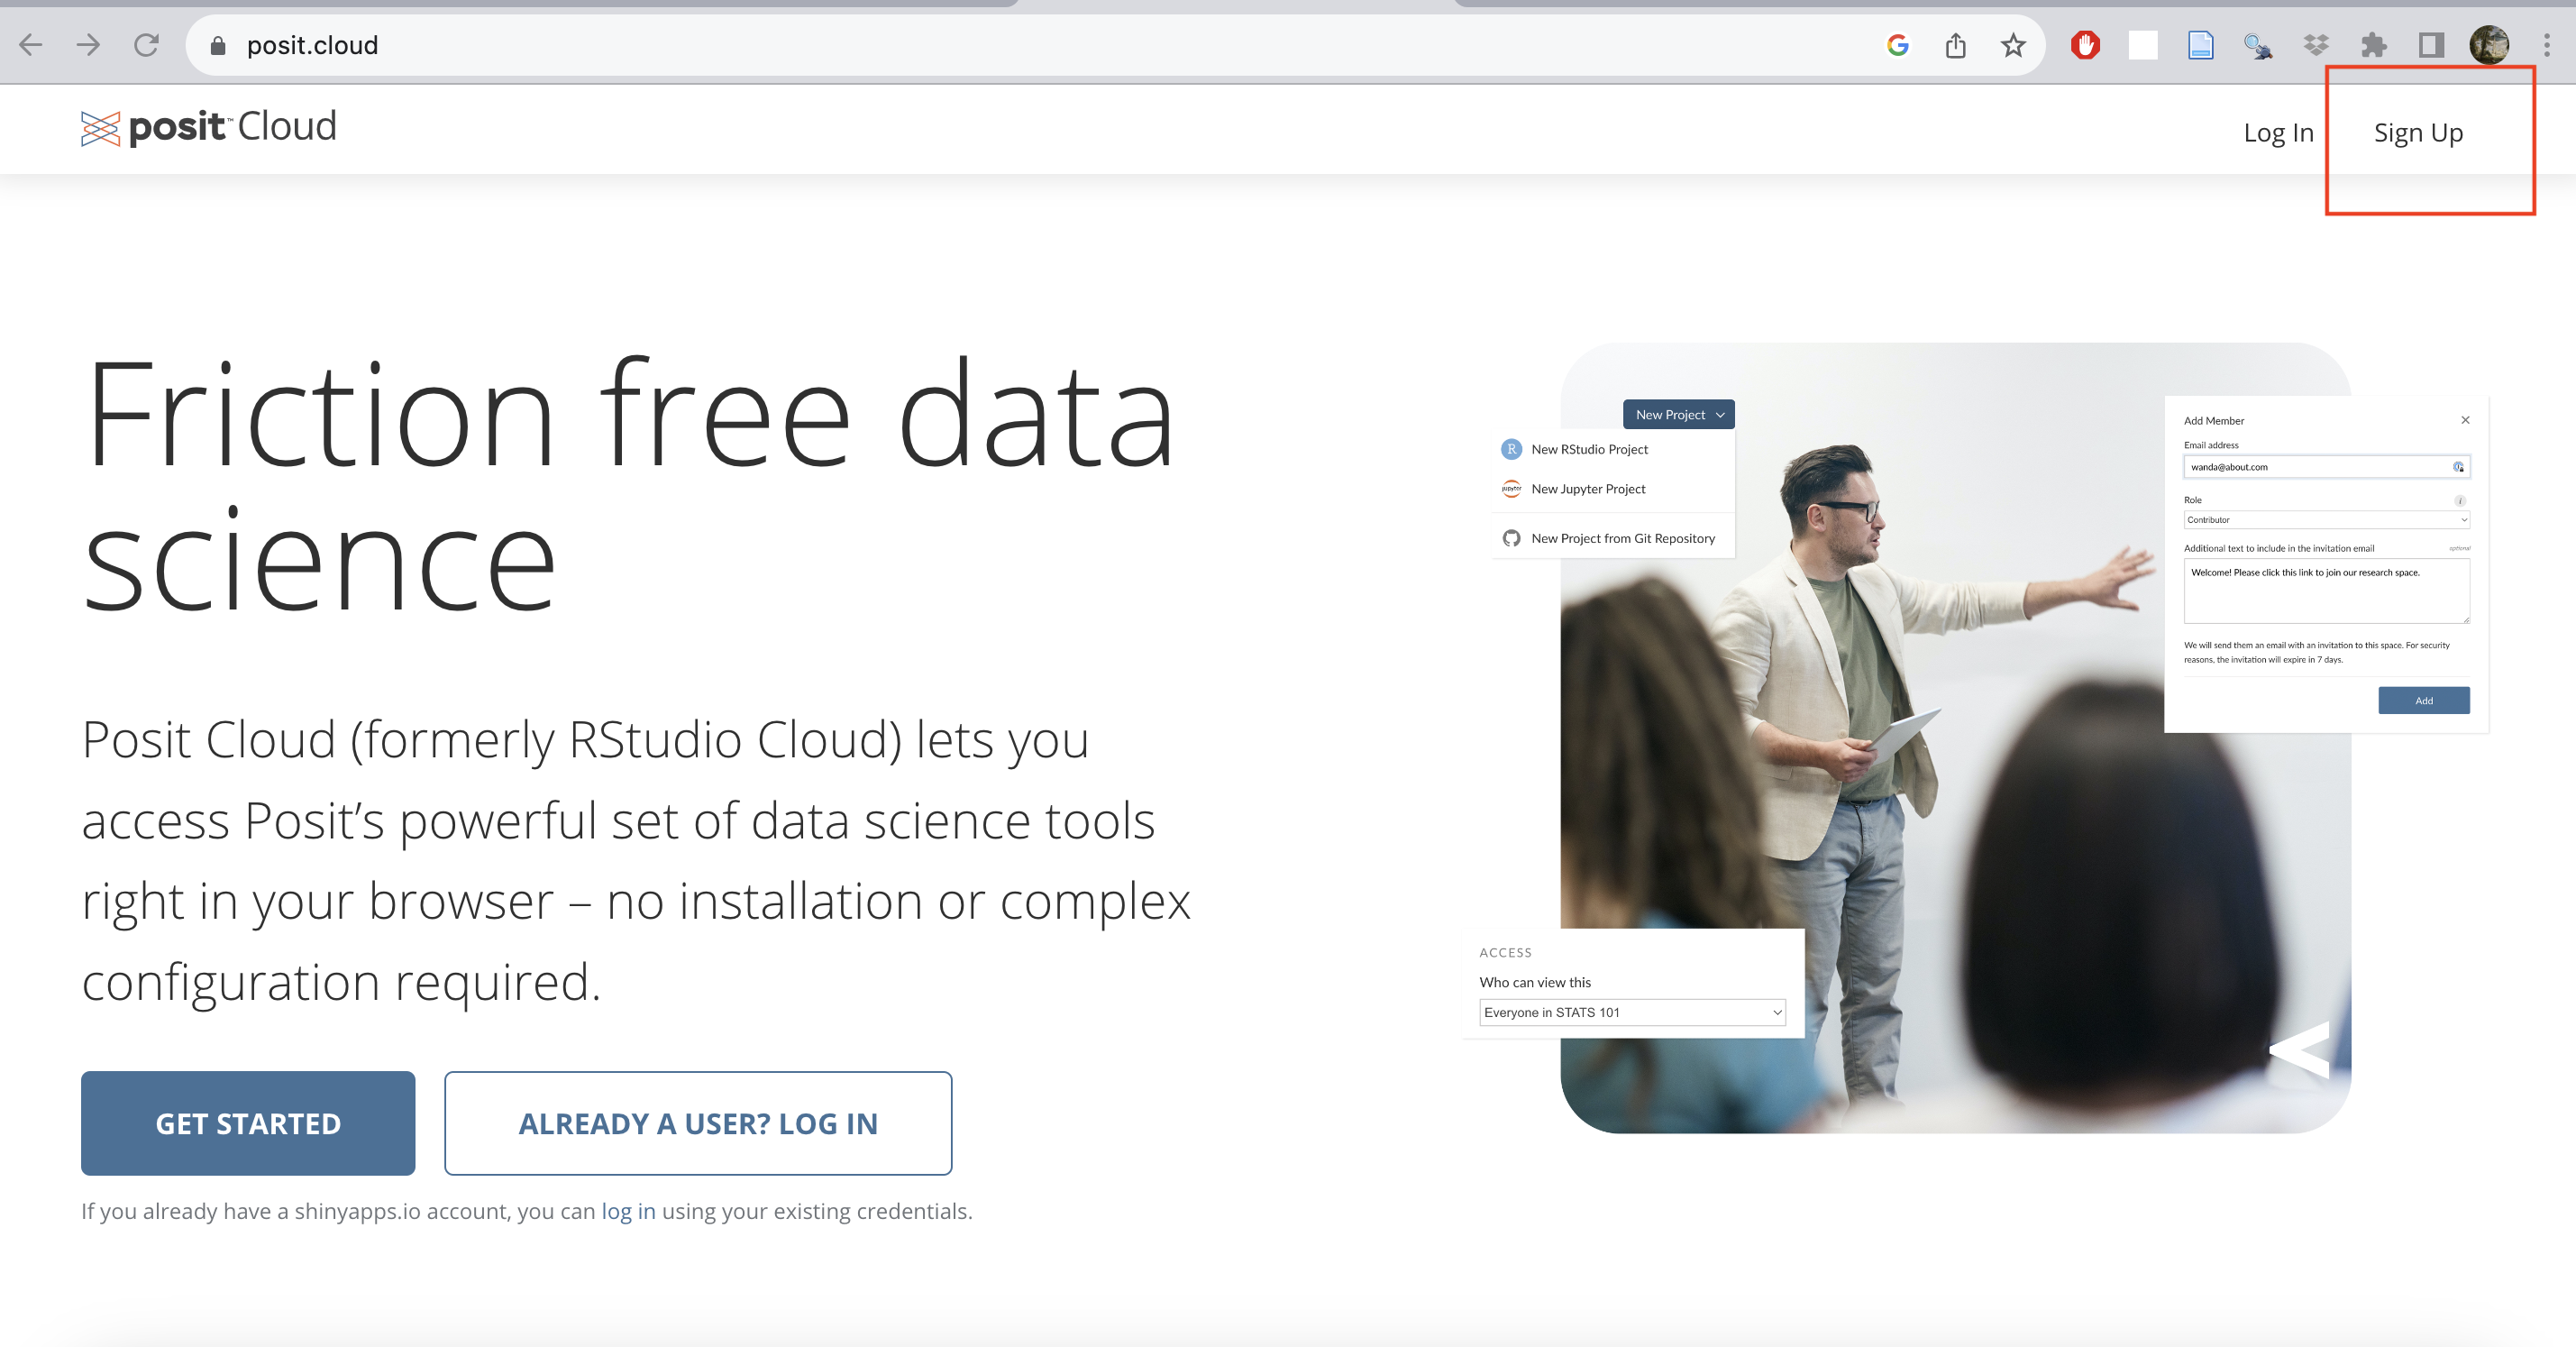
\includegraphics[keepaspectratio]{images/Screenshot 2023-08-25 at 12.36.55.png}}

Sign up to Posit cloud with an email address here:
\url{https://posit.cloud/plans}

Click on `Learn more' under the Free plan, and then `Sign up'.

Click on the invite link posted on Brightspace. Once you have signed up,
click on the `burger' icon to the left of `Your Workspace' to open a
sidebar, which will allow you to switch to the correct workspace
`Information Visualisation and the Humanities':

\pandocbounded{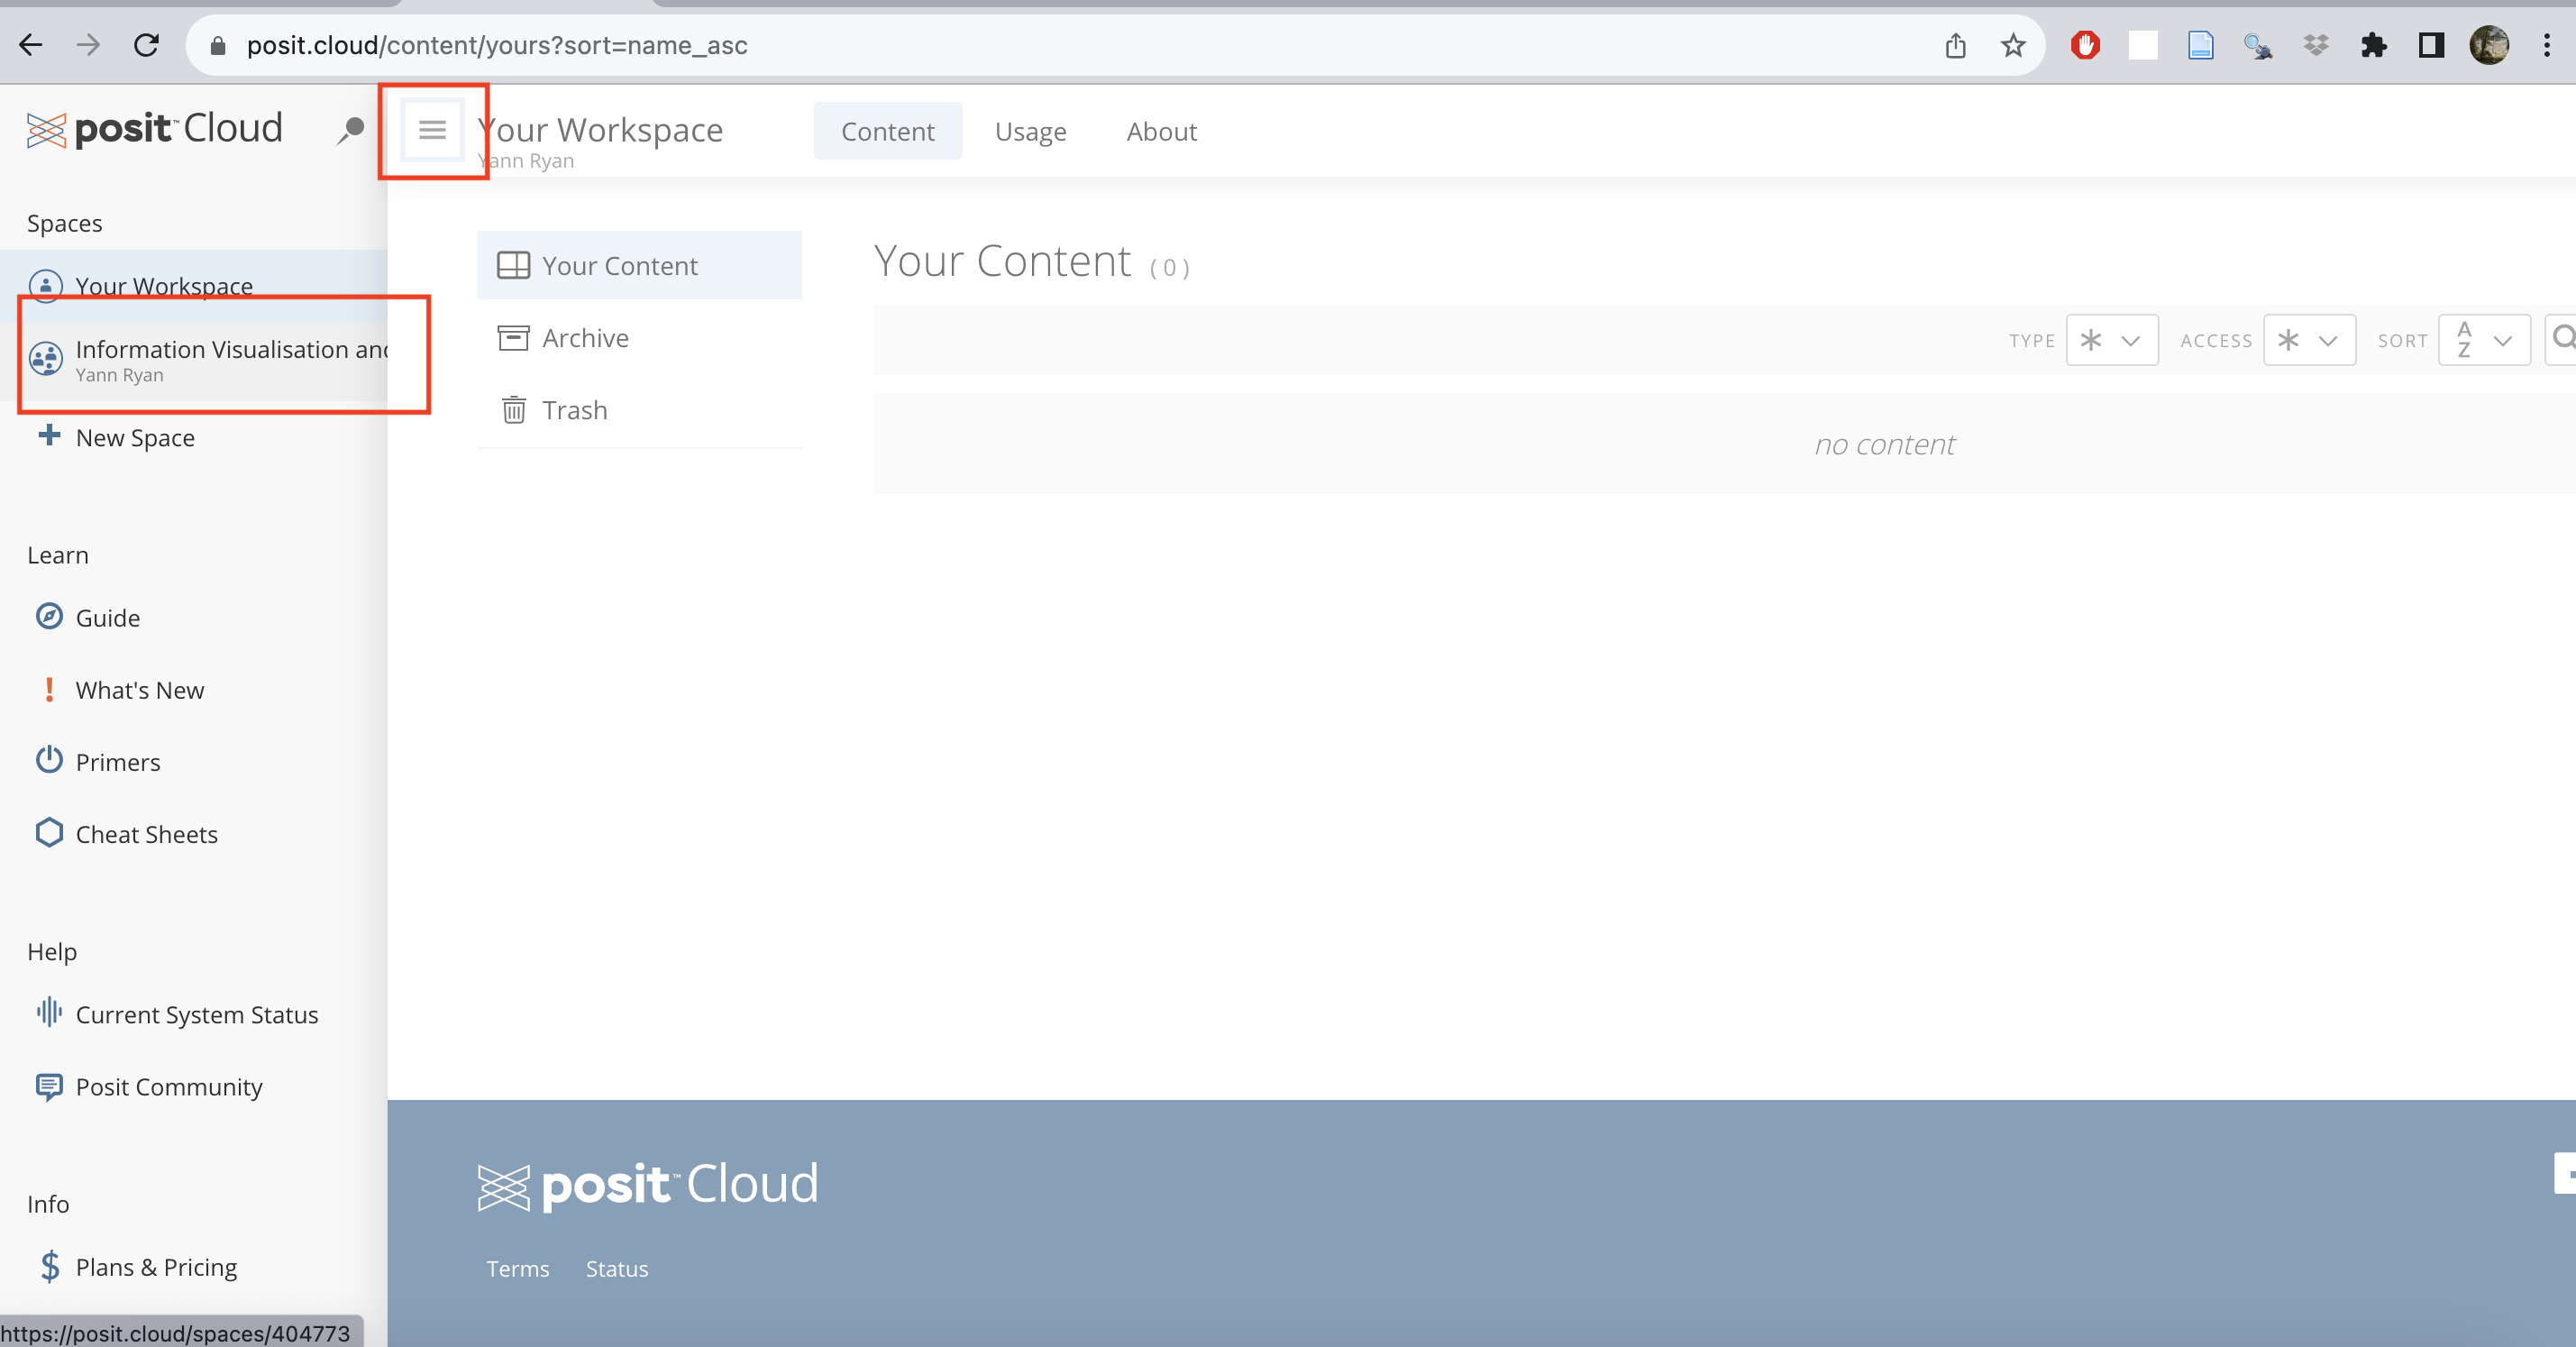
\includegraphics[keepaspectratio]{images/Screenshot 2023-08-25 at 12.49.30.png}}

Once you have switched, you'll see a list of assignments and projects.
At the moment, there is just one for this week. Click the start button
for `Week 1: Introduction'.

\pandocbounded{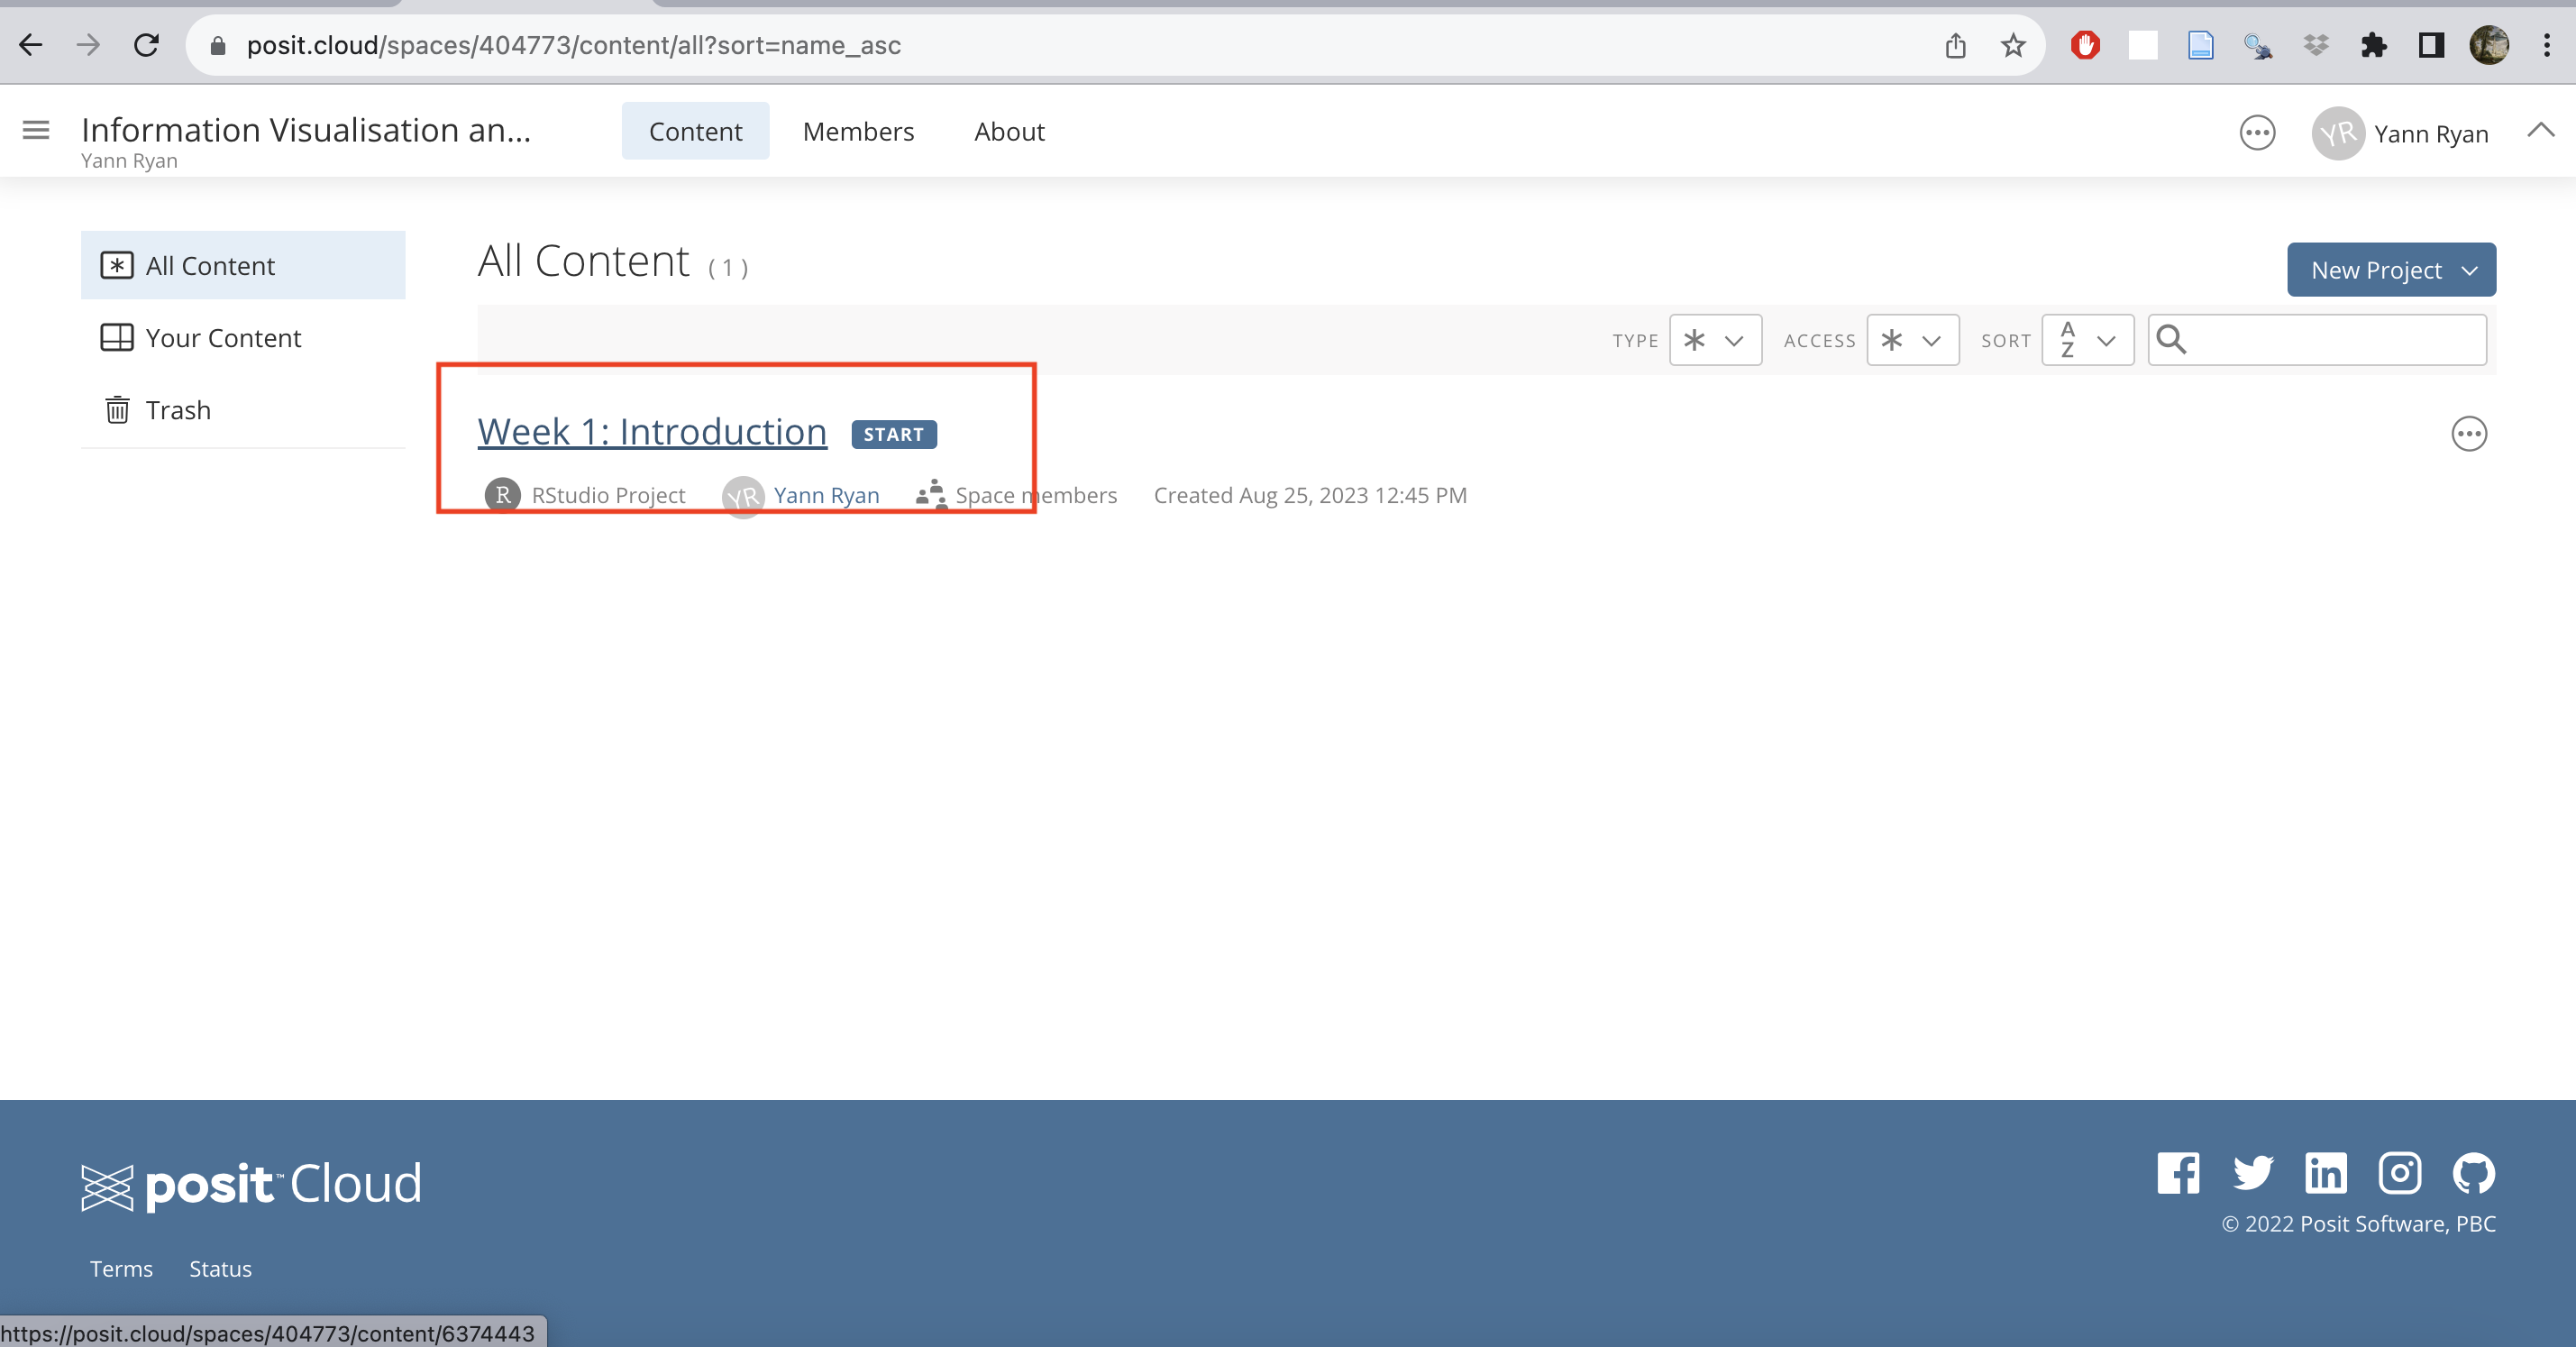
\includegraphics[keepaspectratio]{images/Screenshot 2023-08-25 at 12.50.09.png}}

This will load, and you should shortly be greeted with the Rstudio
interface -- this is an environment for creating and editing R code.

\pandocbounded{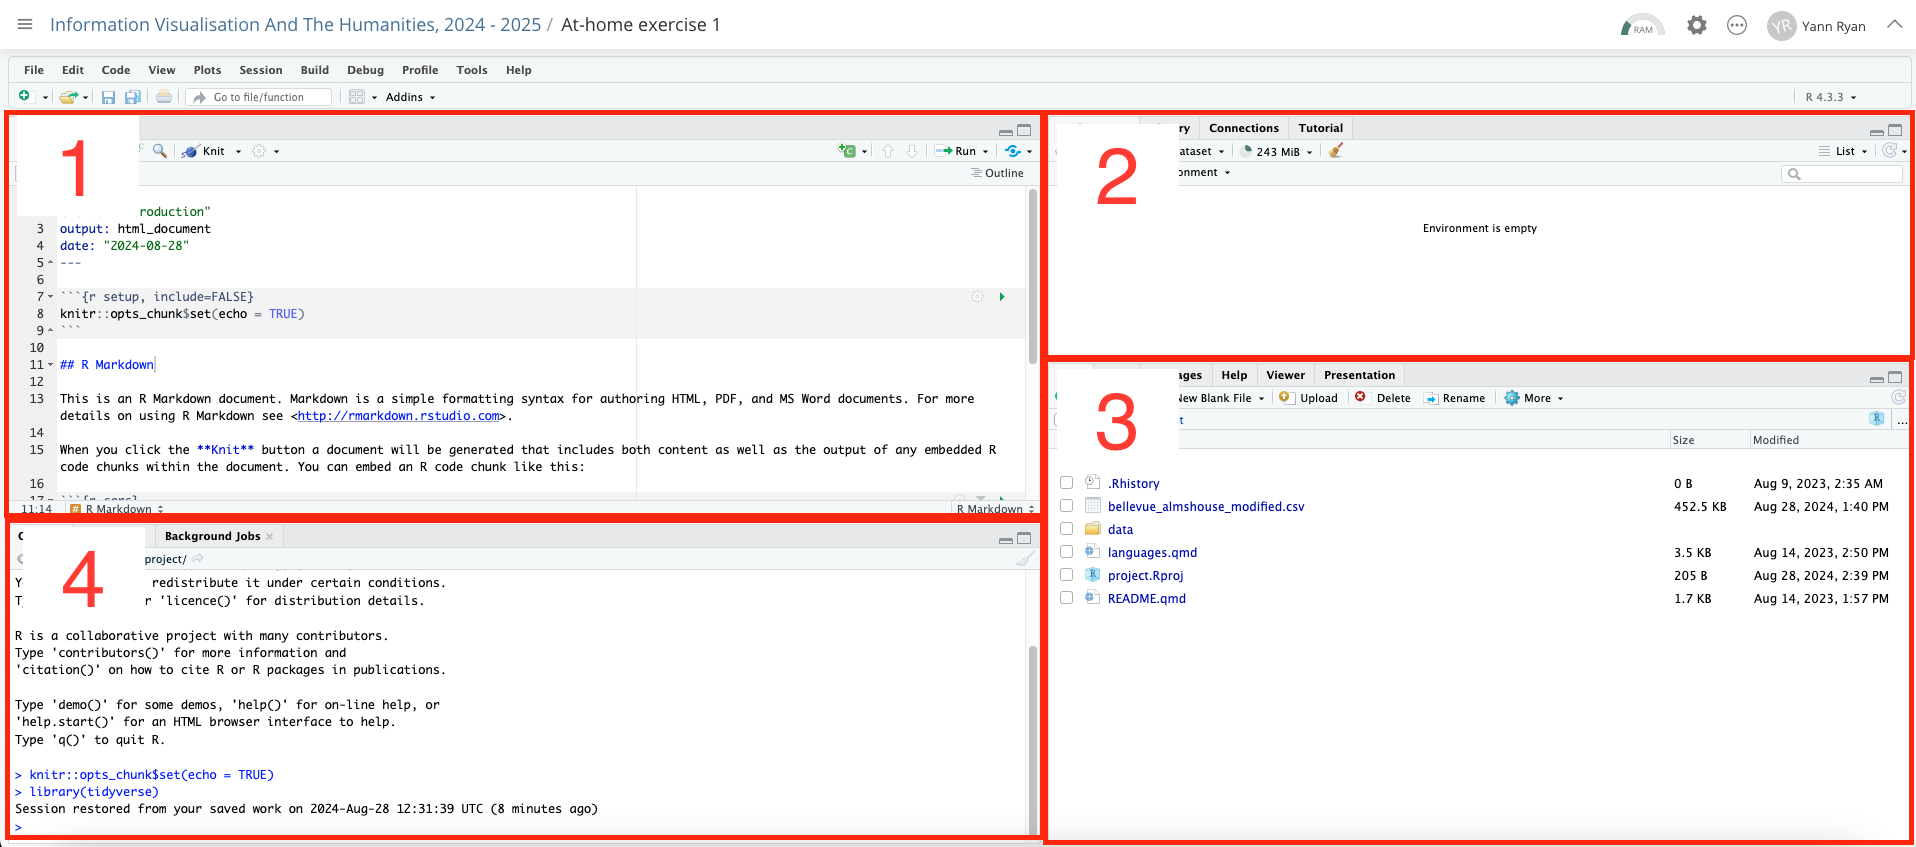
\includegraphics[keepaspectratio]{images/Screenshot 2024-08-28 at 14.41.18.png}}

R-Studio is divided into four different sections, or \emph{panes}. Each
of these also has multiple tabs. Starting from the top-left (numbered
1):

\begin{enumerate}
\def\labelenumi{\arabic{enumi}.}
\item
  The source editor. Here is where you can edit R files such as
  RMarkdown or scripts.
\item
  The environment pane will display any objects you create or import
  here, along with basic information on their type and size.
\item
  This pane has a number of tabs. The default is files, which will show
  all the files in the current folder. You can use this to import or
  export additional files to R-Studio from your local machine.
\item
  The console allows you to type and execute R commands directly: do
  this by typing here and pressing return.
\end{enumerate}

All four of these panes are important and worth it's worth exploring
more of the buttons and menu items. Throughout this course, you'll
complete exercises by using the source editor to edit notebooks. As you
execute code in these notebooks, you'll see objects pop into the
environment pane. The console can be useful to test code that you don't
want to keep in a document. Lastly, getting to know how to use and
navigate the directory structure using the files pane is essential.

You can play around with the R-Studio interface. Don't worry about
breaking anything, but you should regularly save your work.

\section{Your Derived Workspace}\label{your-derived-workspace}

You can return to the workspace overview by clicking on the sidebar and
on the `Information Visualization{[}\ldots{]}' menu item again.

If you do this, you'll see that there are now \emph{two} workspace
items. This is because when you started the workspace, it created a
`derived' version - meaning it has created a unique copy for you to work
with, without changing the original one.

You can delete this version, copy it, or export a copy to your local
machine. When you want to resume your work, you should open this copy.
\textbf{Please note that as the instructor, I can see and edit all the
derived workspaces.}

\pandocbounded{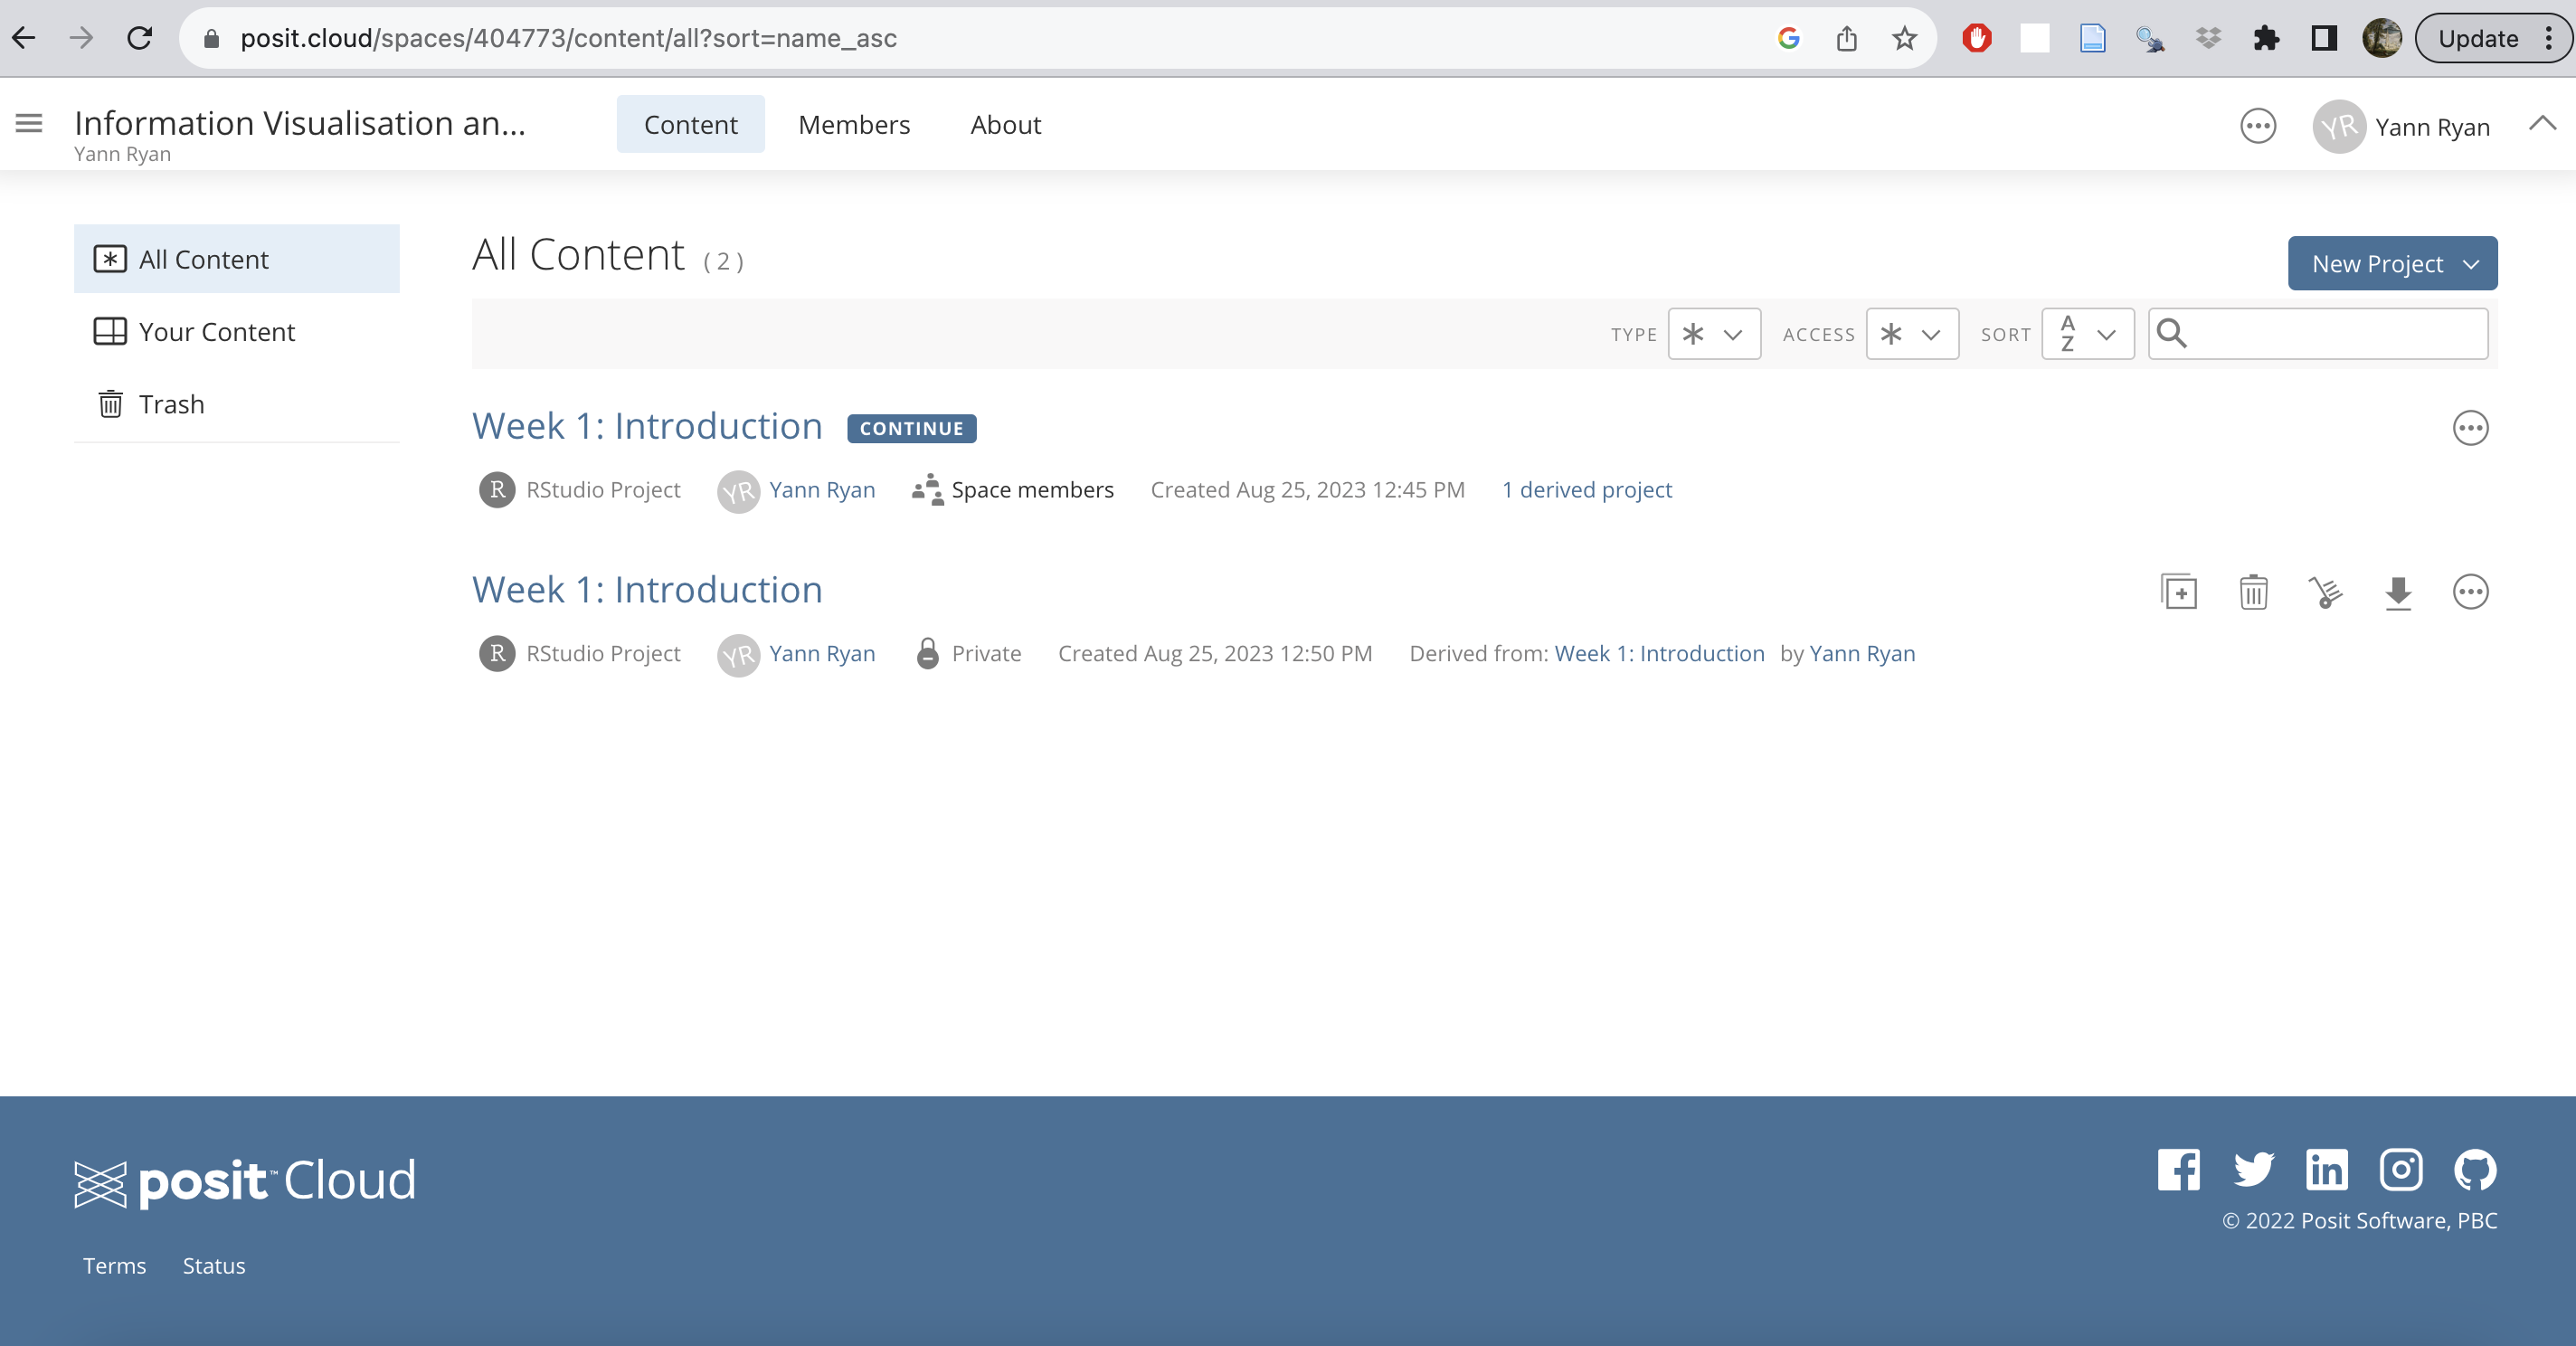
\includegraphics[keepaspectratio]{images/Screenshot 2023-08-28 at 13.48.01.png}}

\section{R Markdown and `Knitting' a
Document}\label{r-markdown-and-knitting-a-document}

There are several ways to create and execute code within R studio, such
as creating scripts or typing into the console (the bottom-left pane).

However, in this course, we'll exclusively use one method: R Markdown
notebooks.

These are special documents which can include code and text. Text is
written using a simple format called Markdown, and code goes into
special `cells' within the document. Once you're finished, you'll tell R
studio to execute all the code in the document and render it as an html
file. This process is called `knitting'.

We'll worry more about code next week, but for now, let's just get used
to creating R Markdown files, knitting them, and downloading them to
your local machine so they can be sent as assignments.

\subsection{Create a new markdown
file}\label{create-a-new-markdown-file}

Click file -\textgreater{} new file -\textgreater{} R notebook.

\pandocbounded{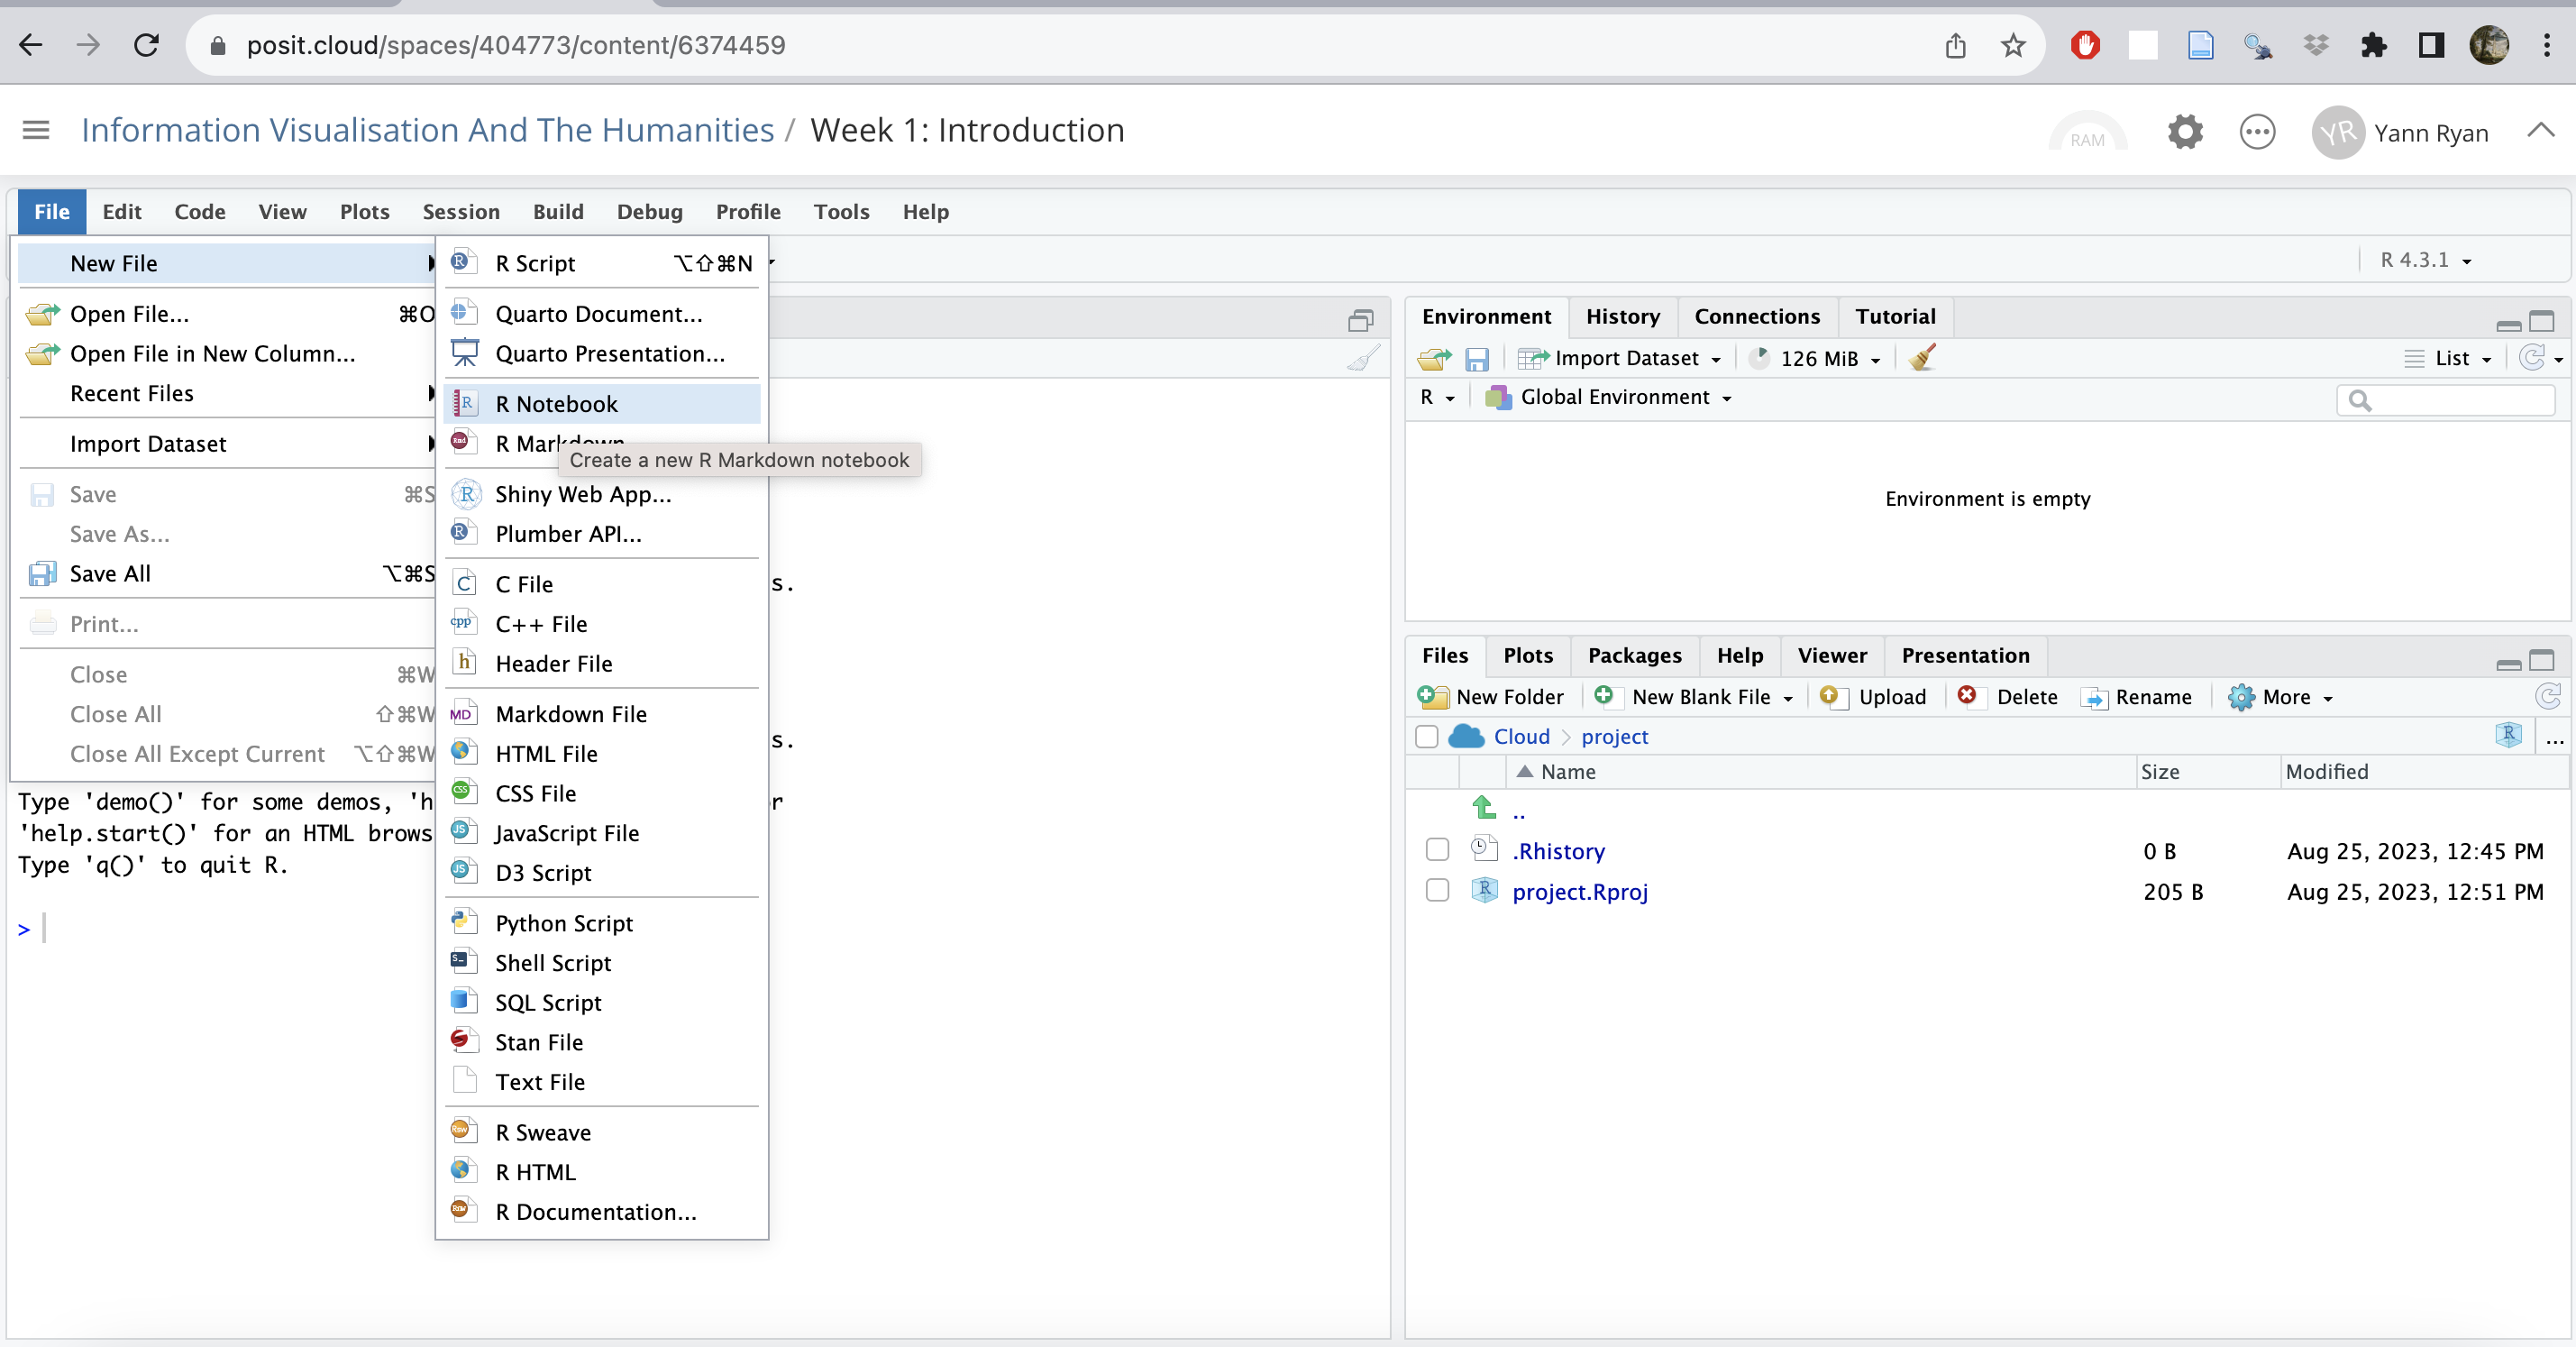
\includegraphics[keepaspectratio]{images/Screenshot 2023-08-25 at 12.51.20.png}}

This will open a markdown notebook in the top-left pane. If asked to
install packages, just click yes, and wait a little longer.

A notebook will now be open in your screen. This is where you can type
text and code.

At the moment, there is some sample text and code in the document.

At the top of the document is some formatted text which looks like this:

\pandocbounded{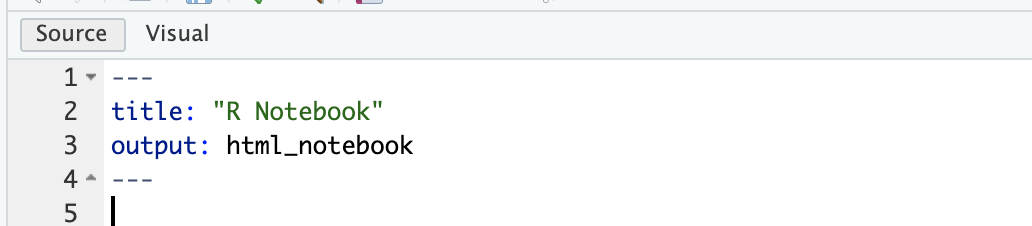
\includegraphics[keepaspectratio]{images/Screenshot 2023-08-25 at 12.53.35.png}}

This is called a yaml header. It contains information about your
document, and it needs to remain here for the notebook to work. You can
use this yaml header to edit the title of your report: just edit the
text within the quotation marks which now reads `R Notebook'.

You should delete the rest of the text in the document: highlight and
delete the rest of the contents of the notebook, using delete/backspace.

\subsection{Type some text}\label{type-some-text}

Type some text. There are two ways of doing this. You can use the source
editor, which is the default view. You can switch between Source and
Visual using the button above.

\pandocbounded{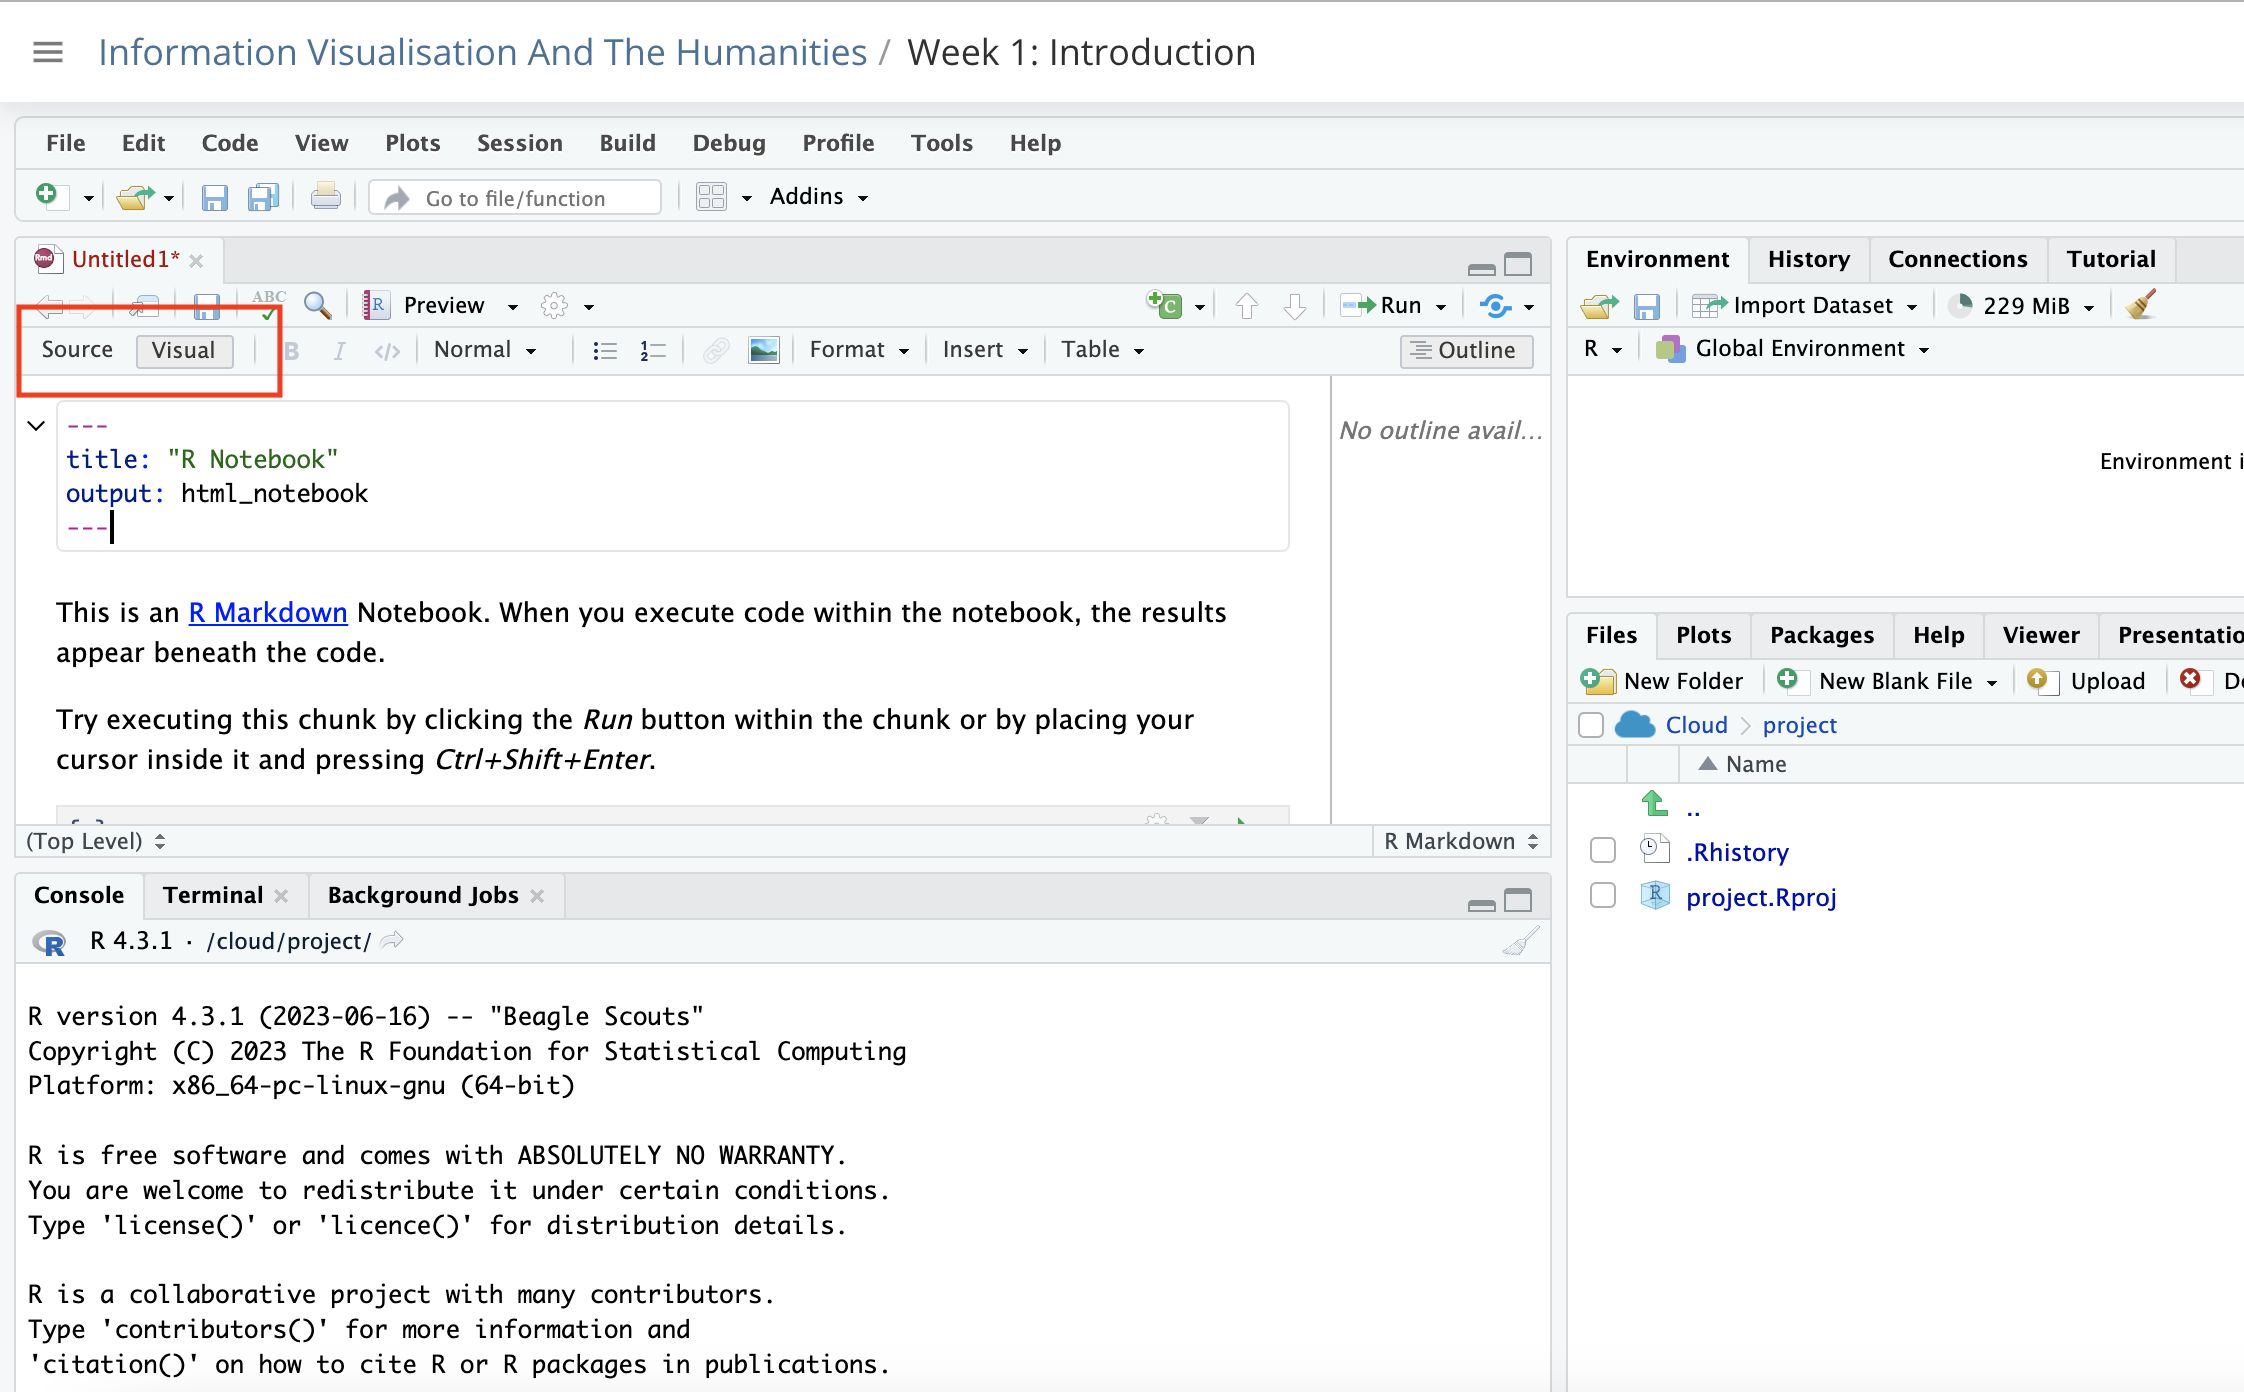
\includegraphics[keepaspectratio]{images/Screenshot 2023-08-25 at 12.55.20.png}}

In the source editor, use markdown. This is a very simple coding
language used to render text on the internet. There are codes for bold,
italics, headings. You can add images etc. You can switch between the
two at any time.

\pandocbounded{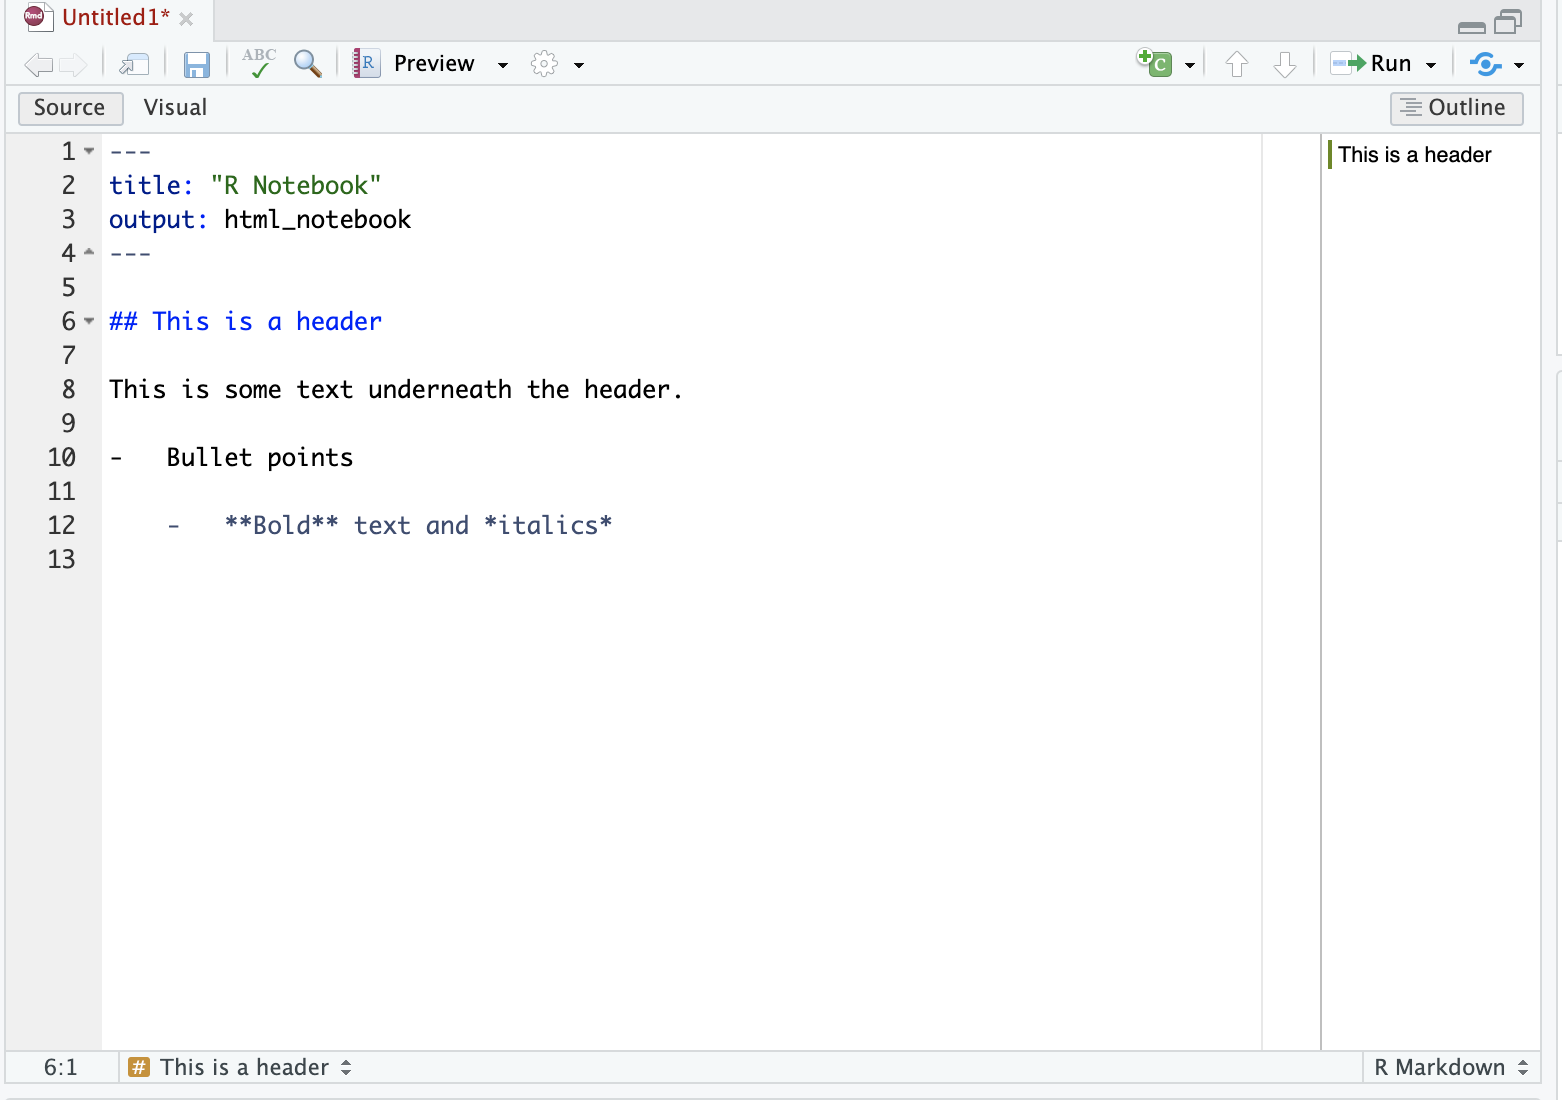
\includegraphics[keepaspectratio]{images/Screenshot 2023-08-25 at 12.56.52.png}}

In the visual editor, use the menu items to format your text. For
example bold, italics, headings. You can use the drop-down menu to add
images, tables, and so forth, as you would with word processor software
such as Word or Google docs.

\pandocbounded{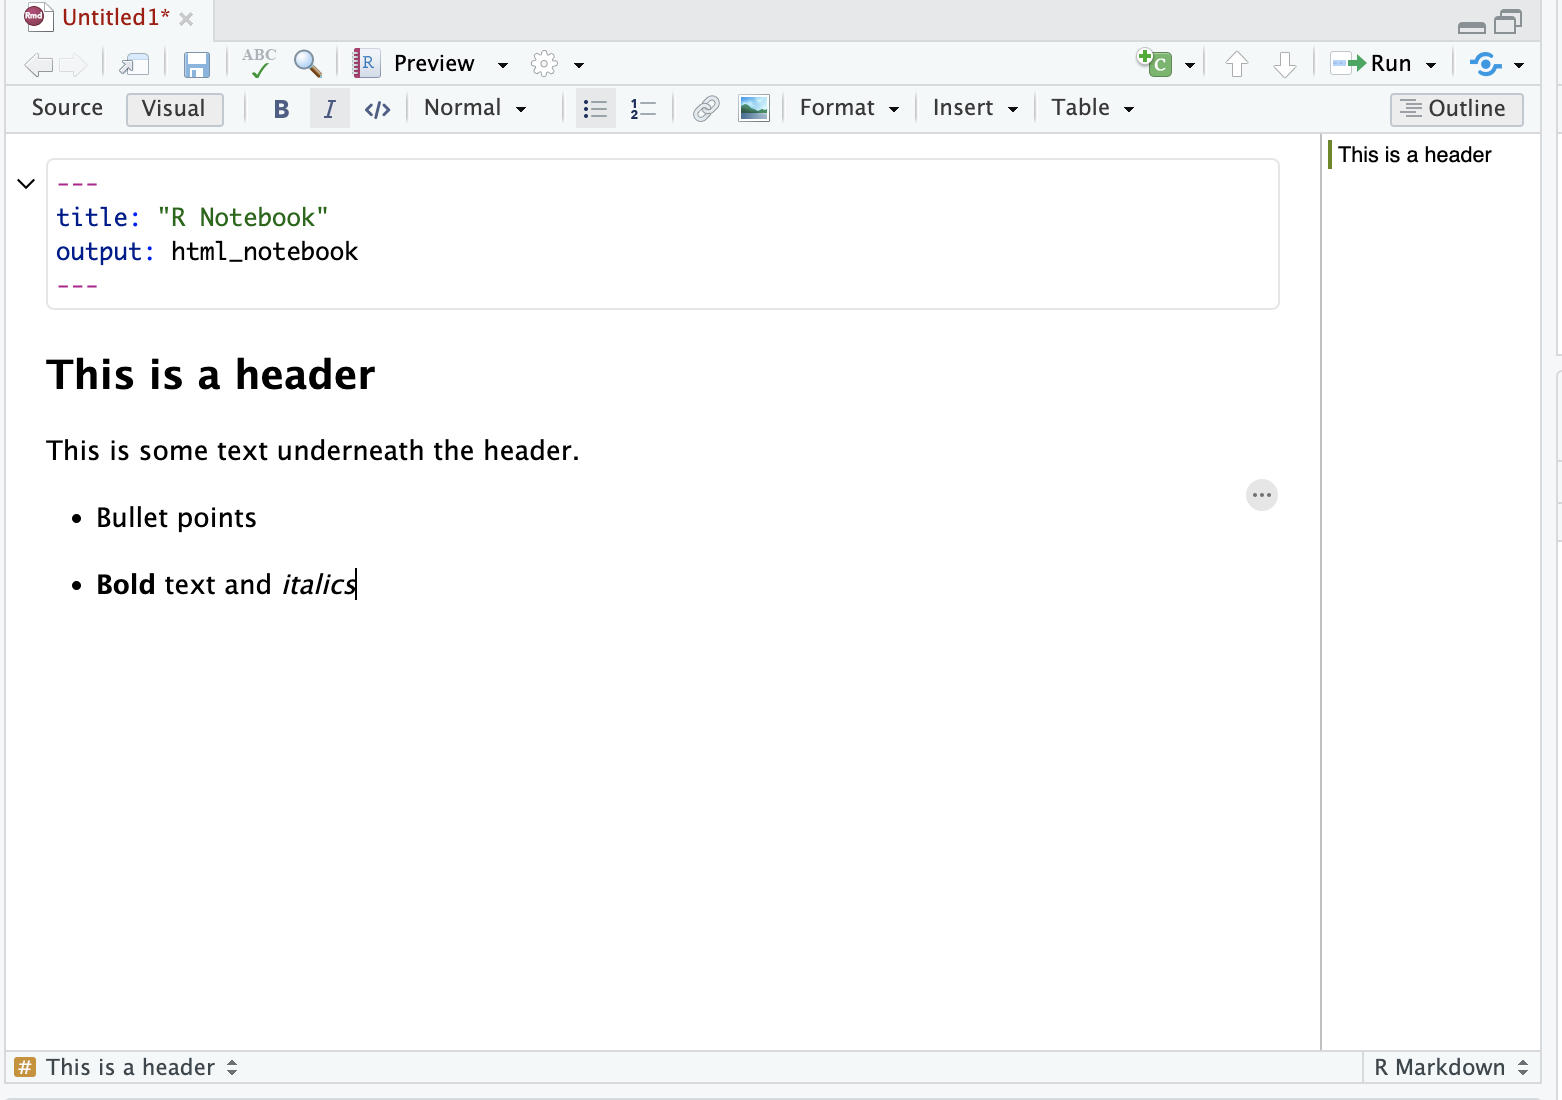
\includegraphics[keepaspectratio]{images/Screenshot 2023-08-25 at 12.56.33.png}}

\begin{tcolorbox}[enhanced jigsaw, coltitle=black, bottomrule=.15mm, title=\textcolor{quarto-callout-warning-color}{\faExclamationTriangle}\hspace{0.5em}{Warning}, leftrule=.75mm, colframe=quarto-callout-warning-color-frame, breakable, toprule=.15mm, opacityback=0, bottomtitle=1mm, toptitle=1mm, colback=white, rightrule=.15mm, titlerule=0mm, left=2mm, arc=.35mm, opacitybacktitle=0.6, colbacktitle=quarto-callout-warning-color!10!white]

Be careful when switching between the Source and Visual editors, as this
is an easy way to get weird formatting errors. A common example of this
is accidentally adding the markdown code for a title (e.g \texttt{\#\#})
in the Visual mode instead of the Source mode.

\end{tcolorbox}

\subsection{Save the file}\label{save-the-file}

In order to render/knit the file, it needs to be saved first.

Click file, save, and give it a name.

\pandocbounded{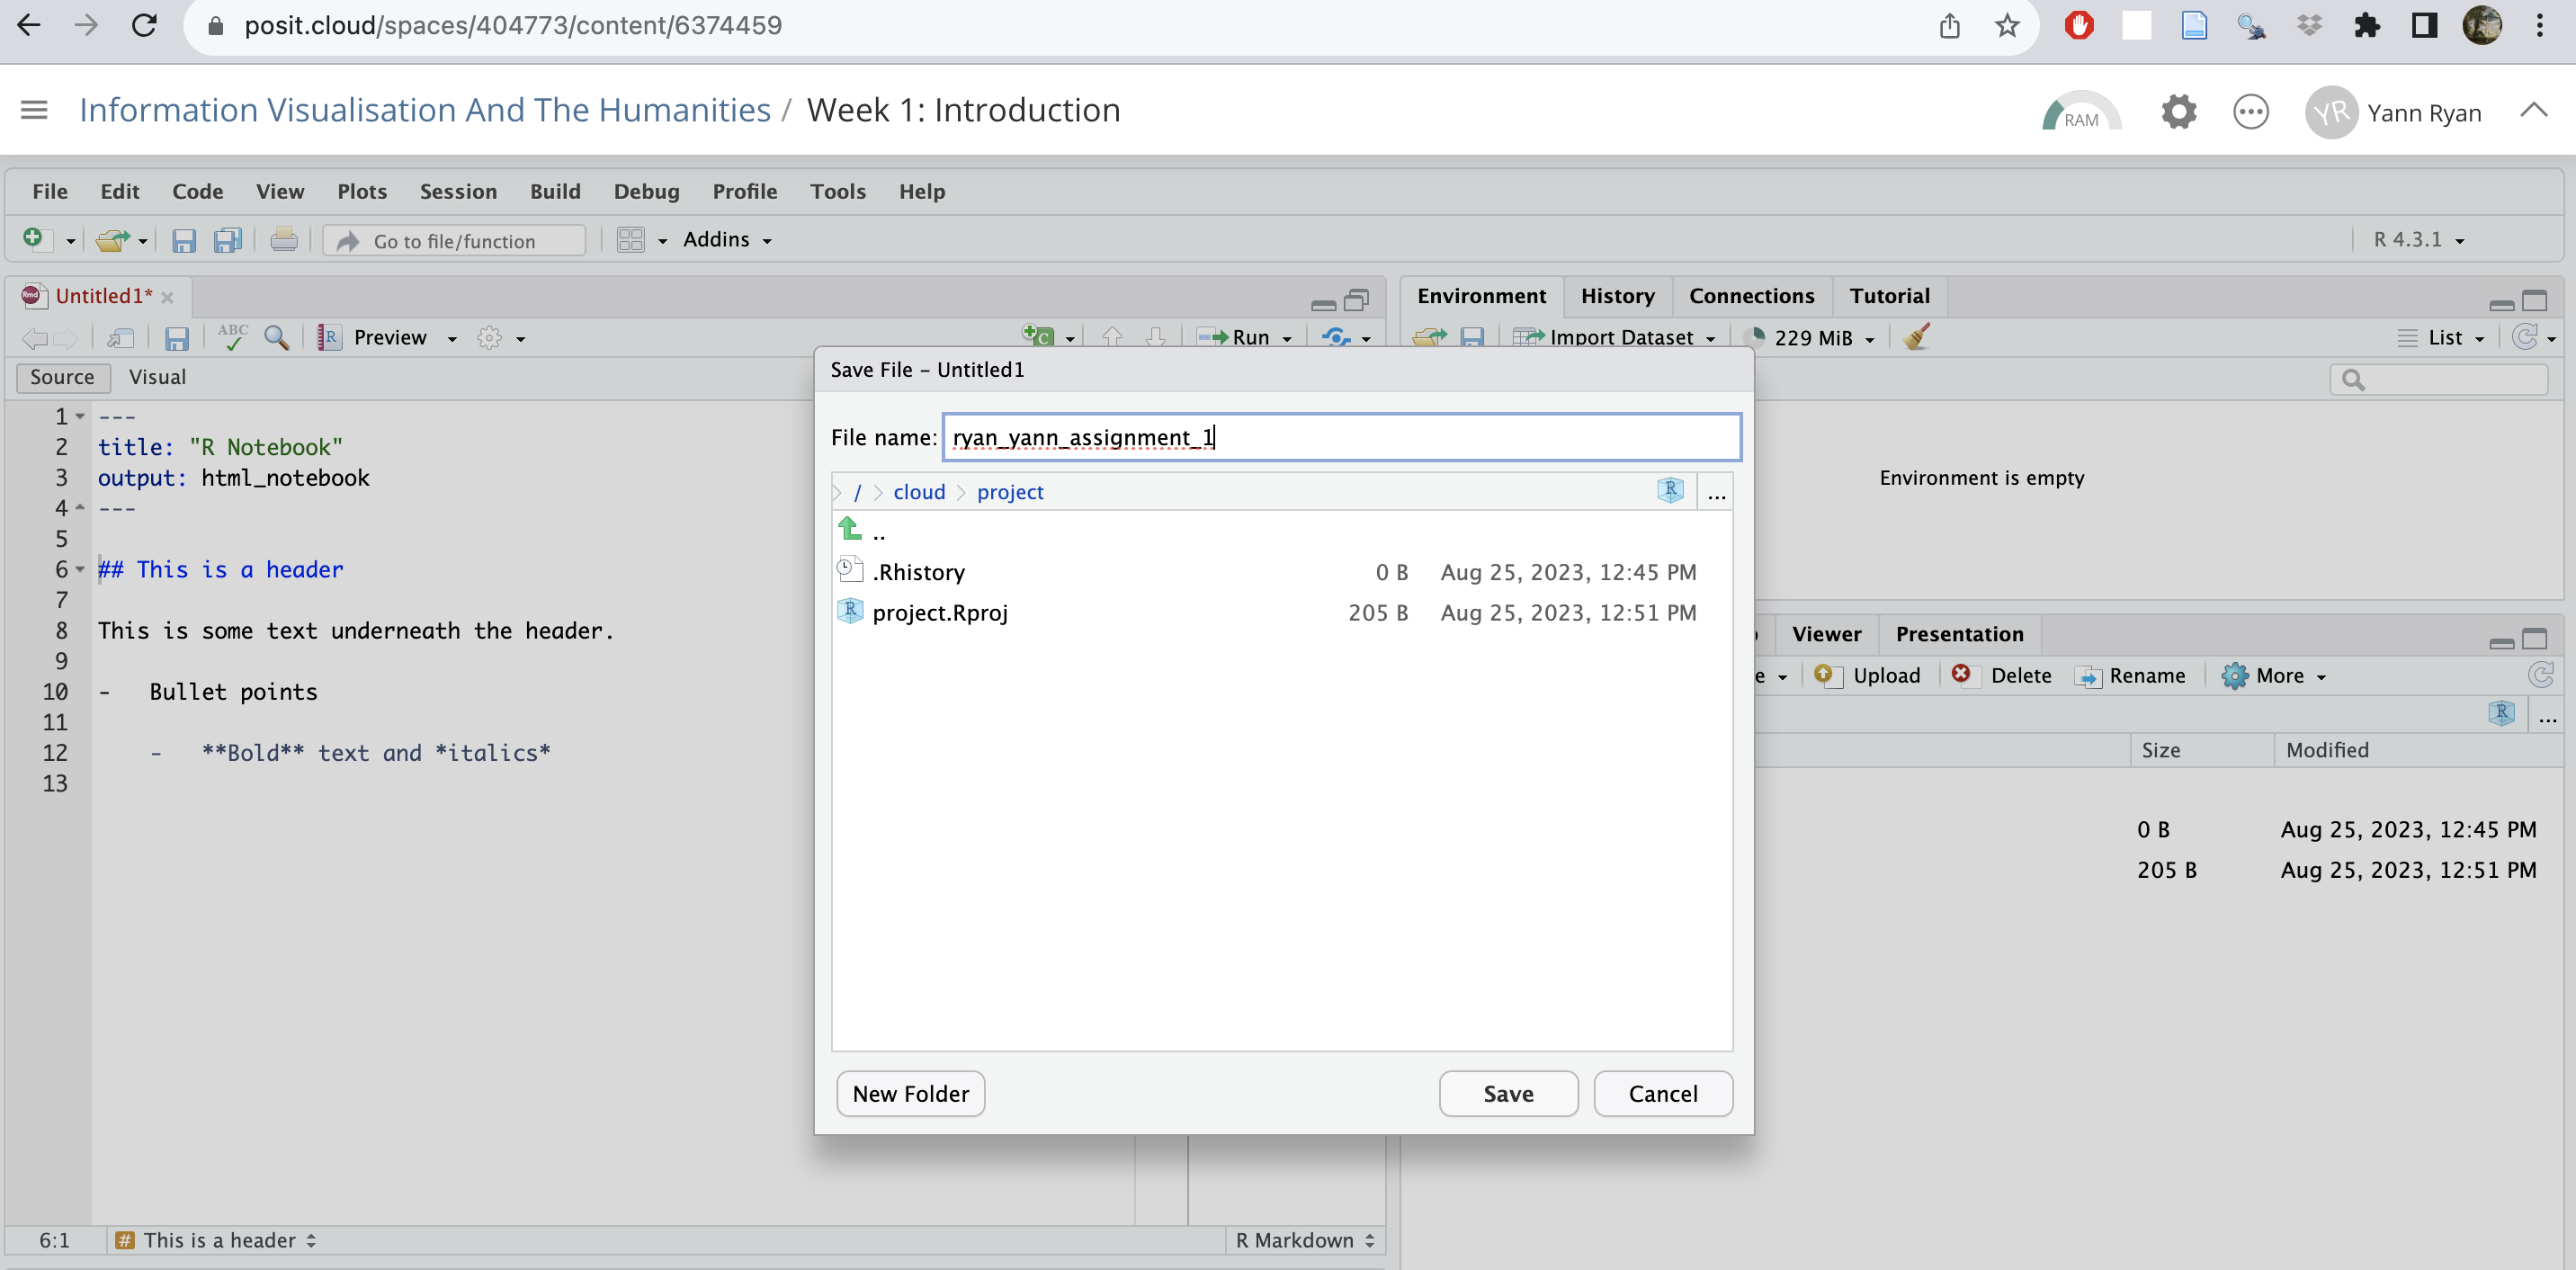
\includegraphics[keepaspectratio]{images/Screenshot 2023-08-25 at 12.57.40.png}}

\subsubsection{Naming conventions.}\label{naming-conventions.}

In this course, you will be required to use good naming conventions.
Save the file with an appropriate name which communicates the most
important information about the file: who created it, and what it
contains.

Once you have done this, you'll see a new .Rmd file appear in the file
browser, in the bottom-right pane:

\pandocbounded{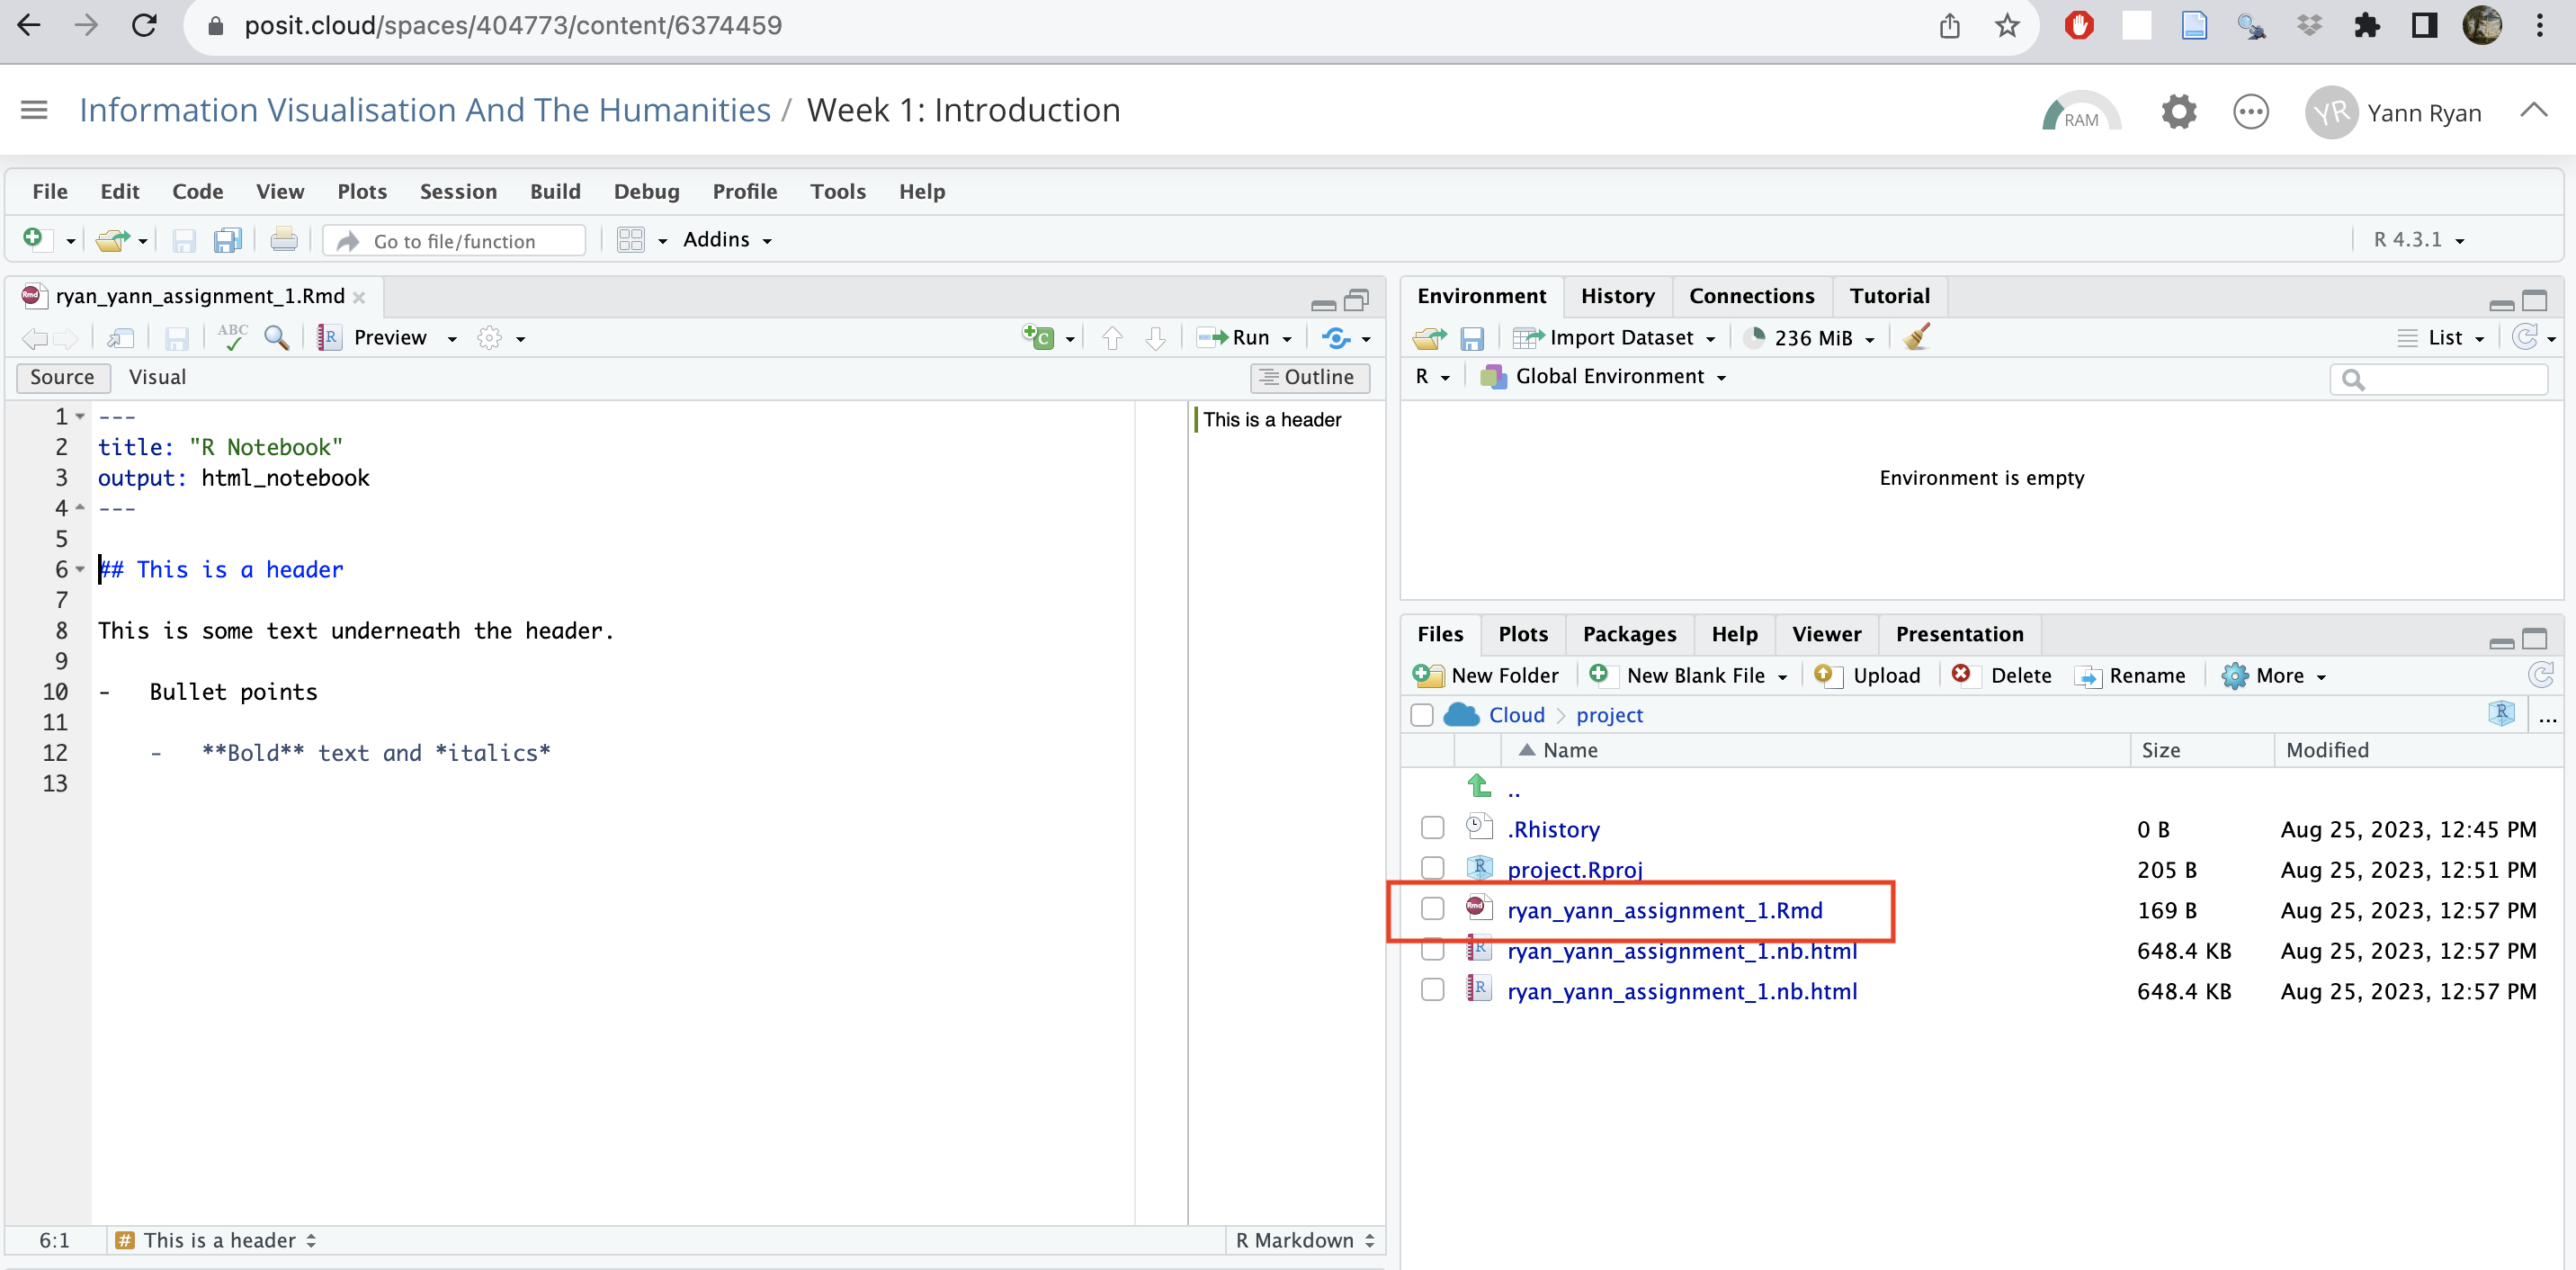
\includegraphics[keepaspectratio]{images/Screenshot 2023-08-25 at 12.58.28.png}}

\subsection{Knit the document}\label{knit-the-document}

Now, we'll render the document. When a document is rendered, it restarts
the R engine, runs through the code, and outputs the document. In this
case, it will be very quick, as we haven't written any code.

Click the drop-down where it currently says `Preview', and then `render
HTML'. This will create a new file in your folder.

\pandocbounded{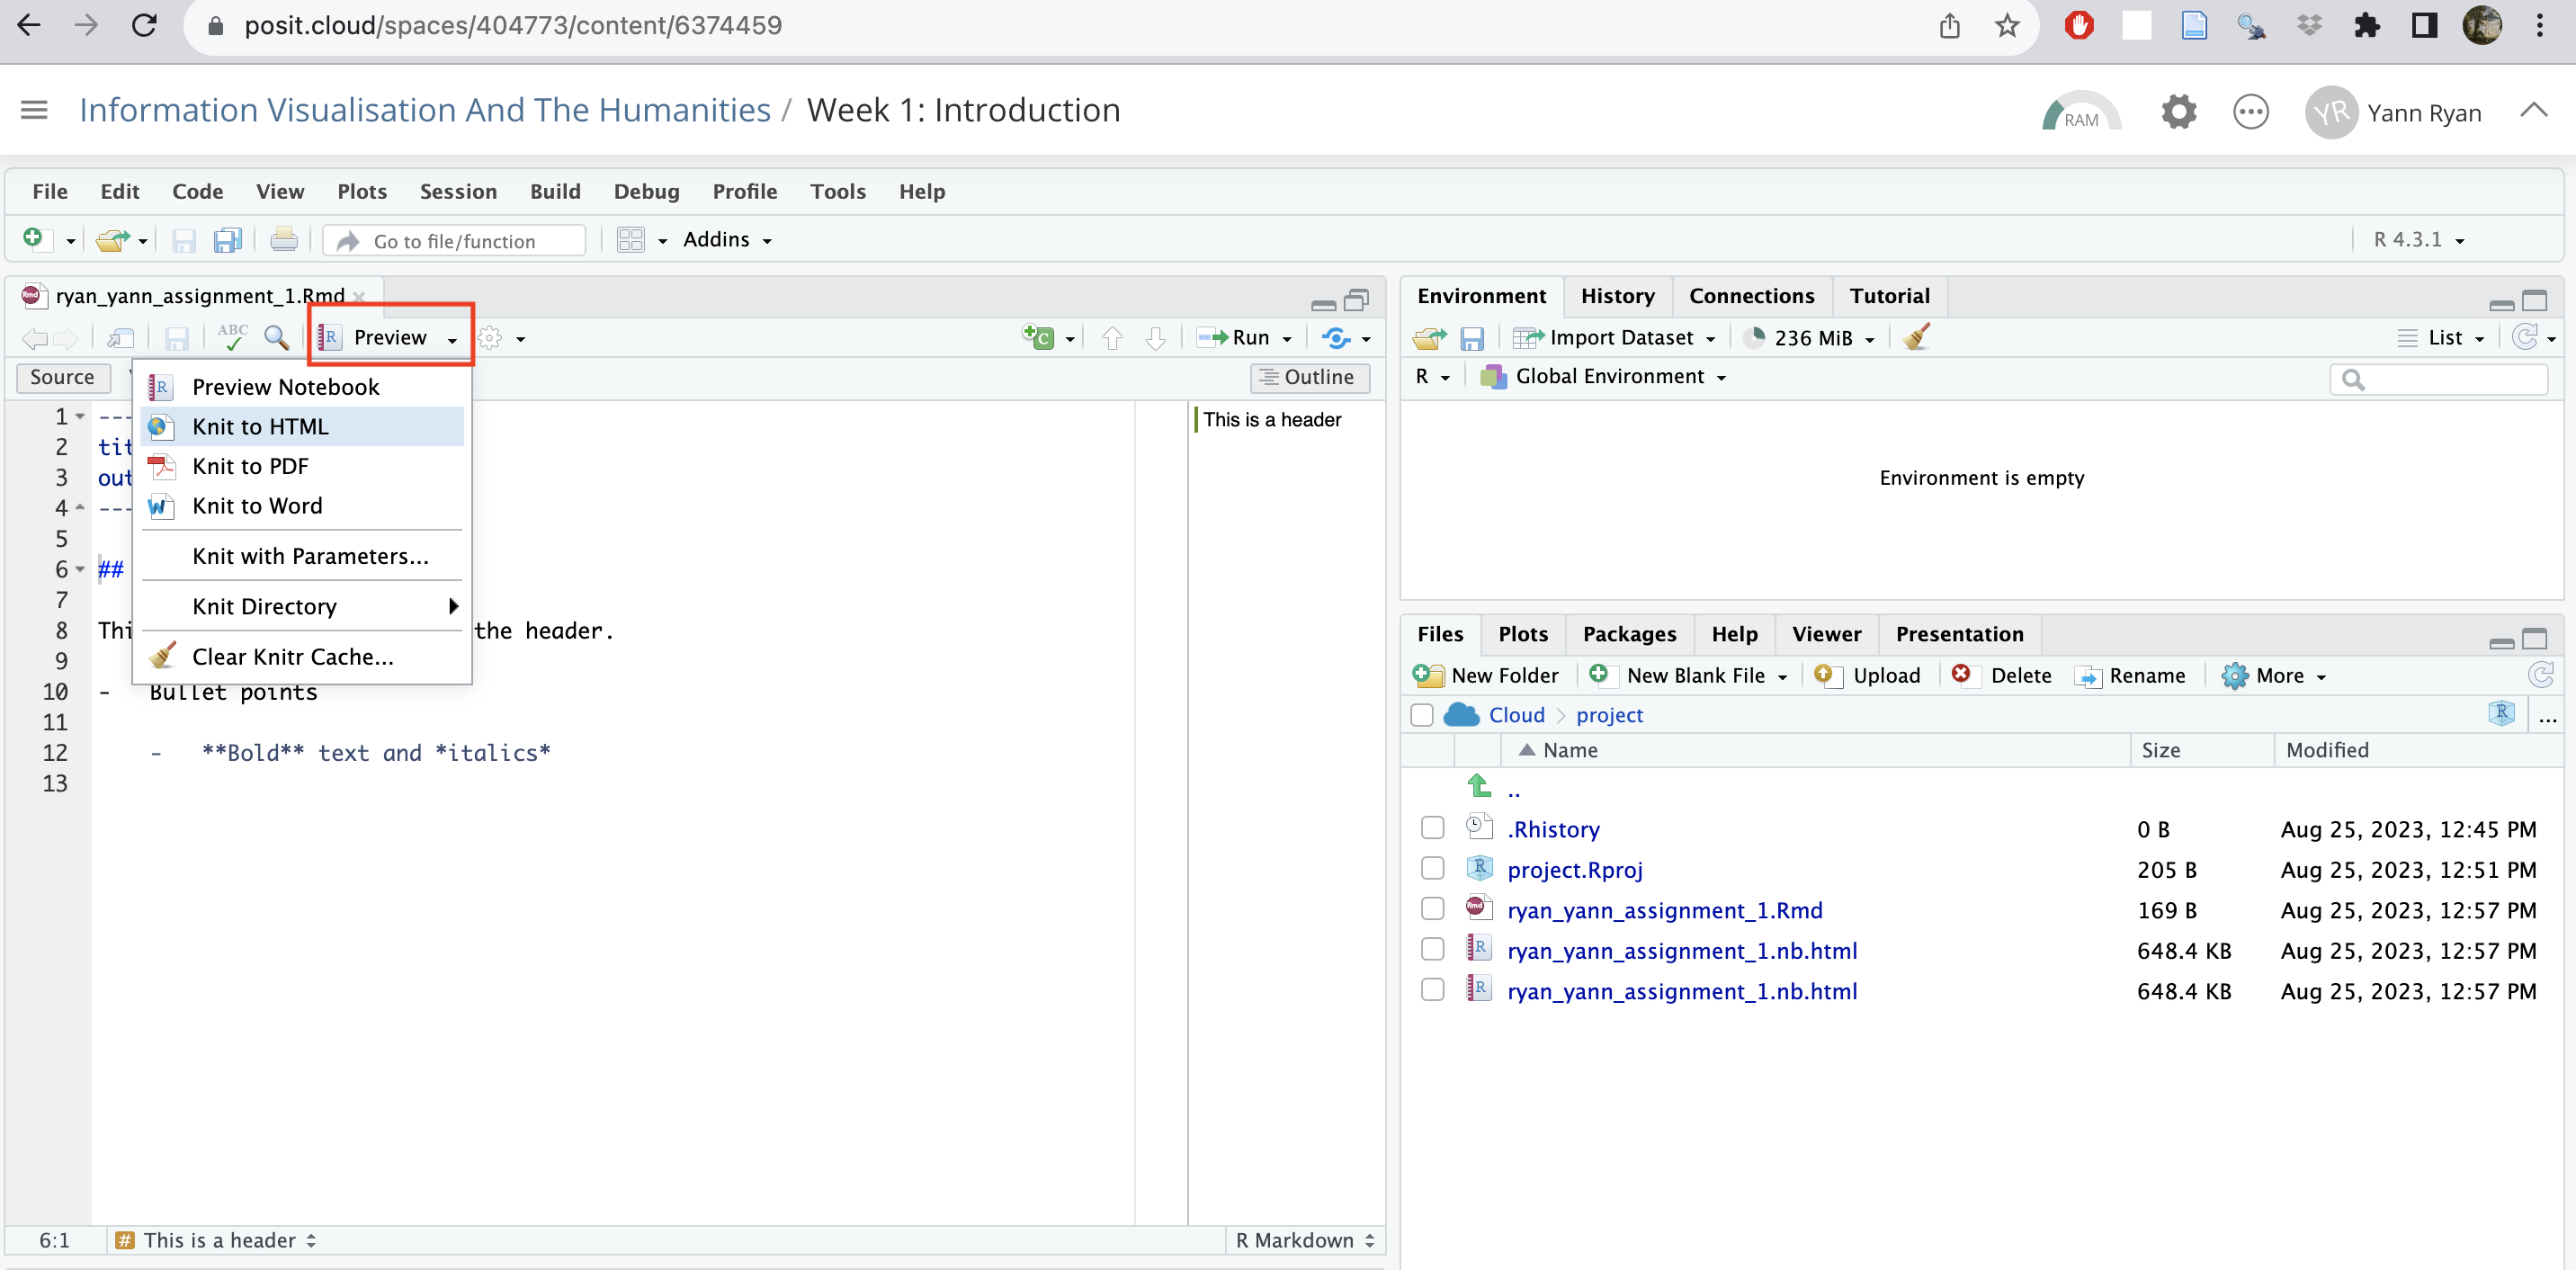
\includegraphics[keepaspectratio]{images/Screenshot 2023-08-25 at 12.59.37.png}}

The knitted html file will preview in a new window. You can close this.

More importantly, there are now a total of three additional files in the
file browser:

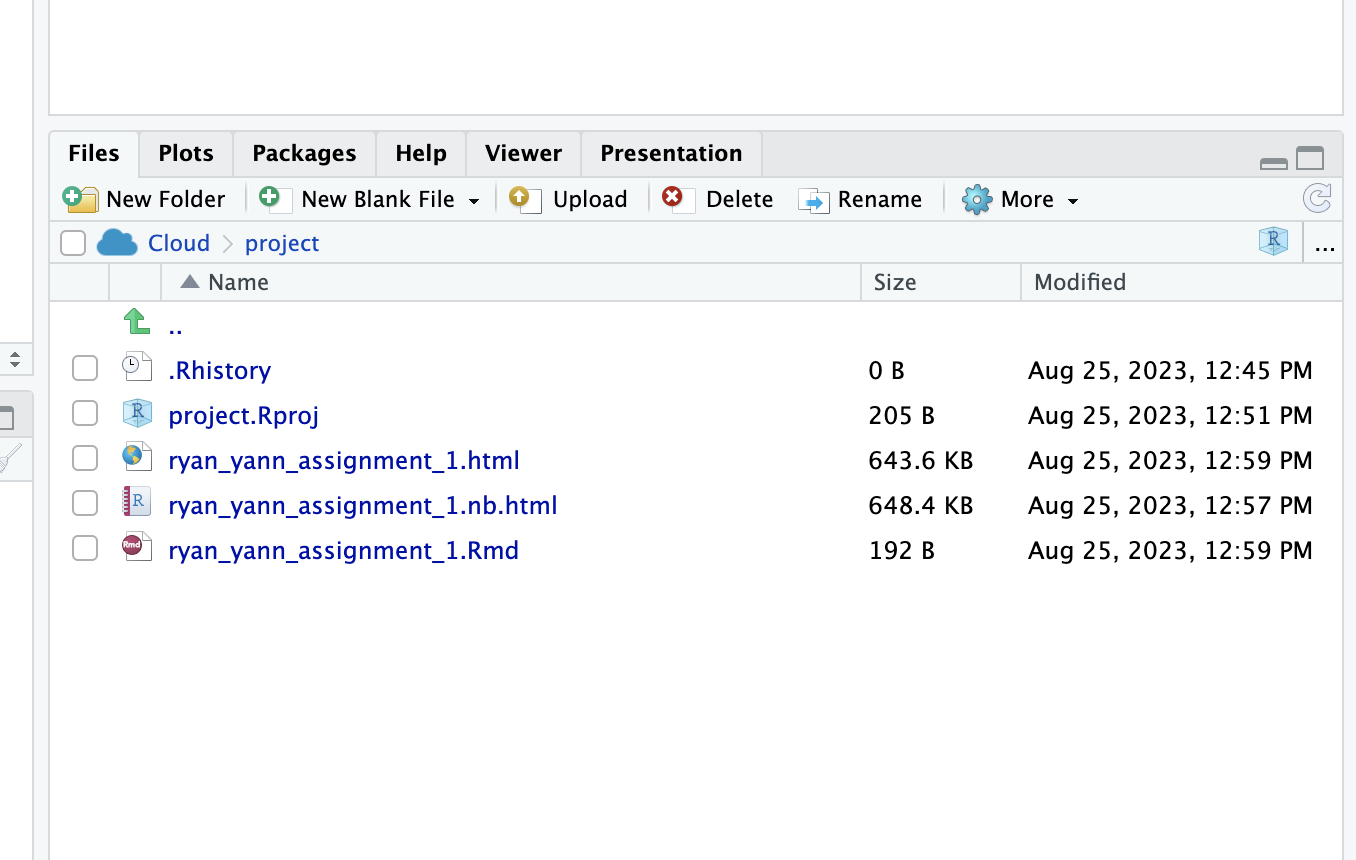
\includegraphics[width=6.25in,height=\textheight,keepaspectratio]{images/Screenshot 2023-08-25 at 13.00.52.png}

\begin{itemize}
\item
  The file ending in .html is the knitted output of the markdown.
\item
  The file ending in .Rmd is the `source code' of the final file.
\item
  The file ending in nb.html is created for making a quick preview, and
  can be ignored.
\end{itemize}

\subsection{Download and save the
file}\label{download-and-save-the-file}

To submit R Markdown files as assignments in Brightspace, you'll need to
download both the html output and the `raw' markdown file to your local
machine, and turn them both into a .zip file first.

Click on the checkbox for both the html and the .Rmd file.

Click on the `More' dropdown menu, and then `Export'

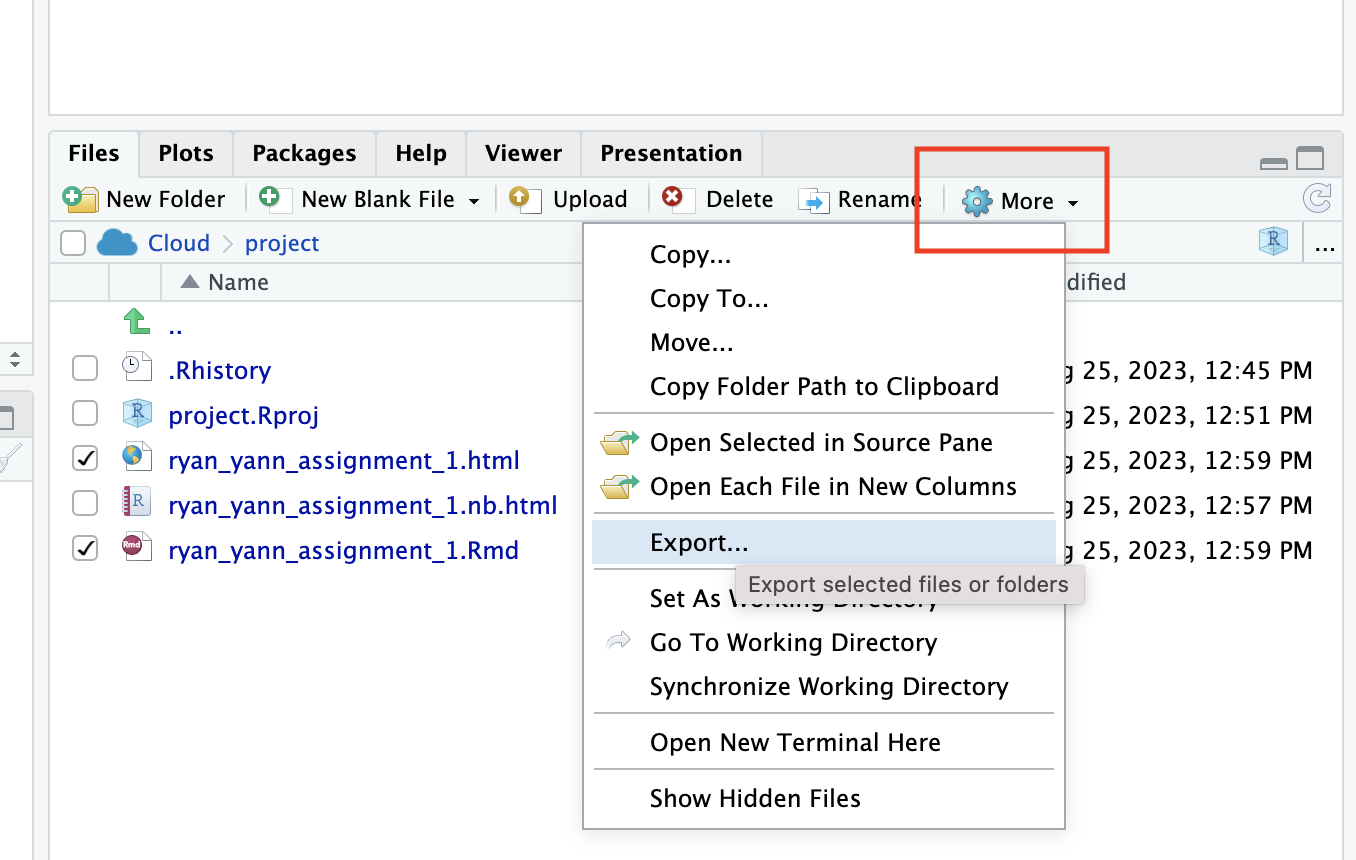
\includegraphics[width=6.25in,height=\textheight,keepaspectratio]{images/Screenshot 2023-08-25 at 13.02.31.png}

If you have correctly selected more than one file, Posit cloud will
automatically create a .zip file and download it. Save it with a
sensible name, and then you can upload this zip directly to Brightspace.

\textbf{This is the format we will use for every assignment, so it's
worth getting the hang of it!}

\subsection{Upload to Brightspace}\label{upload-to-brightspace}

Upload the .zip file to Brightspace in the assignment area.

\section{Adding Code}\label{adding-code}

To add a code block, use the menu items.

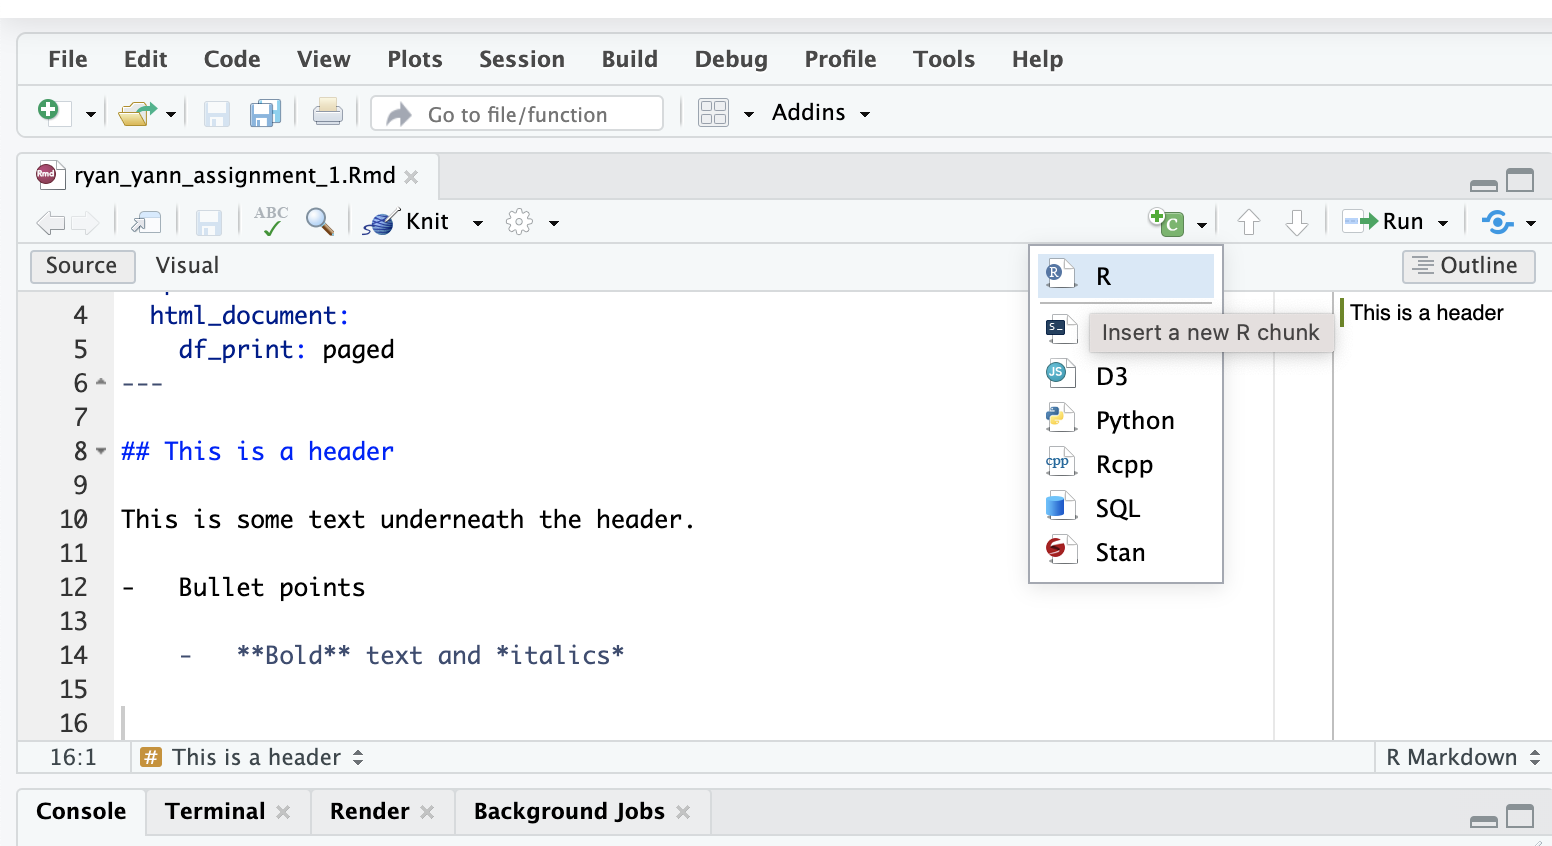
\includegraphics[width=6.25in,height=\textheight,keepaspectratio]{images/Screenshot 2023-08-25 at 13.05.07.png}

This will add a shaded area to your markdown file, called a `code cell'.

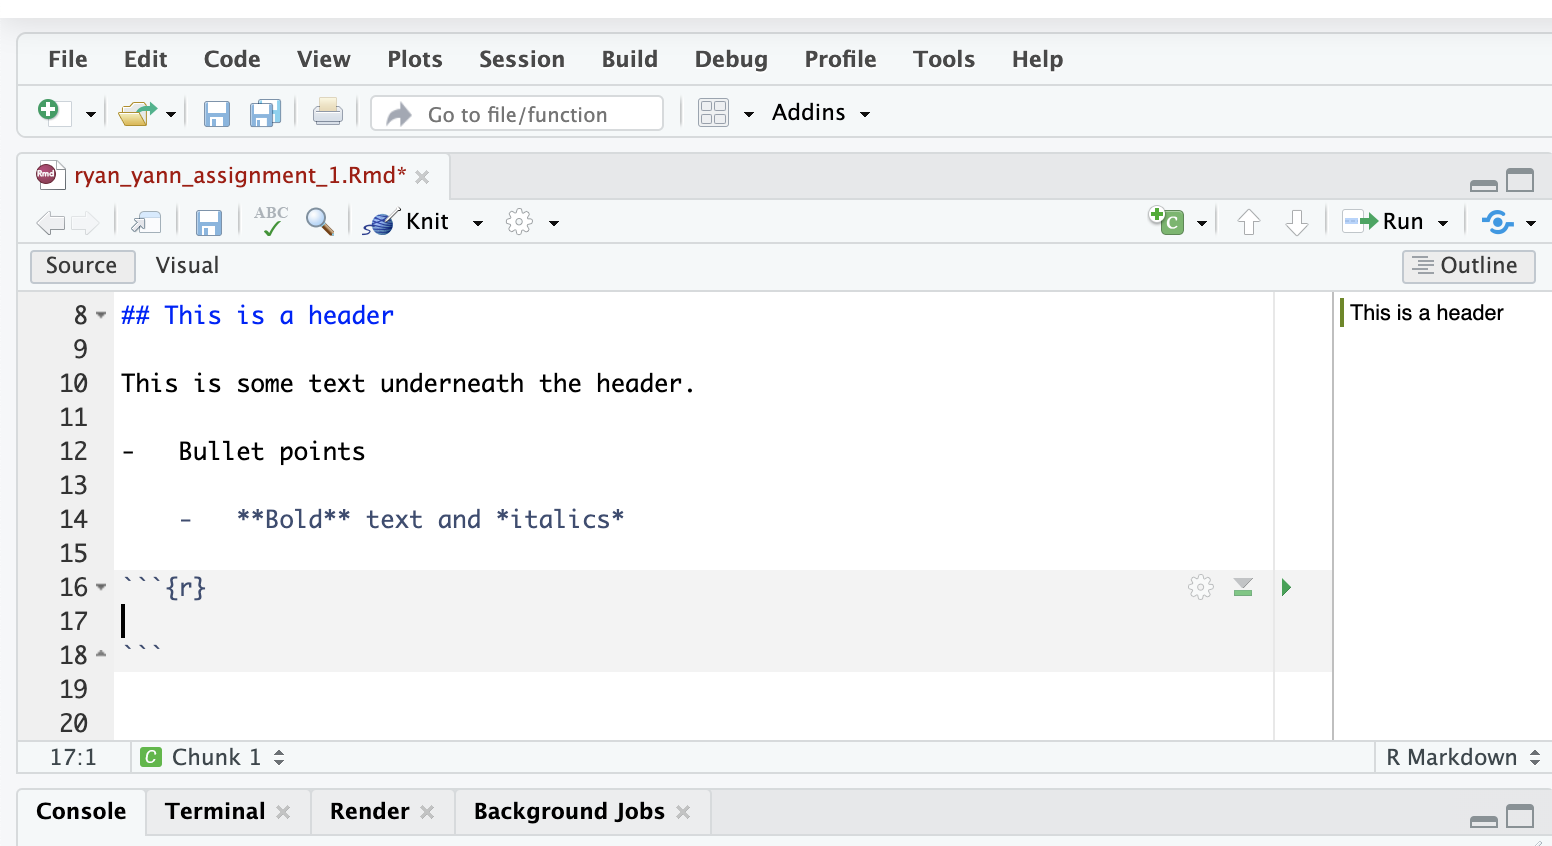
\includegraphics[width=6.25in,height=\textheight,keepaspectratio]{images/Screenshot 2023-08-25 at 13.05.31.png}

Add the simple code, 1 + 1. This will simply tell R to add these two
numbers together.

First, execute the code from the cell, without knitting the document.
Click on the green triangle in the top-right of the code cell. You'll
see that the output (2) appears below the cell.

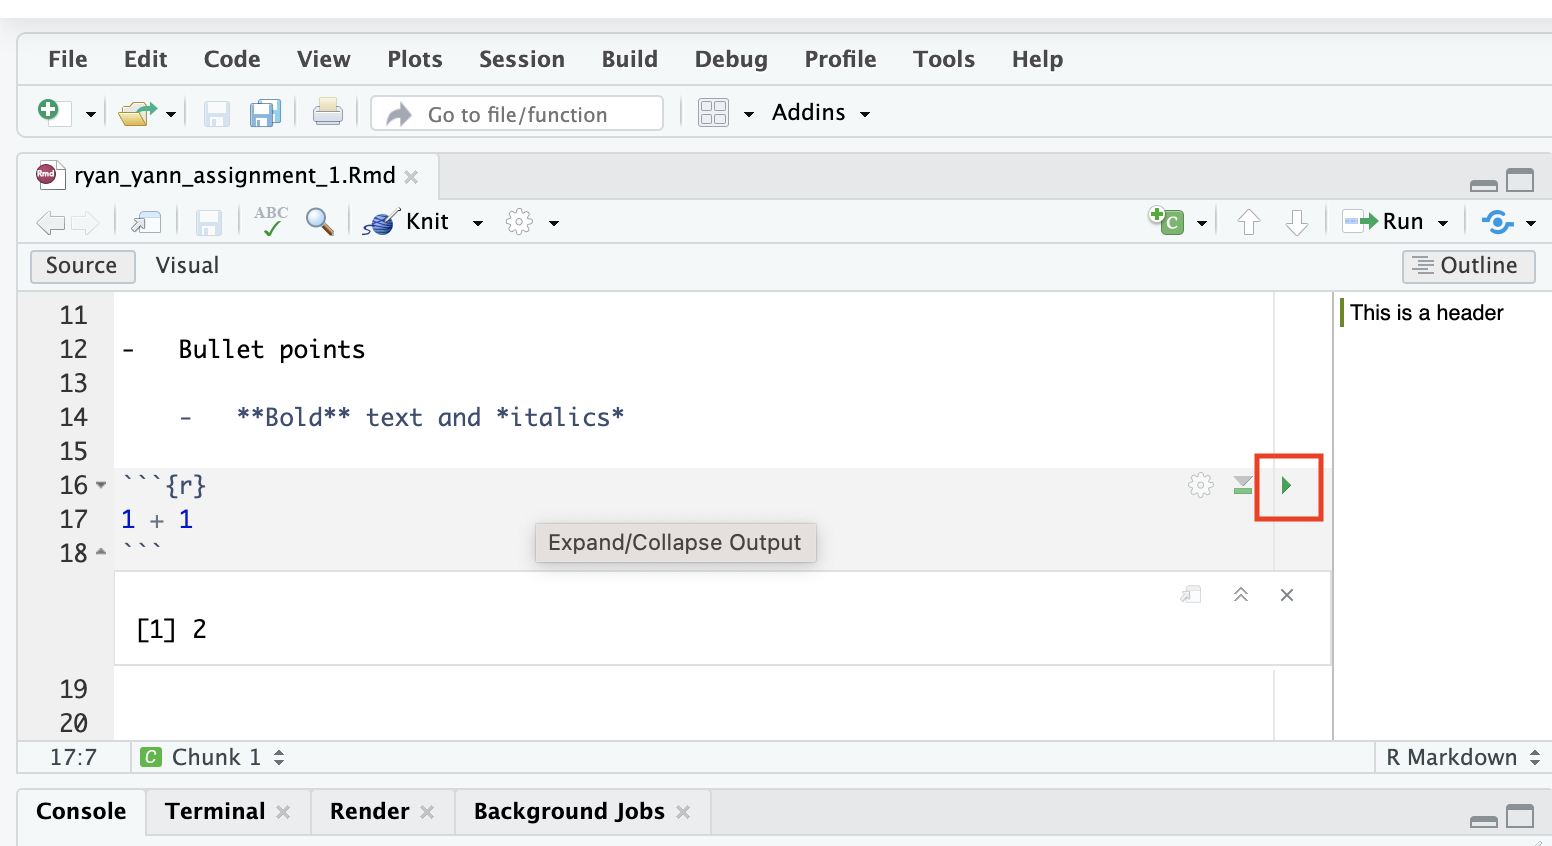
\includegraphics[width=6.25in,height=\textheight,keepaspectratio]{images/Screenshot 2023-08-25 at 13.07.20.png}

This is the code output. This output can be anything that we make in
code, such as a visualisation. This is what makes R markdown such a
great tool creating data visualisation reports. We can easily write up
text and findings, and publish them alongside code results, tables,
visualisations, even interactive maps.

Next, render/knit the document as in the last step. The document will
knit again. Look at the html file, and you'll see that the code is
displayed, and the code result - the output - is displayed underneath.

\section{Adding files}\label{adding-files}

The last thing we'll do is practise adding files to the Rstudio area.
Most times, you'll need to upload files to your workspace in order to
work with them. First, you'll up load them to the workspace, and second,
you'll read them into R.

You could also upload other files, for example if your final project
markdown includes some images not generated by code.

We'll practice this by downloading a file from Brightspace, and
uploading it to Posit Cloud. This file can be found under the `Files'
area on the course site. Download the file `box\_office' to your local
machine first.

To upload a file to Posit cloud, look at the file manager in the
bottom-right pane. Click on `Upload', and then browse to the file on
your computer, and click OK. You'll see the file appear in the file
browser in a moment.

\pandocbounded{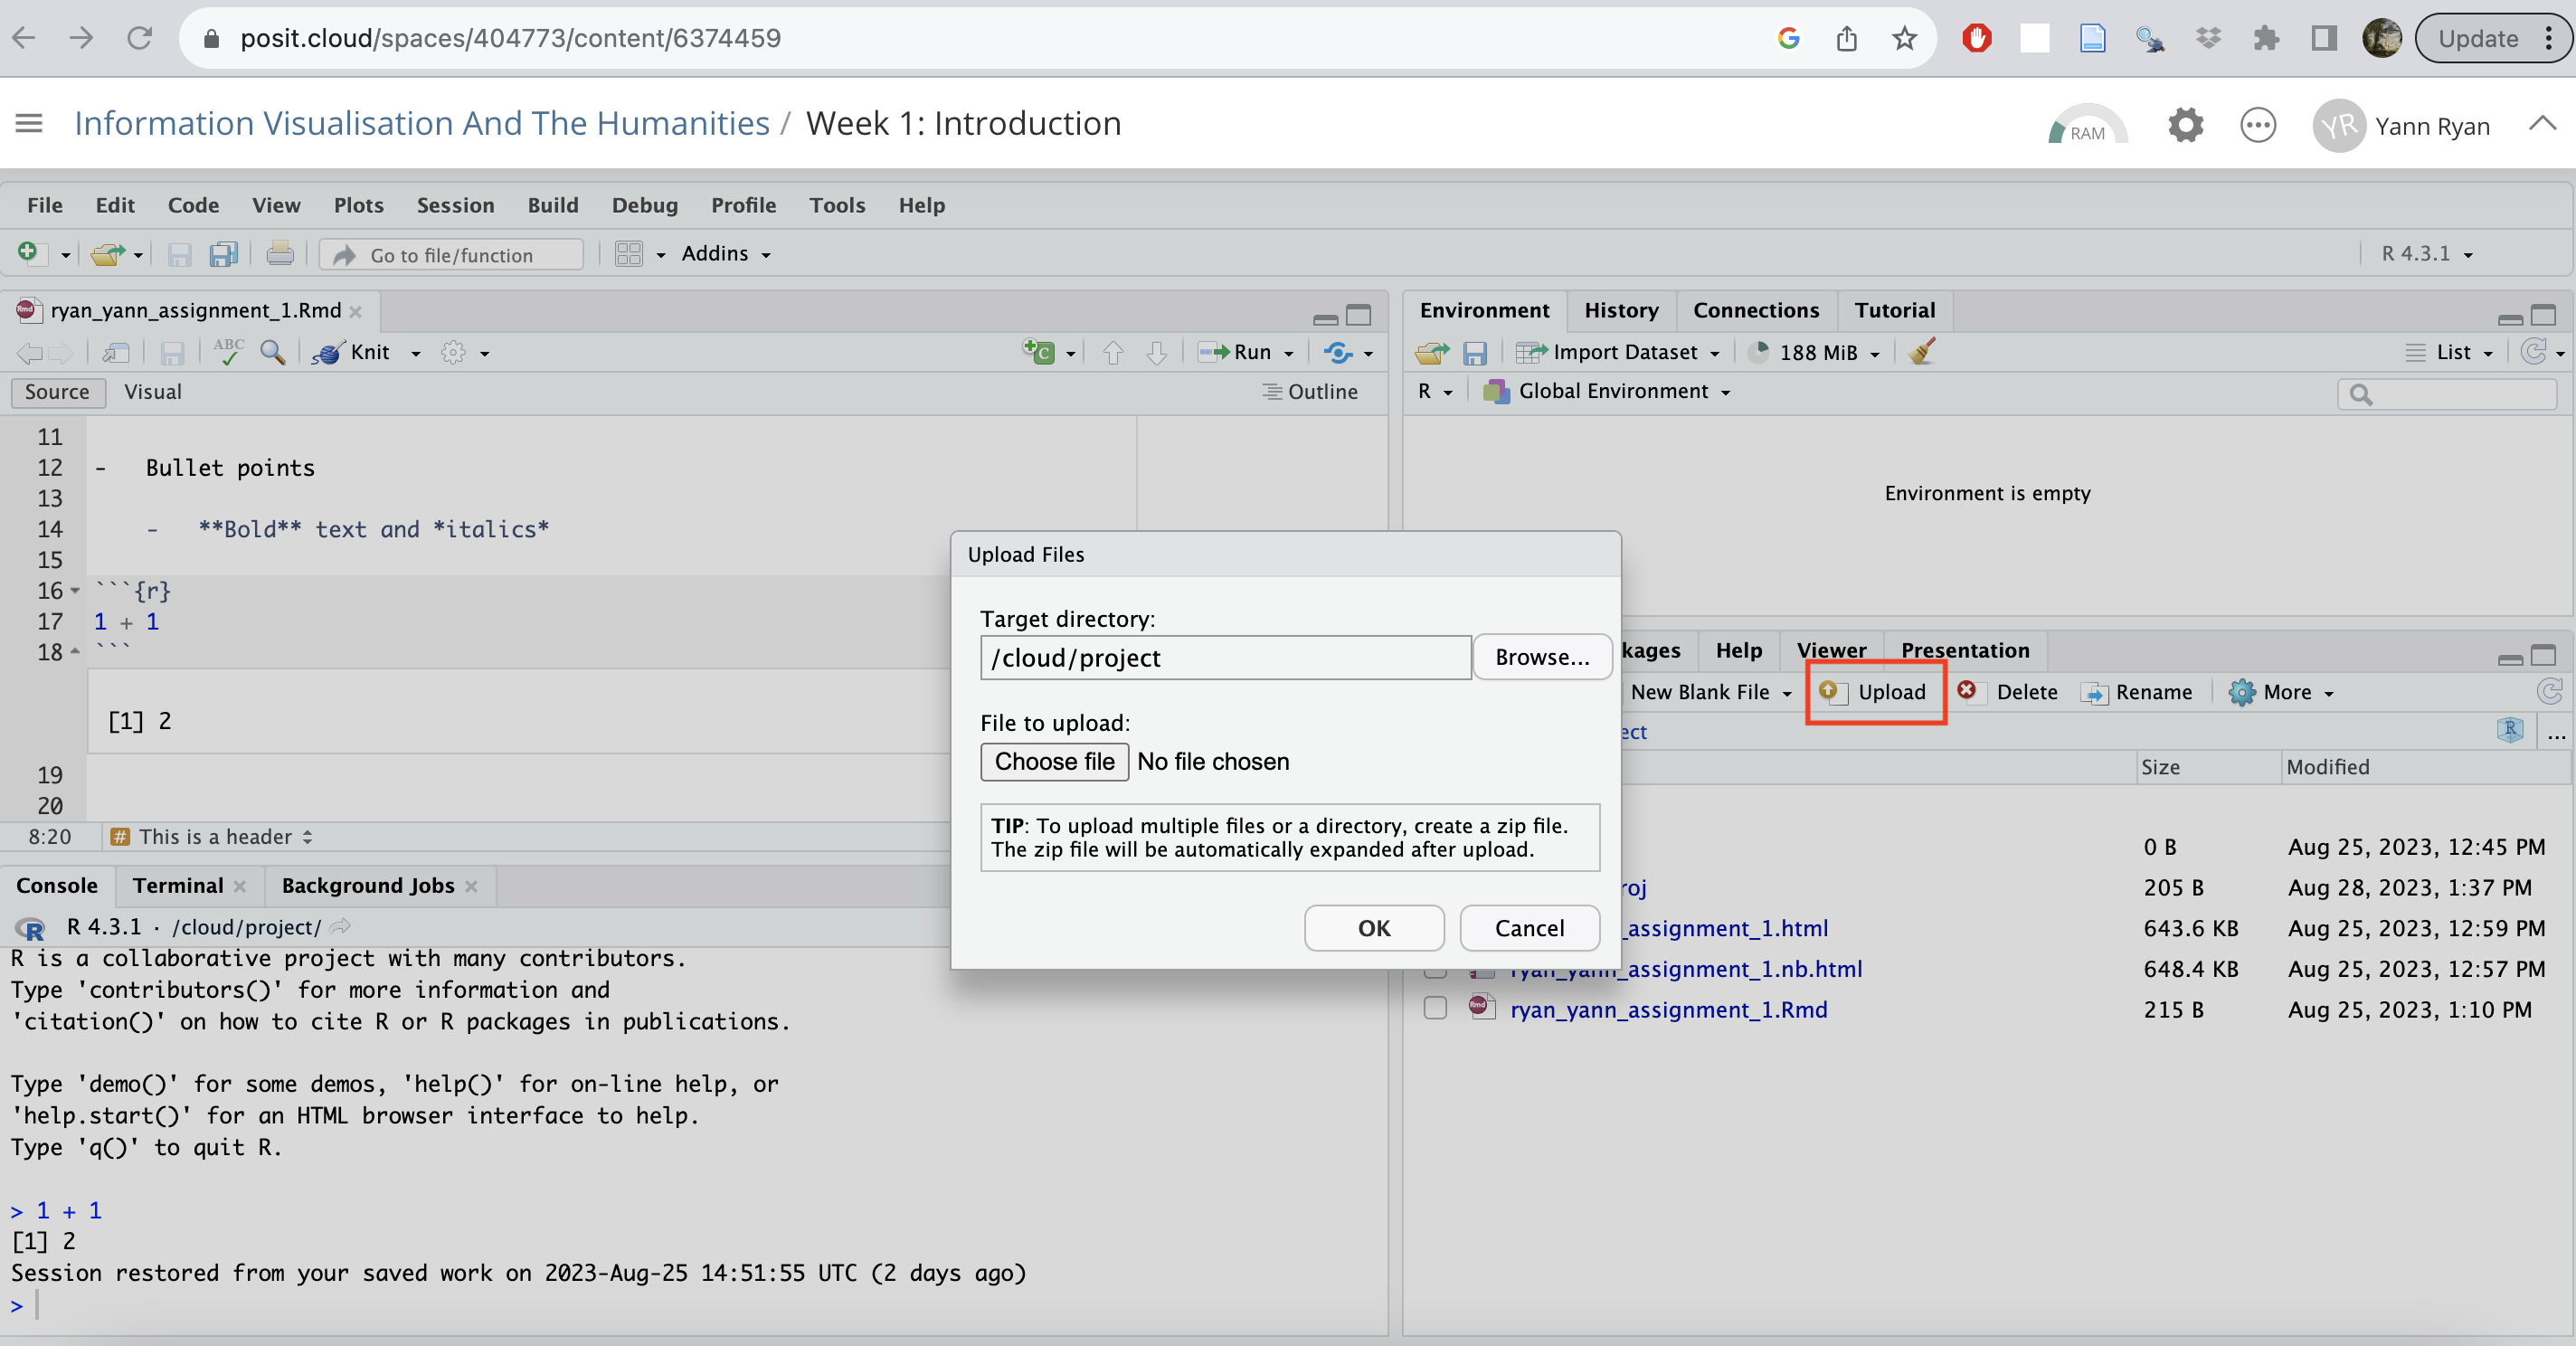
\includegraphics[keepaspectratio]{images/Screenshot 2023-08-28 at 13.39.27.png}}

\section{Environment}\label{environment}

Every time we create an object like this, it will appear within
RStudio's environment. This means it has been saved in memory as an
object which can be used for other purposes. When we close RStudio, the
environment disappears.

You can see the objects in the environment in the top-right corner (the
screenshot below will only show in the book version):

\pandocbounded{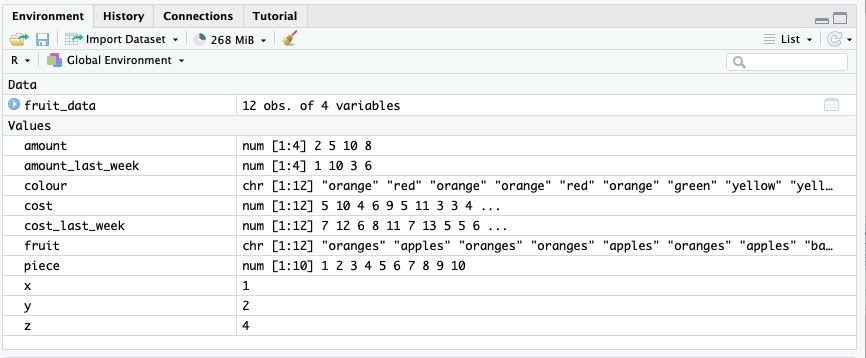
\includegraphics[keepaspectratio]{images/Screenshot 2023-09-05 at 15.26.02.png}}

Here you'll see everything we've created, and a preview of what it
contains. It's divided into \texttt{Data} and \texttt{Values}. Values
are the simple things we have created. We can see that x, for example,
is a single number: 4. \texttt{amount} is a vector of numbers.

Data contains any dataframes we have created. We can see we have created
one, called \texttt{fruit\_data}. We can also click on the
\texttt{fruit\_data} object to open it:

\pandocbounded{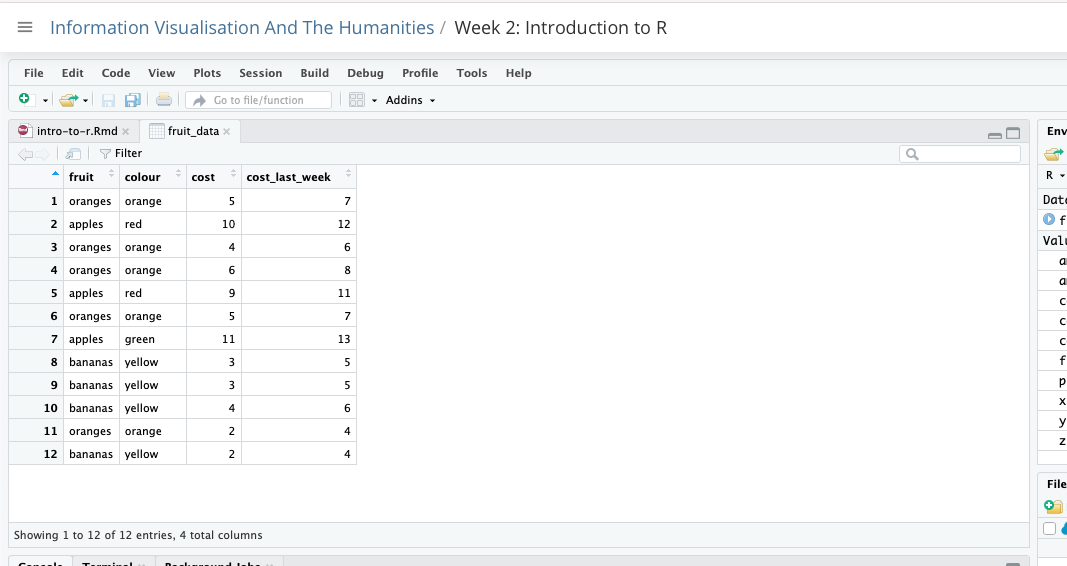
\includegraphics[keepaspectratio]{images/Screenshot 2023-09-05 at 15.26.17.png}}

Clicking on it will open a view of the dataframe in the top-left pane.
You'll see it looks much like a spreadsheet with rows and columns. This
can be very useful to see how your data looks and how it has been
imported.

You can close this tab or switch back to the .Rmd file to continue.

\section{Reading in external data}\label{reading-in-external-data}

Most of the time, you'll be working with external data sources. These
most commonly come in the form of comma separated values (.csv) or tab
separated values (.tsv). The tidyverse commands to read these are
\texttt{read\_csv()} and \texttt{read\_tsv}. You can also use
\texttt{read\_delim()}, and specify the type of delimited using
\texttt{delim\ =\ \textquotesingle{},\textquotesingle{}} or
\texttt{delim\ =\ \textquotesingle{}/t}. The path to the file is given
as a string to the argument \texttt{file=}.

\begin{Shaded}
\begin{Highlighting}[]
\NormalTok{df }\OtherTok{=} \FunctionTok{read\_csv}\NormalTok{(}\AttributeTok{file =} \StringTok{\textquotesingle{}top\_movie.csv\textquotesingle{}}\NormalTok{) }\CommentTok{\# Read a .csv file as a network, specify the path to the file here.}

\NormalTok{df}
\end{Highlighting}
\end{Shaded}

Notice that each column has a data type beside it, either for text or
for numbers. This is important if you want to sort or run calculations
on the data.

Advanced: \texttt{str\_¥}

\section{Learning Objectives}\label{learning-objectives-3}

Before moving on, take a look and see if you are confident with all of
the following learning objectives.

(the checkboxes are just for your own use, they won't save if you leave
or refresh the page)

\begin{itemize}
\item[$\square$]
  Open a Posit account and create a new notebook
\item[$\square$]
  Understand what an IDE is and how to code in it
\item[$\square$]
  Know how to create a code cell and how to write plain text in your
  notebook
\item[$\square$]
  Write some basic markdown
\item[$\square$]
  Export (knit) a file and download it to your local machine.
\end{itemize}

\section{}\label{section-1}

\chapter{Home exercises}\label{home-exercises}

\section{Instructions}\label{instructions}

The at-home exercises should be completed using Posit cloud. Log in to
your Posit account and open the project \texttt{Exercise\ 1}. Create a
new .Rmd file (use File -\textgreater{} New File -\textgreater{} R
Notebook.

I advise saving the new file straight away. Because you'll submit this
file as an assignment, use a standardised name:
exercise\_1\_lastname\_firstname. Regularly re-save the file.

When you have finished the exercise (or part of it), `knit' the file.
Export the .Rmd and the html as a .zip file, and upload this to the
assignment area.

\subsection{Exercise 1: work with variables and mathematical
operations}\label{exercise-1-work-with-variables-and-mathematical-operations}

\begin{figure}[H]

{\centering 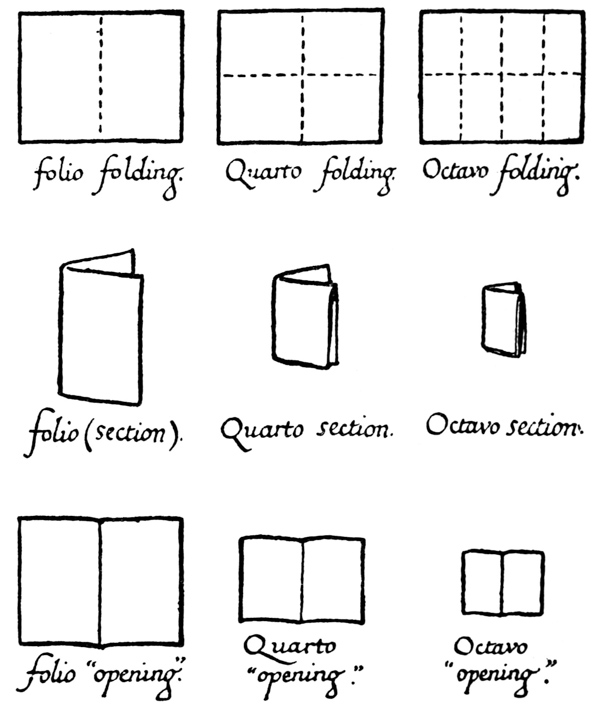
\includegraphics[width=2.1875in,height=\textheight,keepaspectratio]{images/book_sizes.jpg}

}

\caption{Illustration of book sizes. Found
\href{https://www.heathermollauthor.com/post/austen-and-folios-quartos-and-octavos}{here}}

\end{figure}%

You're working on a book history project, and you're interested in
finding out more about the most-used book formats. When books were still
made by hand (up until the beginning of the nineteenth century), books
were made by printing on a standard sized sheet of paper and then
folding the paper a number of times to make the pages. This process
determined the different sizes, or formats, of books.

The largest size (a single fold) was called \emph{folio}, followed by
\emph{quarto}, \emph{octavo}, and \emph{duodecimo}. (you might have
heard of the
\href{https://www.folger.edu/explore/shakespeare-in-print/first-folio/}{Shakespeare
`first folio'}, which is so named because it was the first time
Shakespeare was published in folio format - individual plays had
previously been
\href{https://www.folger.edu/explore/shakespeare-in-print/diy-quarto/}{published
as quarto}).

\begin{tcolorbox}[enhanced jigsaw, coltitle=black, bottomrule=.15mm, title=\textcolor{quarto-callout-note-color}{\faInfo}\hspace{0.5em}{Why does this matter?}, leftrule=.75mm, colframe=quarto-callout-note-color-frame, breakable, toprule=.15mm, opacityback=0, bottomtitle=1mm, toptitle=1mm, colback=white, rightrule=.15mm, titlerule=0mm, left=2mm, arc=.35mm, opacitybacktitle=0.6, colbacktitle=quarto-callout-note-color!10!white]

In the study of the book (bibliography), determing the format is
important: folio-sized books were reserved for important and expensive
publications which were meant to last. In a real-world example, we could
do this on a large dataset of information from a book catalogue, to look
for patterns and changes over time. In that case, we would usually do a
similar calculation, but over a whole column of numbers.

\end{tcolorbox}

\subsubsection{Steps}\label{steps}

\begin{enumerate}
\def\labelenumi{\arabic{enumi}.}
\item
  In a first code cell, create two variables, called
  \texttt{book\_height} and \texttt{book\_width}. Set each to a number:
  make up some realistic values for book height and width in milimetres.
\item
  In a new code cell, write code that will multiply them together, and
  save this as a variable \texttt{book\_area}.
\item
  Now, let's calculate the area of a typical folio book. A full sheet of
  paper measured 500 x 740 mm. In a new code cell, write code to
  calculate the area, in millimeters squared, of a folio page
  (\textbf{remember the full sheet of paper is also folded in half to
  make the page}).
\end{enumerate}

Any book which has an area equal or larger than this is considered folio
size.

\begin{enumerate}
\def\labelenumi{\arabic{enumi}.}
\setcounter{enumi}{3}
\tightlist
\item
  In a new code cell, write code to do this comparison using the
  variables created above.
\end{enumerate}

See below for the answer if you get stuck:

\begin{Shaded}
\begin{Highlighting}[]
\NormalTok{book\_height }\OtherTok{\textless{}{-}} \DecValTok{500}

\NormalTok{book\_width }\OtherTok{\textless{}{-}} \DecValTok{700}

\NormalTok{book\_area }\OtherTok{\textless{}{-}}\NormalTok{ book\_height }\SpecialCharTok{*}\NormalTok{ book\_width}

\NormalTok{folio\_area }\OtherTok{\textless{}{-}}\NormalTok{ (}\DecValTok{500} \SpecialCharTok{*} \DecValTok{740}\NormalTok{) }\SpecialCharTok{/} \DecValTok{2} \CommentTok{\# the width multiplied by the height, divided by two}

\NormalTok{book\_area }\SpecialCharTok{\textgreater{}=}\NormalTok{ folio\_area }\CommentTok{\# check if book area is greater than or equal to folio\_area.}
\end{Highlighting}
\end{Shaded}

\begin{verbatim}
[1] TRUE
\end{verbatim}

\subsection{Exercise two: create and compare two
vectors}\label{exercise-two-create-and-compare-two-vectors}

\begin{enumerate}
\def\labelenumi{\arabic{enumi}.}
\tightlist
\item
  Create a vector containing the names of Beyoncé's top-selling albums:
  \emph{I am Sasha Fierce}, \emph{Dangerously in Love}, \emph{B'Day},
  \emph{Beyoncé}, and \emph{4}.
\end{enumerate}

\begin{tcolorbox}[enhanced jigsaw, coltitle=black, bottomrule=.15mm, title=\textcolor{quarto-callout-tip-color}{\faLightbulb}\hspace{0.5em}{Tip}, leftrule=.75mm, colframe=quarto-callout-tip-color-frame, breakable, toprule=.15mm, opacityback=0, bottomtitle=1mm, toptitle=1mm, colback=white, rightrule=.15mm, titlerule=0mm, left=2mm, arc=.35mm, opacitybacktitle=0.6, colbacktitle=quarto-callout-tip-color!10!white]

Usually when you create vectors, you can use either single or double
quotation marks. What happens when you try to use single quotation marks
here?

What happens to the fifth album title? Is it stored as a number or as
characters?

\end{tcolorbox}

\begin{enumerate}
\def\labelenumi{\arabic{enumi}.}
\setcounter{enumi}{1}
\item
  Write code in a new code cell which checks if any of the strings in
  the vector are equal to ``Renaissance''
\item
  Create a new vector, containing the titles of the top 5 ranked albums
  from this \emph{Variety} article: \emph{Renaissance}, \emph{Beyoncé},
  \emph{Lemonade}, \emph{4}, and \emph{B'Day}.
\item
  Now, check if any of these top-ranked albums are missing from the
  top-selling list.
\end{enumerate}

\begin{tcolorbox}[enhanced jigsaw, coltitle=black, bottomrule=.15mm, title=\textcolor{quarto-callout-tip-color}{\faLightbulb}\hspace{0.5em}{Tip}, leftrule=.75mm, colframe=quarto-callout-tip-color-frame, breakable, toprule=.15mm, opacityback=0, bottomtitle=1mm, toptitle=1mm, colback=white, rightrule=.15mm, titlerule=0mm, left=2mm, arc=.35mm, opacitybacktitle=0.6, colbacktitle=quarto-callout-tip-color!10!white]

The easiest way to compare two vectors is to use another command,
\texttt{\%in\%}. This essentially says, check each of the elements of
this vector to see if they are equal to any of the elements of this
second vector:

e.g., \texttt{vector\_1\ \%in\%\ vector\_2}

\end{tcolorbox}

\subsubsection{}\label{section-2}




\end{document}
